\chapter{Towards an ellipsoidal characterization of in vivo upper-limb force feasible sets}
\label{chapter:5}

\usection{Introduction}
\emph{In vivo} isometric force feasible sets represent all possible isometric forces exertable at a point of application in a given posture. Assuming these sets are convex, their surface is defined by the maximal exertable forces. This thesis focuses specifically on such forces at the hand of the right upper limb: it allows to define the biomechanical force limits of an individual in order to improve a robot assistance within a physical Human-Robot interaction. 

Characterizing these sets \emph{in vivo} involves gathering multiple maximal voluntary contractions (MVICs) in a specific posture, as detailed in Chapter \ref{chapter:1}. However, generalizing from a limited number of force measurements to a complete set representation presents a challenge. One approach is to collect enough measurements to describe these sets as \emph{polytopes}. Yet, this characterization, when considering \emph{in silico} force polytopes by means of a musculoskeletal model, requires the assumption that muscles can produce maximal joint torques independently, neglecting muscle tension dependencies. Chapter \ref{chapter:2} also emphasized the computationally complex process required to force polytope manipulation.

Alternative representations may be more suitable. Chapter \ref{chapter:3} suggested that with a sufficiently large number of muscles, force feasible sets resemble ellipsoids, regardless of specific muscle activation patterns - as long as they are assumed to produce a convex muscle tension set. Muscle tension relations then only affects the ellipsoid's scaling. While this \emph{large} number ideally approaches infinity for a perfect ellipsoidal approximation, Chapter \ref{chapter:4} provides numerical evidence that 50 muscles in a musculoskeletal model yield similar variability patterns for both polytopic and ellipsoidal representations. Thus, we consider 50 muscles sufficient for applying an ellipsoidal representation, assuming equivalence between the two.

Building on these theoretical foundations, this chapter focuses on the \emph{in vivo} ellipsoidal characterization of force feasible sets using the general isometric formulation of \emph{in silico} force feasible sets established in Chapter \ref{chapter:1}. We collect MVICs in four upper-limb postures from ten participants and evaluate the extent to which these measurements support an ellipsoidal representation. Since Chapter \ref{chapter:4} hinted that the muscle geometry may not be the most influencial type of parameters in a personalized musculoskeletal model derived from a generic one, we assume that only a scaled musculoskeletal model and personalized force-generating parameters are required to represent \emph{in vivo} force feasible sets. Consequently, this chapter seeks to validate this assumption. We shall thus first measure multiple maximal isometric force of an individual in various postures and then compute \emph{in silico} force ellipsoids with personalized force-generating parameters in a scaled musculoskeletal model. Then, if the personalized \emph{in silico} force ellipsoids closely approximate the minimal volume ellipsoid encompassing the measured forces (which captures the geometric properties - size, orientation, translation - of the measured forces in a unique manner), it indicates that \emph{in silico} force ellipsoids are a valid representation of \emph{in vivo} force feasible sets.

A successful validation would indicate that while measured force feasible sets may not be perfectly ellipsoidal, their behavior (orientation, elongation) can be effectively described by ellipsoids constructed from a projection-then-intersection force feasible set paradigm. This simplification reduces computational complexity for set-based optimization and, importantly, reduces the experimental burden to nine MVICs, as nine points sufficiently define an ellipsoid. Besides, Chapter \ref{chapter:4} also indicated that the muscle geometry may not be of strong interest when personalizing a musculoskeletal model to predict \emph{in vivo} force feasible sets, which was already hinted in Chapter \ref{chapter:4} - but only \emph{in silico}.

Section \ref{sec:experimental_setup} details the experimental process for gathering MVICs, with an adaptable setup accommodating anthropometric variations and different postures. Section \ref{sec:posture_stability} assesses posture stability during these unconstrained exertions. Finally, Section \ref{sec:experimental_reconstruction} explores \emph{in vivo} force feasible set reconstruction from the measured forces and, by incorporating biomechanical assumptions about force production at the hand, evaluates the suitability of ellipsoidal \emph{in silico} force feasible set models (Chapter \ref{chapter:3}). The chapter concludes with a discussion on the validity of the ellipsoidal representation and the associated biomechanical assumptions for \emph{in silico} modeling.


\section{Design of an adaptable experimental platform for MVIC}
\label{sec:experimental_setup}
As recalled in Chapter \ref{chapter:1}, describing the force feasible set of an individual upper limb at the hand requires measuring maximal voluntary isometric contractions (MVIC) in multiple directions. We therefore employed an experimental protocol similar to those described in (\cite{rezzougUpperLimbIsometricForce2021b}) and (\cite{hernandezIsometricForceCapabilities2015}), where the individual is in a sitting position on a comfortable chair.

We designed a setup whose main goal was to adapt the MVIC protocol to the anthropometric variability of the participants. The following subsections describe its design.

\subsection{Isolation of forces exerted by upper-limb muscles}
During the experiment, a participant must exert MVIC using his right upper-limb muscles only. While challenging, as abdominal muscles and inherent back motion may be involved during such an exertion, the setup was designed to minimize the influence of other body parts. The participant was seated in a sturdy car seat sufficiently elevated from the ground to ensure his feet did not touch the ground. The seat was mounted on a wood stand made of 5 wooden pallets (144 mm height) using large screws.

Furthermore, when exerting maximal force with only the upper limb, participants naturally tend to engage their back muscles and abdominals, leading to back deformation. To reduce possible movements occurring in the back and the right shoulder, shoulder and abdomen strips were tightened over the participant and served to stabilize both the back and the shoulders, as shown in Figures \ref{fig:chair_elevated} and \ref{fig:chair_shoulder}.
\begin{figure}[!htb]
    \centering
    \begin{minipage}{0.49\linewidth}
        \captionsetup{justification=centering}
        \centering
        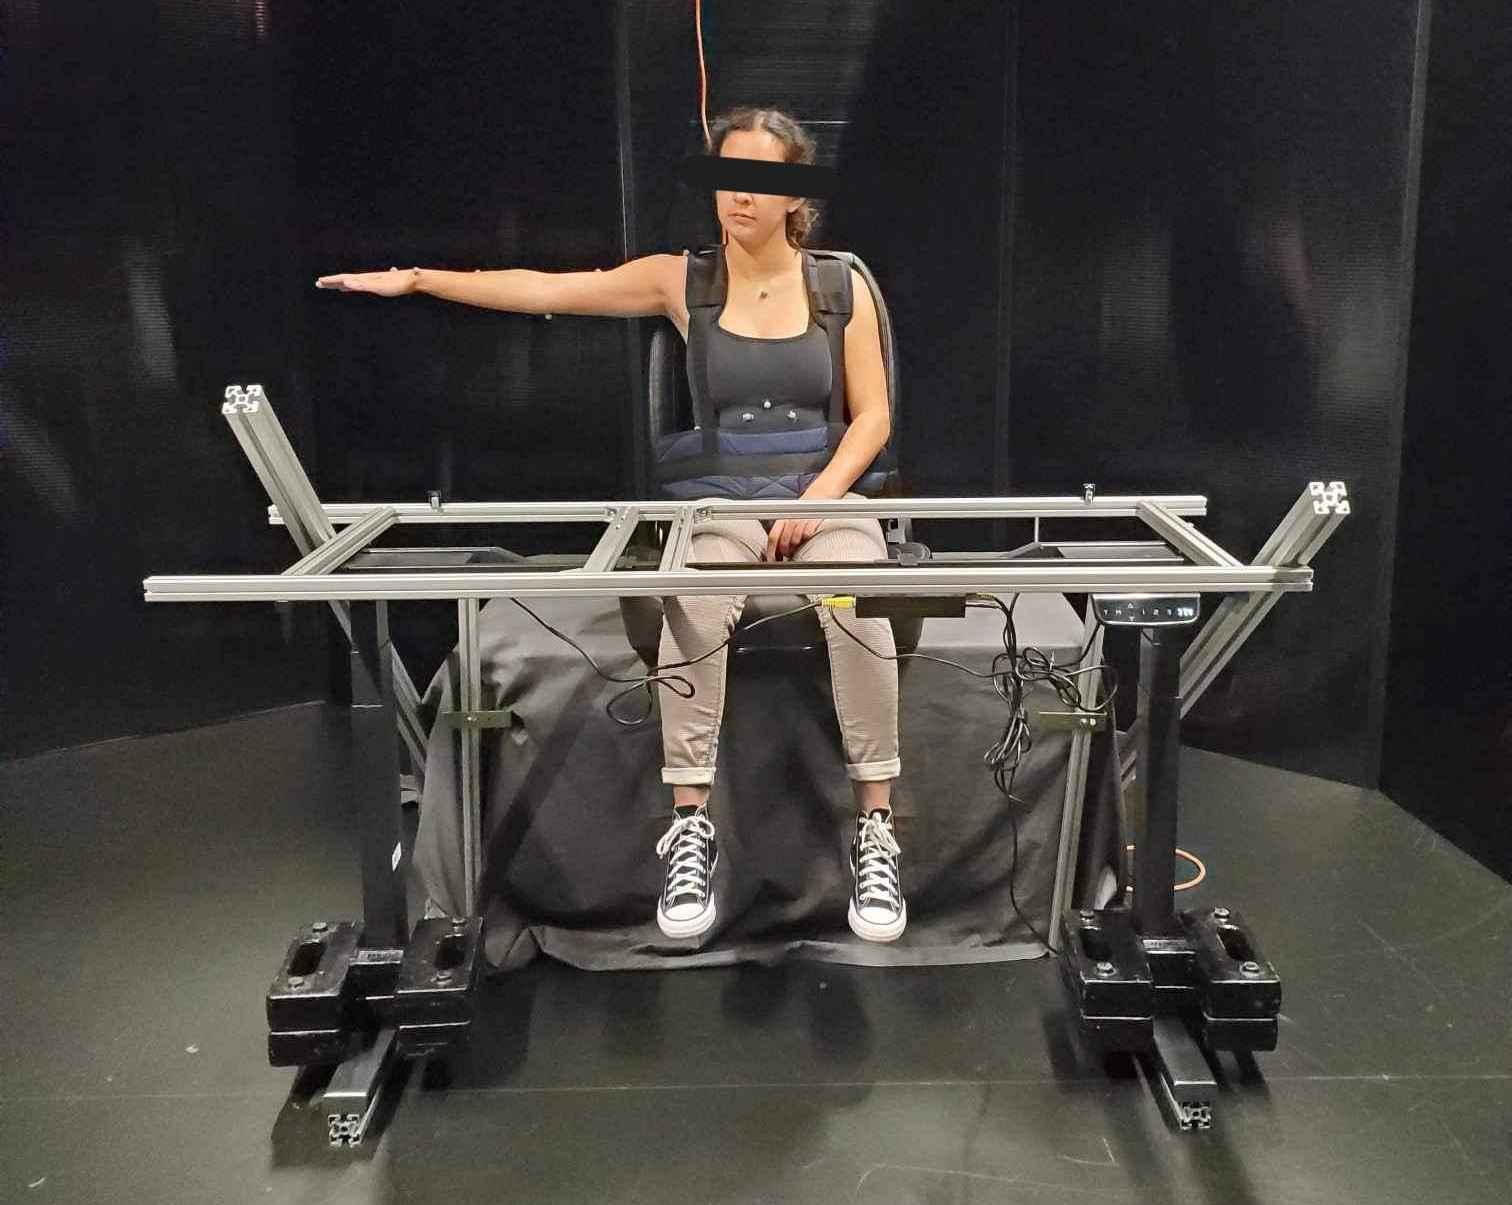
\includegraphics[clip, width=1\linewidth]{img/chapter_5/chair_elevated_01_cut.jpg}
        \caption{The participant feet do not touch the ground. The left arm was left loose in between the legs to avoid possible contact forces.}
        \label{fig:chair_elevated}
    \end{minipage}
    \hfill
    \begin{minipage}{0.49\linewidth}
        \captionsetup{justification=centering}
        \centering
        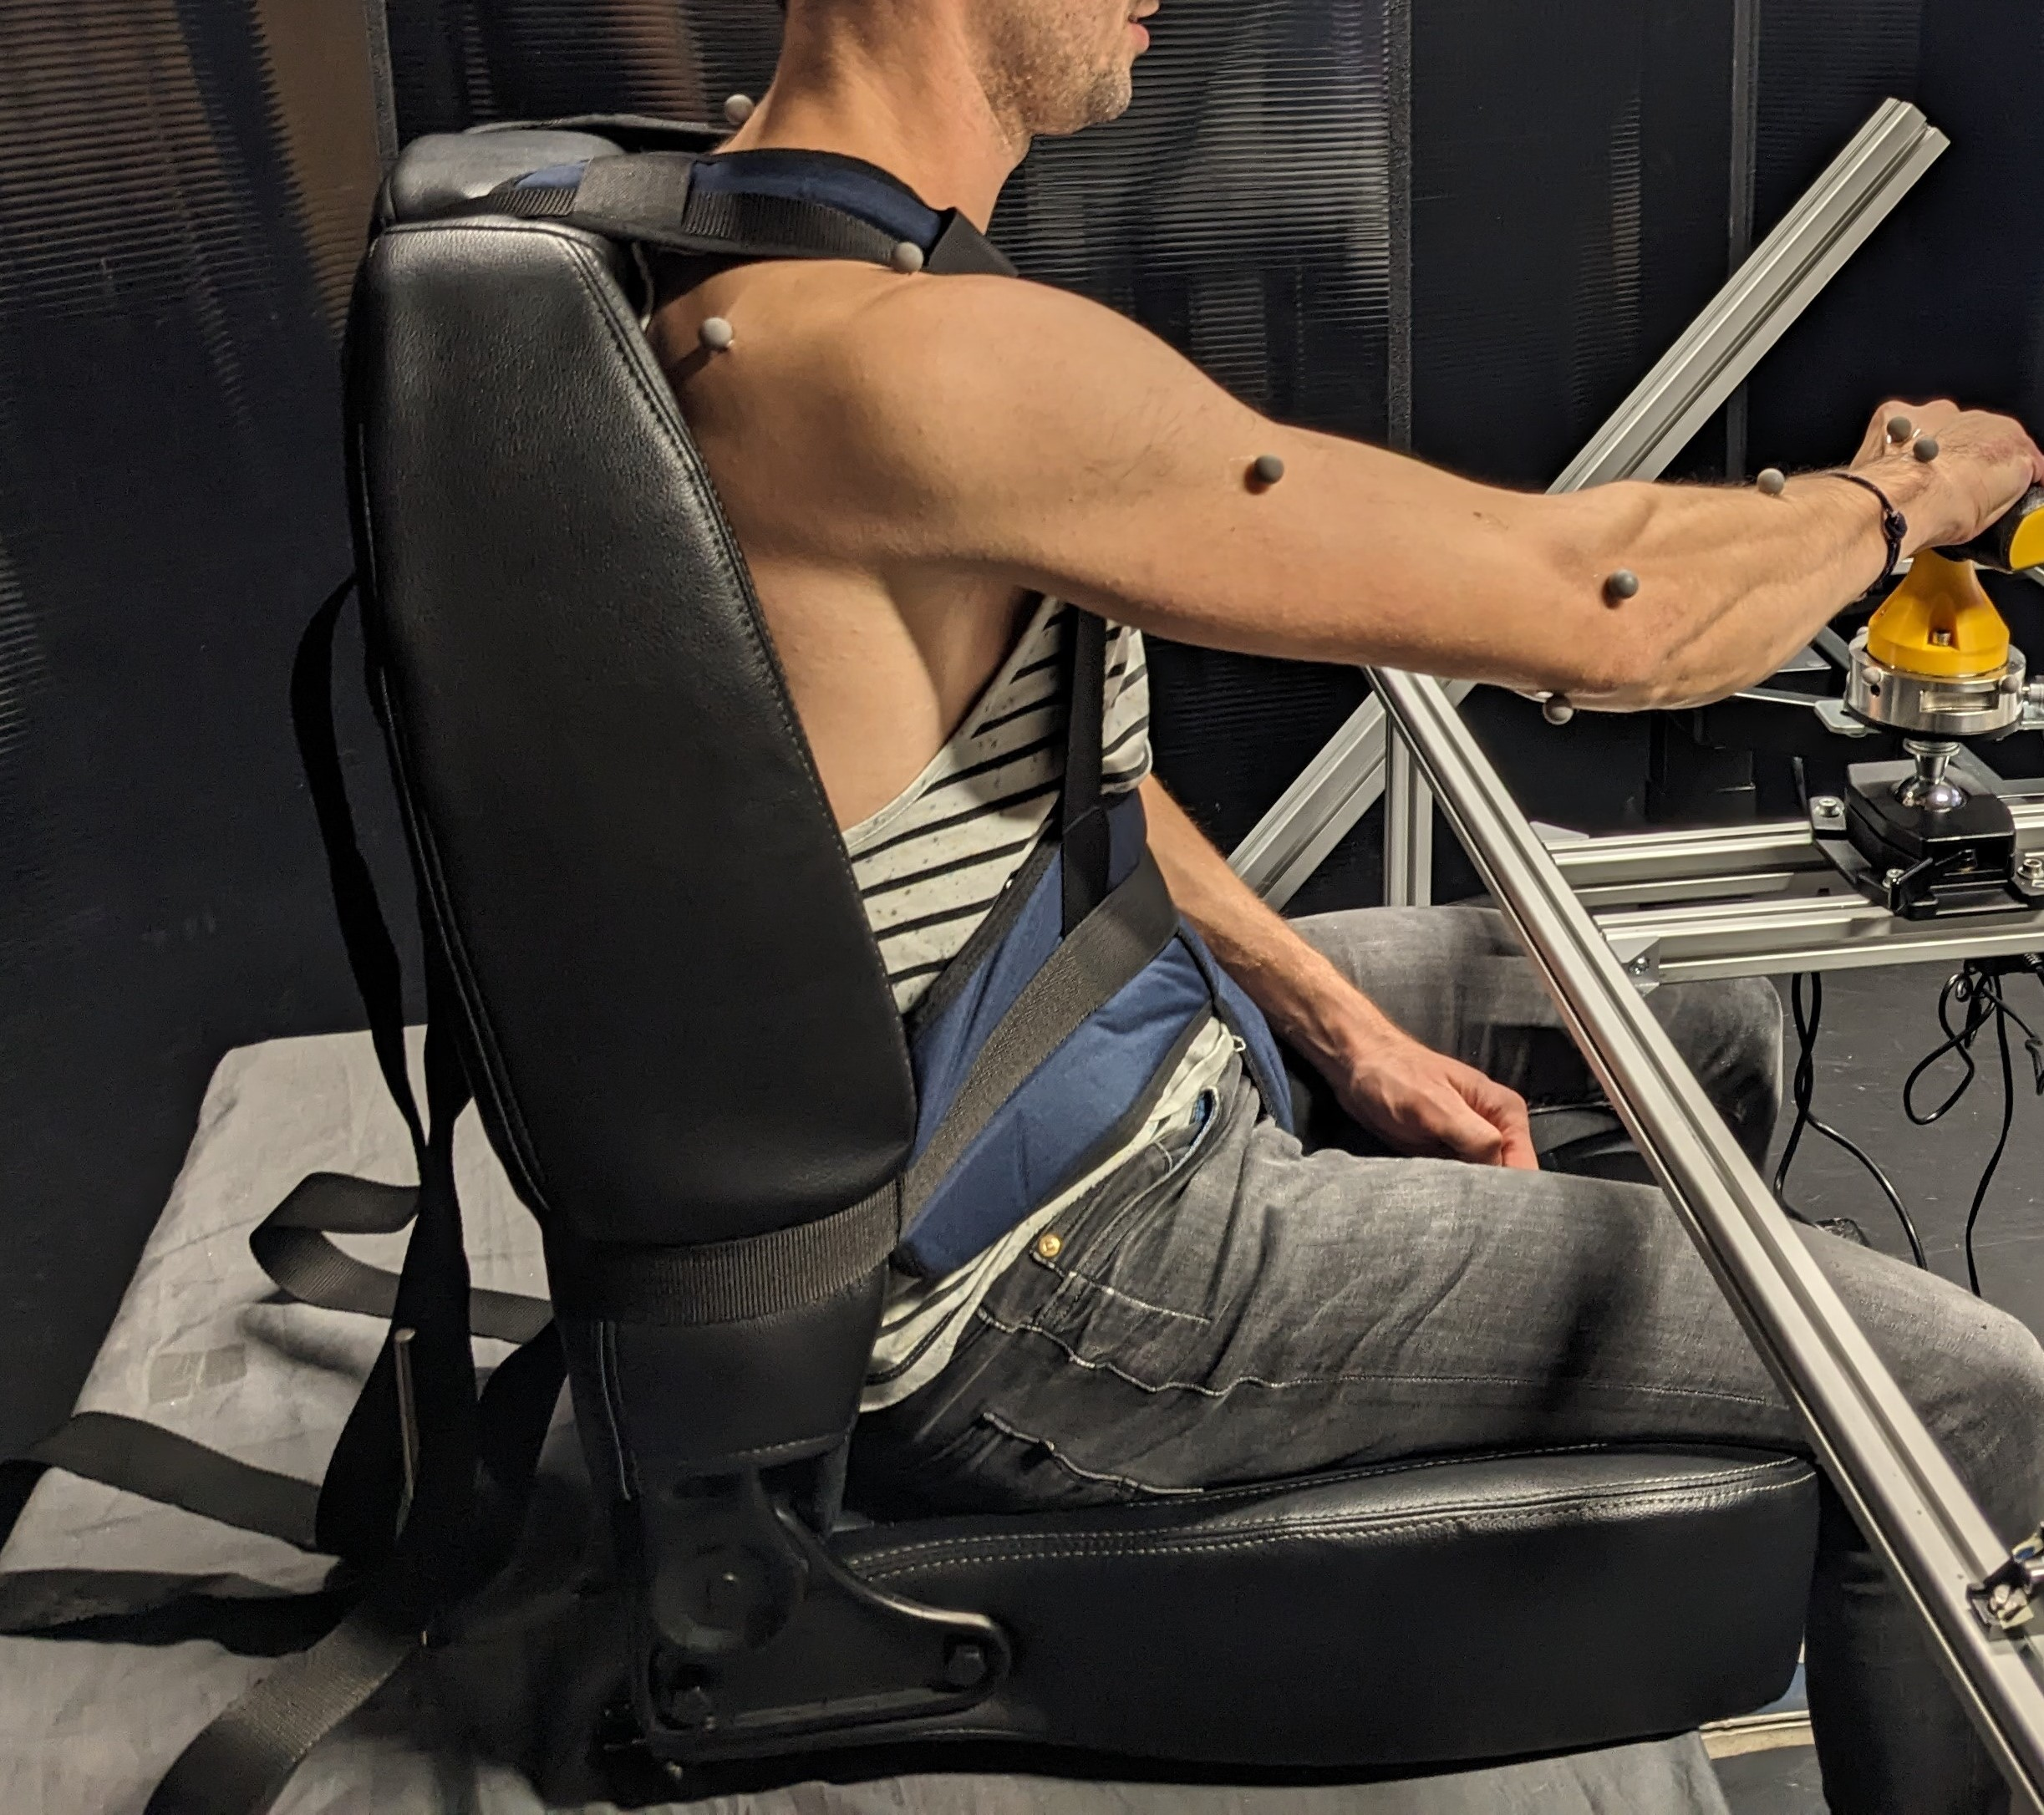
\includegraphics[clip, width=0.9\linewidth]{img/chapter_5/chair_stabilize_shoulder_.jpg}
        \caption{The shoulder and abdomen strips ensure a straight back. The shoulders translations are also strongly limited in range, in order to allow only rotations.}
        \label{fig:chair_shoulder}
    \end{minipage}
\end{figure}

\subsection{Anthropometric variability and hand location}

Adapting the setup also required addressing the challenge of positioning the force/torque sensor at the participant's hand for a given upper-limb posture. Based on previous MVIC protocols that involved grasping (\cite{crosbyHandStrengthNormative1994}; \cite{watanabeShortTermReliabilityGrip2005}), we designed a horizontal handle to be grasped by the hand and attached it to a 6-axes ATI Delta Force/Torque sensor with an acquisition frequency of 1000 Hz (Figure \ref{fig:ati_delta_force_torque}). Anti-slip strips were wrapped around the handle to prevent slippage due to sweat. To account for the rotational position of the hand, the sensor was mounted on a metal ball with restricted rotational movement (Figure \ref{fig:handle_force_torque}).

\begin{figure}[!htb]
    \begin{minipage}{0.49\linewidth}
        \captionsetup{justification=centering}
        \centering
        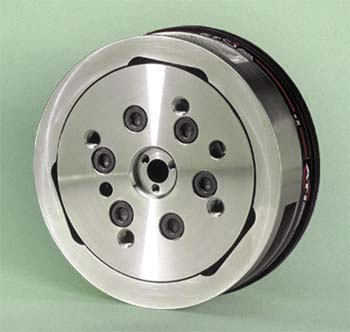
\includegraphics[clip, width=0.6\linewidth]{img/chapter_5/ati_delta_force_torque.jpg}
        \caption{ATI Delta 6-axes force/torque sensor.}
        \label{fig:ati_delta_force_torque}
    \end{minipage}
    \hfill
    \begin{minipage}{0.49\linewidth}
        \centering
        \captionsetup{justification=centering}
        \begin{minipage}{0.49\linewidth}
            \centering
            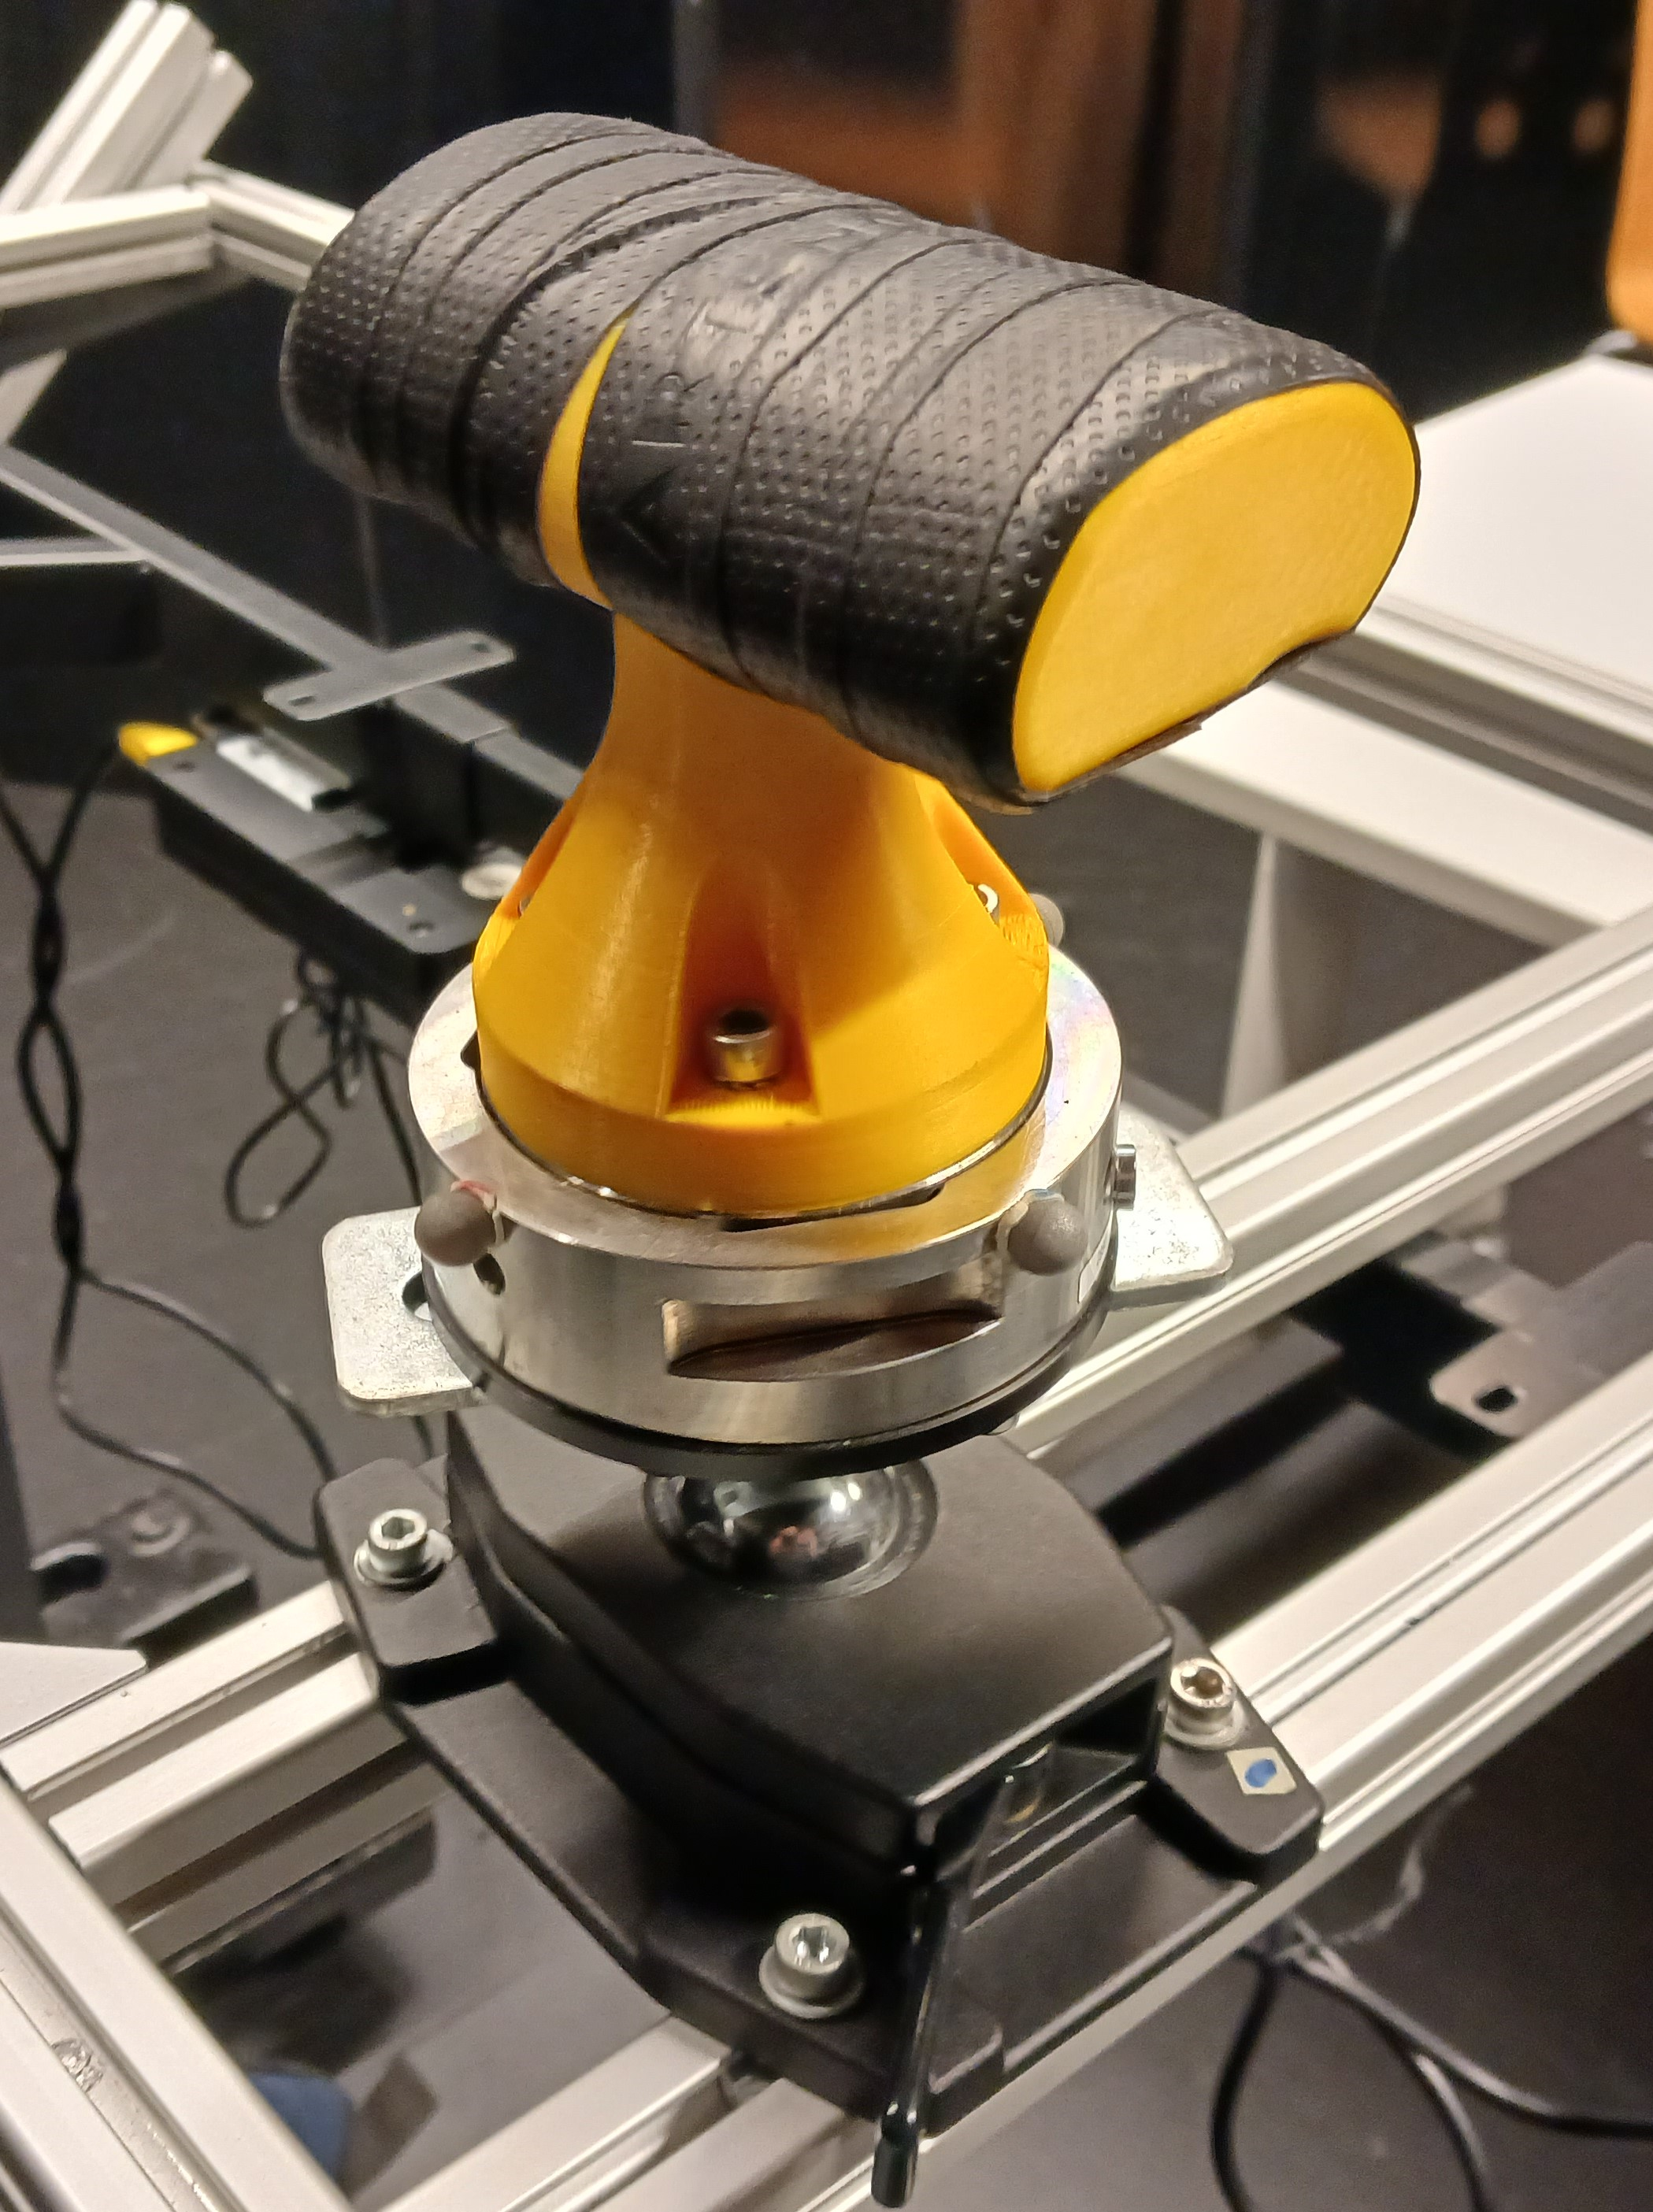
\includegraphics[clip, width=0.92\linewidth]{img/chapter_5/handle_01.jpg}
        \end{minipage}
        \hfill
        \begin{minipage}{0.49\linewidth}
            \centering
            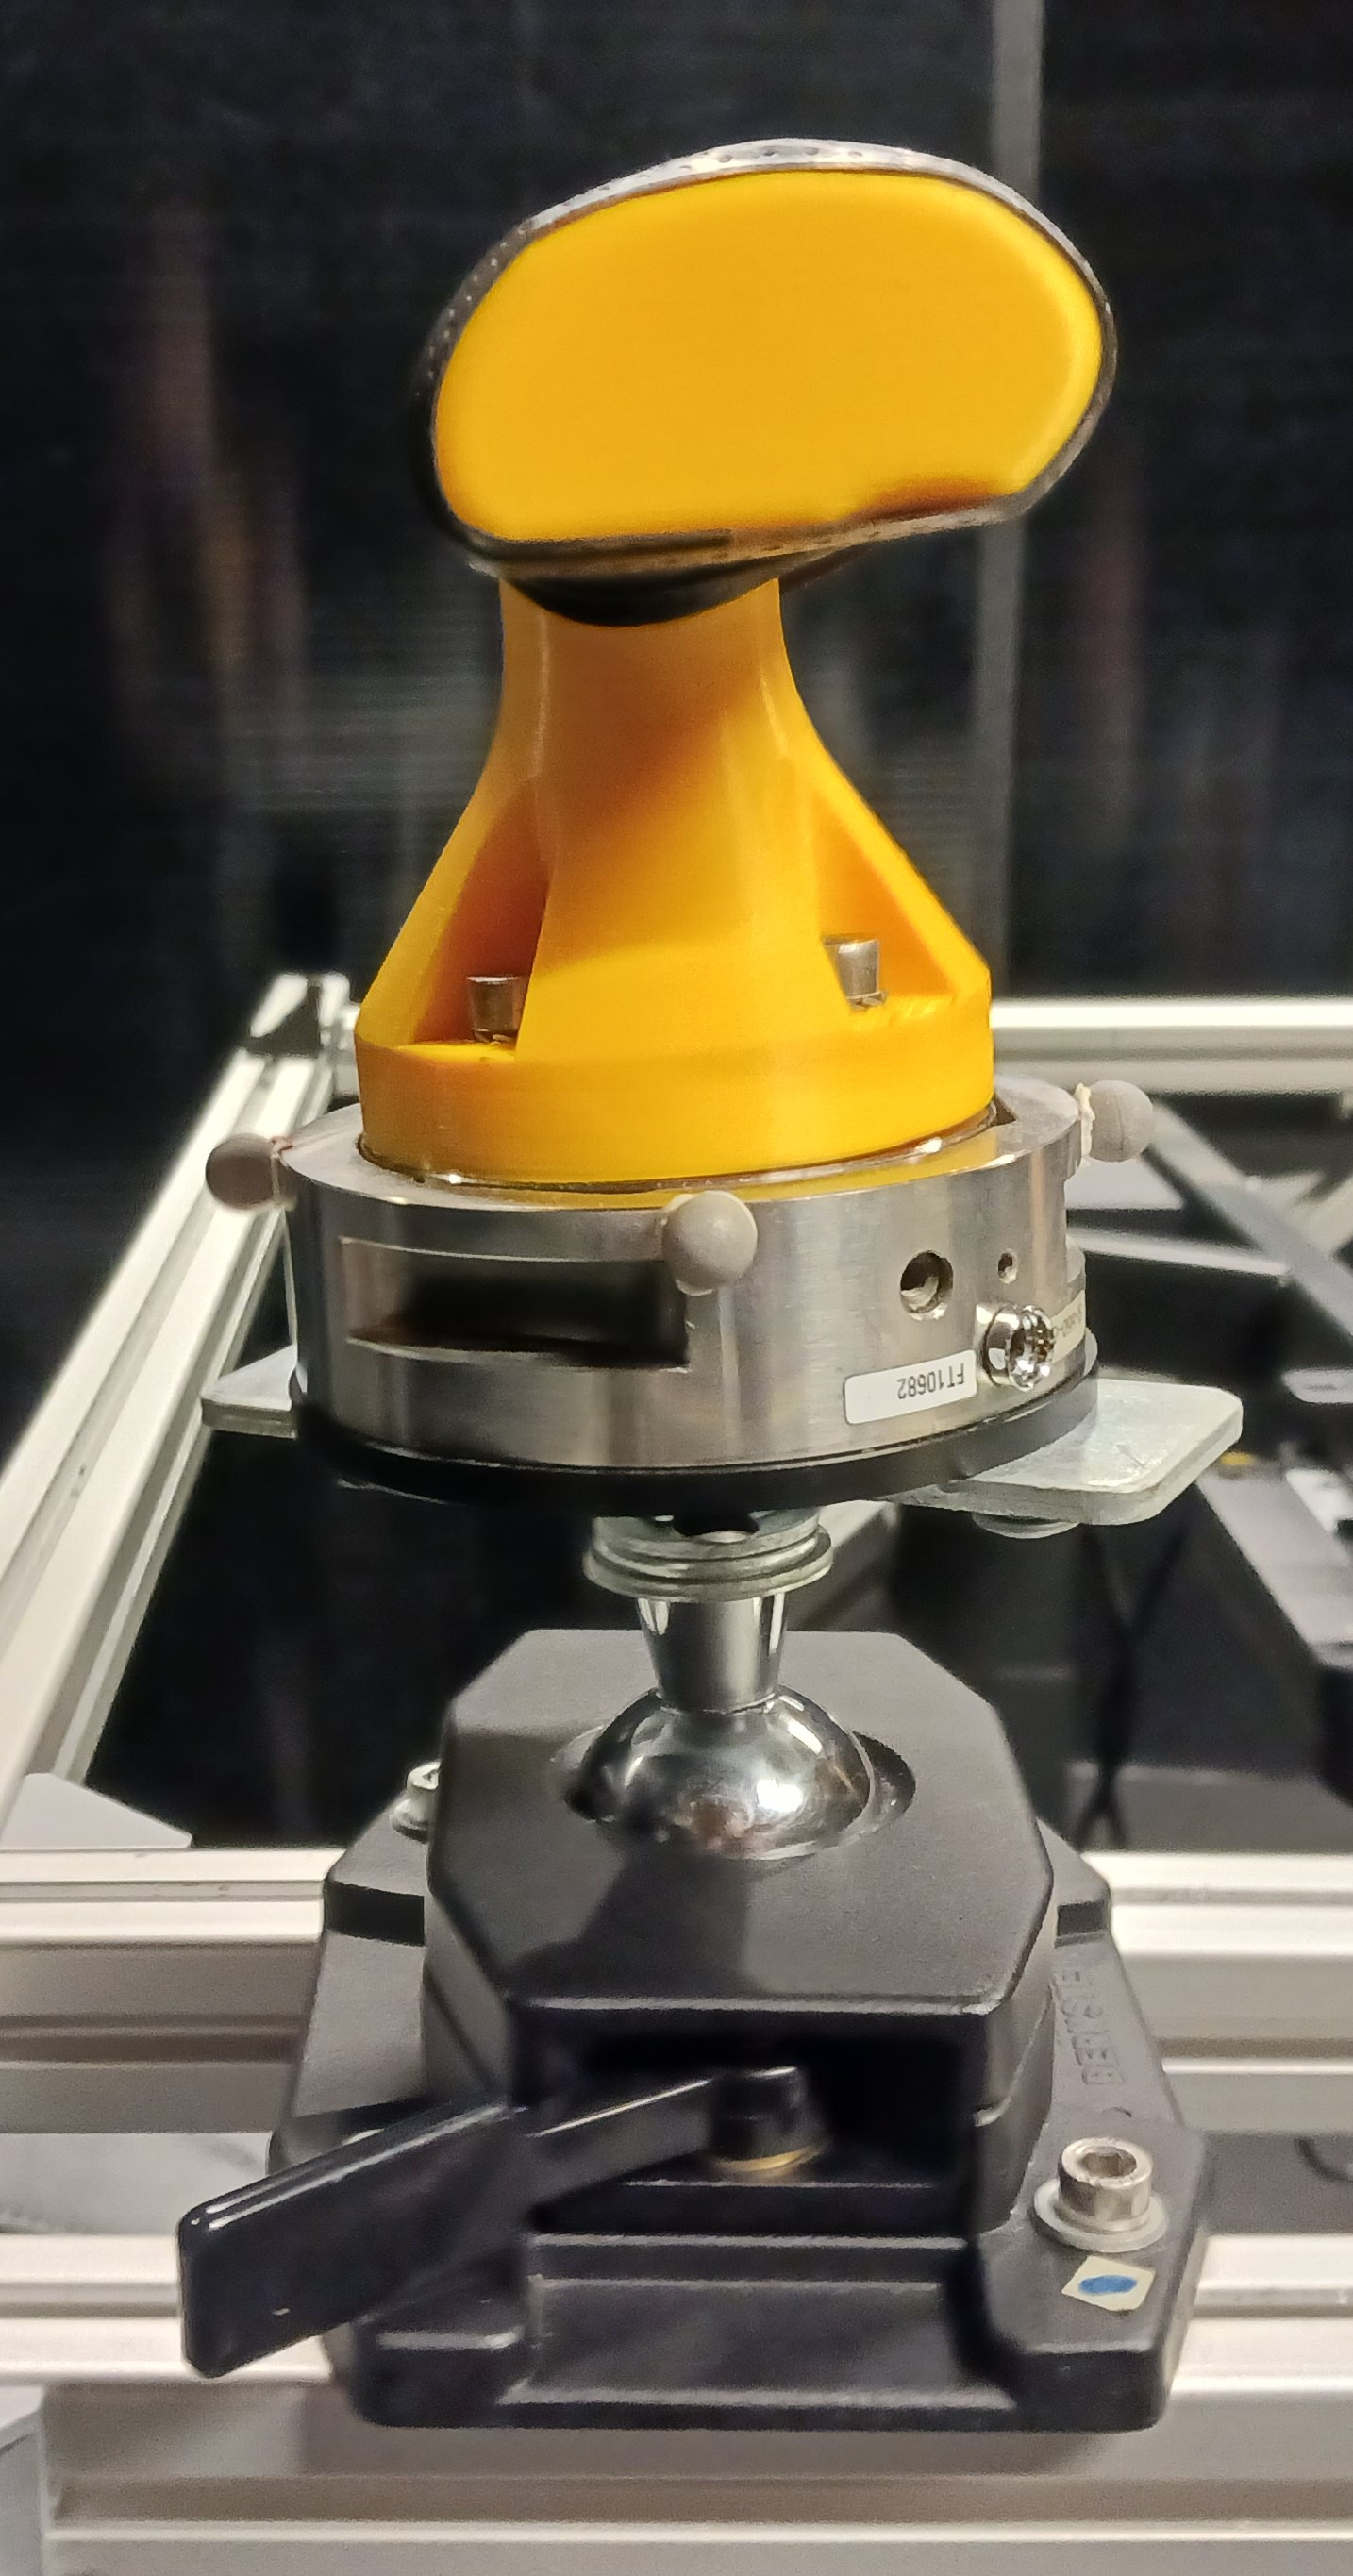
\includegraphics[clip,width=0.65\linewidth]{img/chapter_5/handle_02.jpg}
        \end{minipage}
        \caption{The handle fixed on top of the force/torque sensor ensures a comfortable and anti-slip grasp.}
        \label{fig:handle_force_torque}
    \end{minipage}

\end{figure}

To achieve accurate placement, the force/torque sensor needed to be adjustable along all three axes. A height-adjustable table with electric controls addressed vertical positioning. For depth and horizontal positioning, a custom-made aluminum profile support system was mounted on the table. To counteract potential deformation of the table at higher heights, two aluminum profiles were fixed to its sides and attached directly to the base of the wooden stand.

\begin{figure}[!htb]
    \captionsetup{justification=centering}
    \centering
    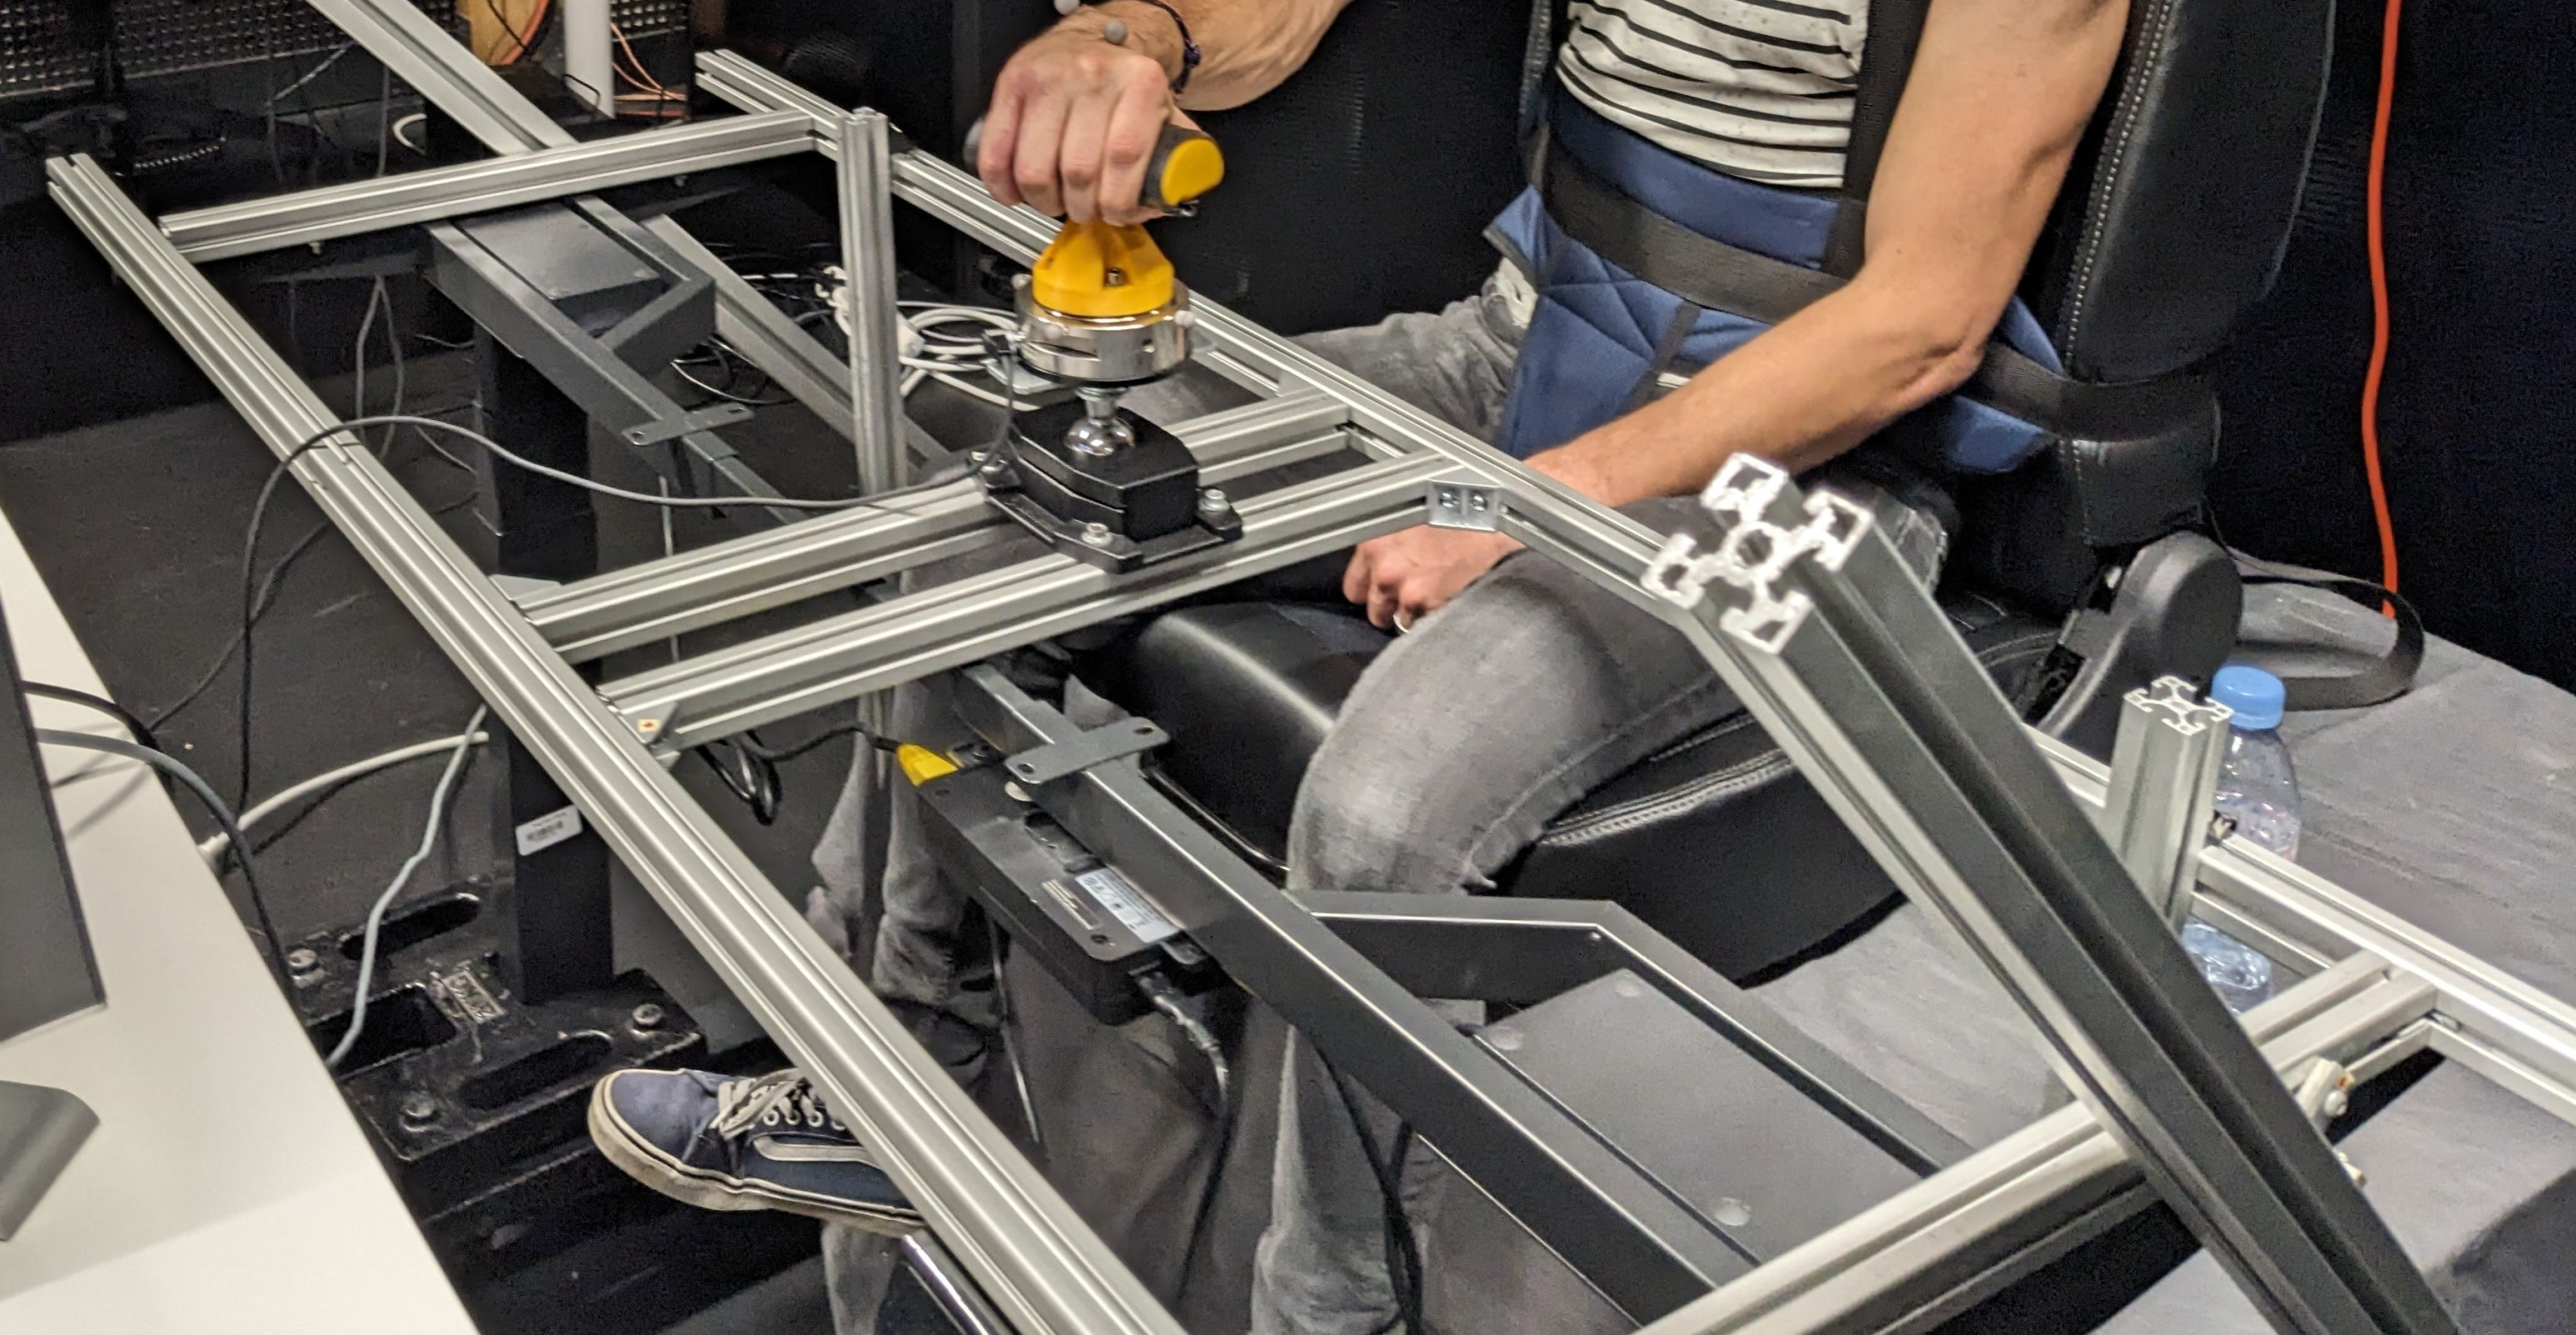
\includegraphics[clip, width=0.8\linewidth]{img/chapter_5/mounted_table.jpg}
    \caption{This adjustable custom-made aluminum profile support allows for precise positioning of the force/torque sensor to accommodate participants of different sizes and varying upper limb postures.}
    \label{fig:mounted_table}
\end{figure}

\subsection{Force directions and real-time visual force feedback}
In the Cartesian force space, 26 directions have been defined as combinations of azimuth angles (ranging from 0° to 315° relative to the horizontal forearm axis in 45° steps) and elevation angles (-45°, 0°, and 45° relative to the horizontal plane), and two additional vertical directions corresponding to 90° and -90° elevation (Fig. \ref{fig:rezzoug_hernandez_directions_}).

\begin{figure}[!htb]
    \captionsetup{justification=centering}
        \centering
        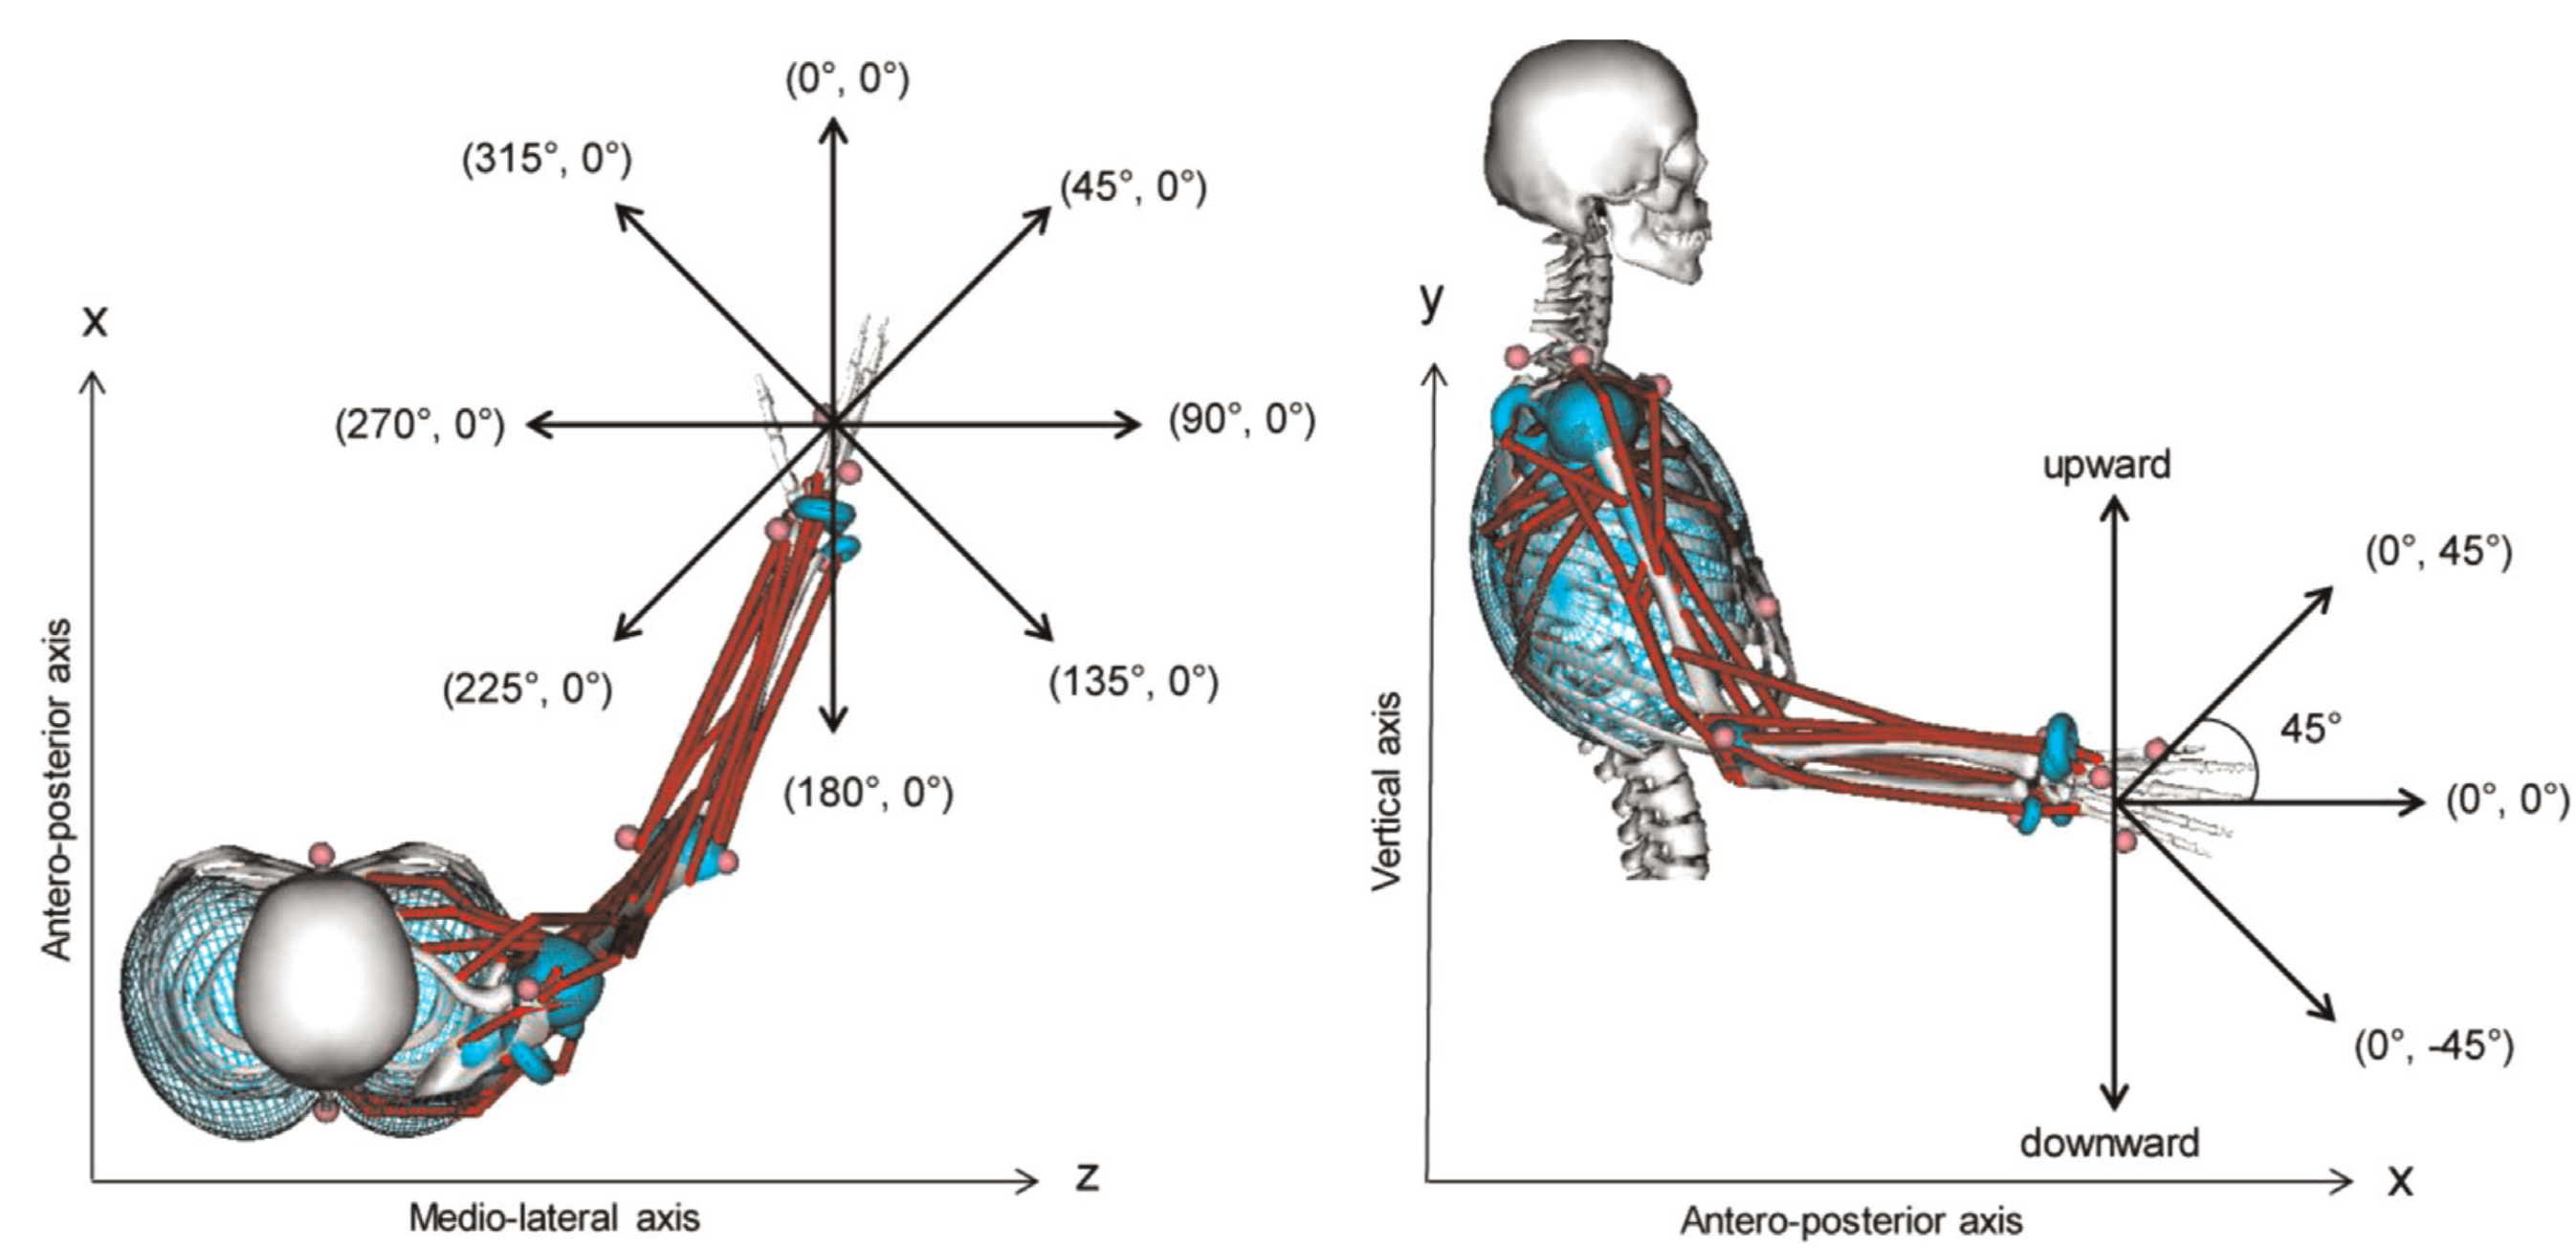
\includegraphics[trim={0 0 0 0},clip,width=0.9\linewidth]{img/chapter_1/axis_hernandez_rezzoug.png}
    \caption{This figure illustrates the 26 force directions employed in (\cite{rezzougUpperLimbIsometricForce2021b}) and (\cite{hernandezIsometricForceCapabilities2015}), defined by combinations of azimuth and elevation angles. The left panel depicts the azimuth angles, while the right panel shows the elevation angles. (Images adapted from (\cite{hernandezIsometricForceCapabilities2015})).}
    \label{fig:rezzoug_hernandez_directions_}
\end{figure}

From the 26 defined directions of force, pairs of opposing directions (pushing-pulling) were randomly selected. This ensured participants focused on a single line of action for two successive measurements, exerting force in opposite directions. The workspace axes were aligned with the Cartesian force space, with the origin at the force/torque sensor. The force x-axis corresponded to the normal of the coronal plane, the y-axis to the normal of the transverse plane, and the z-axis to the normal of the sagittal plane.

A white arrow on the screen indicated the target direction for force exertion, while a red arrow of fixed length represented the real-time direction of the exerted force. A gauge on the left side of the screen displayed the current force amplitude with a red fill. Its maximum value was set to 1000 Newtons, a limit that, although unattainable for participants, encouraged them to exert maximal forces.

\begin{figure}[!htb]
    \centering
    \captionsetup{justification=centering}
        \centering
        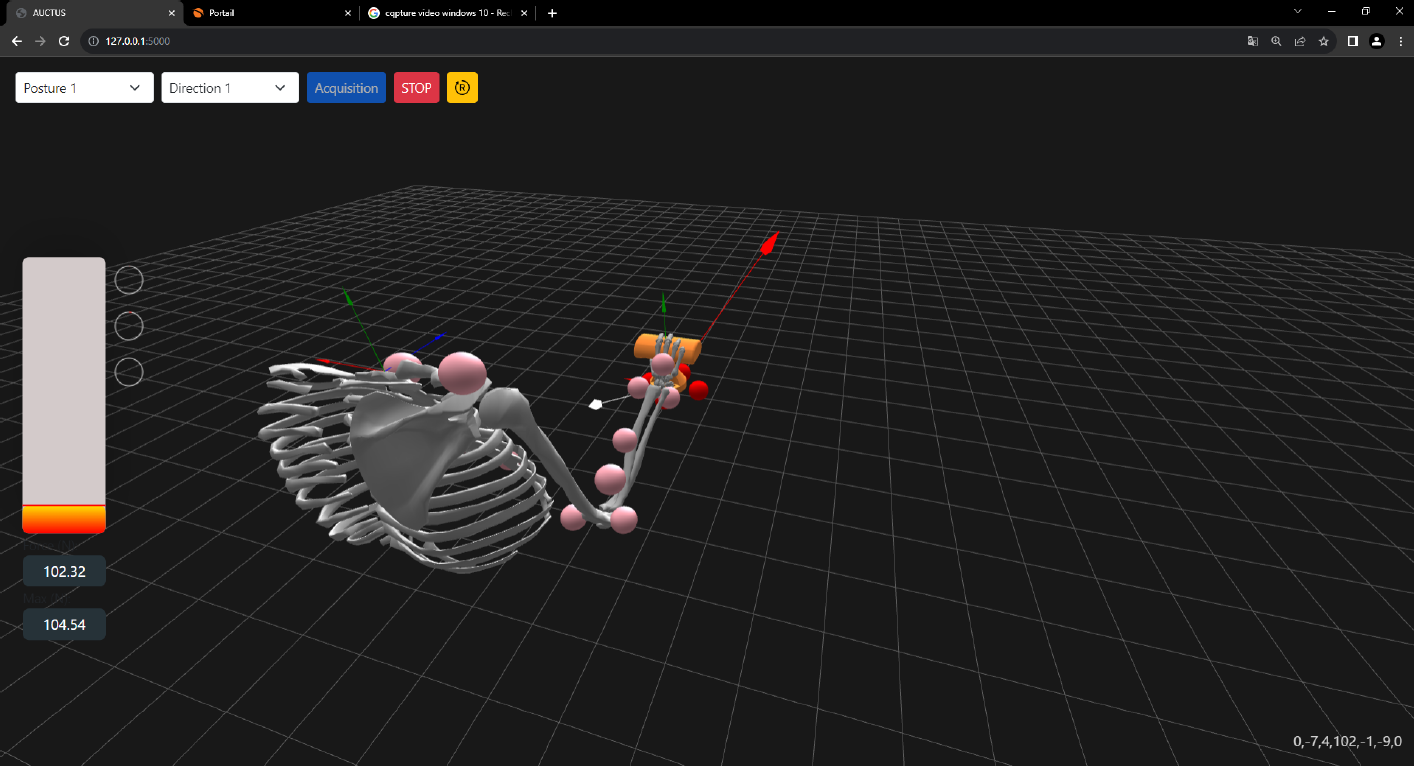
\includegraphics[trim={0 50 200 40}, clip, width=0.7\linewidth]{img/chapter_5/interface_2.png}
    \caption{Visual interface displaying the target force direction (white arrow), exerted force direction (red arrow), and force amplitude (gauge and as well as current and maximal value below).}
    \label{fig:interface_2}
\end{figure}


\subsection{Accounting for factors influencing a MVIC}

As described in Chapter \ref{chapter:1}, multiple factors influence the quality of a MVIC, such as respiration (\cite{leeComparisonMaximumVoluntary2016}), perceived fatigue (\cite{roseFatigueRecoveryStatic2014}), body posture (\cite{watanabeShortTermReliabilityGrip2005}), and circadian rhythm (\cite{jasperCircadianVariationsKinematics2009}).

Accordingly, we followed the recommendations and results from the above-mentioned articles. For instance, participants were asked to choose two 3-hour timeslots for the experiment within the same timeframe (morning or afternoon). To standardize respiration, individuals were instructed to inhale deeply before each MVIC and exert maximal force during exhalation. Although a standing posture might be more relevant for industrial collaborative tasks with a cobot, a sitting position was used in this study, as previous research (\cite{watanabeShortTermReliabilityGrip2005}) found no significant differences between sitting and standing for hand maximal forces.

As the experiment occurred in two sessions with more than 52 MVICs within each, physical as well as perceived fatigue may have occurred. To account for general muscle fatigue and ensure adequate recuperation between sessions, they were separated by at least three days. While physical fatigue was mitigated through 2-minute (minimum) rest periods between measurements (\cite{perdeauxInvestigatingRoleShoulder2010}), mental fatigue was addressed subjectively. Motivational verbal encouragement was provided during each measurement and also within rest periods. Additionally, when the experimenter noticed general fatigue, verbal exchanges to promote social interaction were favored to make the experiment less demanding and offer the participant less repetitive resting moments.

\subsection{Upper-limb postures of reference}
Four upper-limb postures were considered and are noted P1, P2, P3 and P4. This number accounts for the experimental difficulties of collecting 26 maximal isometric force exertions in a single posture. Based on Stanford's upper-limb musculoskeletal model (\cite{holzbaurModelUpperExtremity2005}), these postures are defined in Table \ref{tab:posture_init} and presented in Figures \ref{fig:exp_pose1}, \ref{fig:exp_pose2}, \ref{fig:exp_pose3} and \ref{fig:exp_pose4}.

\begin{table}[!ht]
    \centering
    \captionsetup{justification=centering}
    \resizebox{\textwidth}{!}{
    \begin{tabular}{|c||c|c|c|c|c|c|c|}
    \hline
    \textbf{Posture} & \makecell{\textbf{Elevation} \\ \textbf{angle}} & \makecell{\textbf{Shoulder} \\ \textbf{elevation}} & \makecell{\textbf{Shoulder} \\ \textbf{rotation}} & \makecell{\textbf{Elbow} \\ \textbf{flexion}} & \makecell{\textbf{Pronation} \\ \textbf{supination}} & \makecell{\textbf{Wrist} \\ \textbf{deviation}} & \makecell{\textbf{Wrist} \\ \textbf{flexion}} \\
    \hline
    P1 & $70$° & $20$° & $0$° & $90$° & $90$° & $0$° & $0$° \\ \hline
    P2 & $50$° & $65$° & $50$° & $70$° & $50$° & $0$° & $0$° \\ \hline
    P3 & $40$° & $68$° & $30$° & $30$° & $29$° & $0$° & $0$° \\ \hline
    P4 & $96$° & $65$° & $100$° & $33$° & $29$° & $0$° & $0$° \\
    \hline
    \end{tabular}}
    \caption{Joint configuration values (in degrees) for each considered posture in right upper-limb musculoskeletal model (\cite{holzbaurModelUpperExtremity2005}).}
    \label{tab:posture_init}
\end{table}

\begin{figure}[!htb]
    \centering
    \captionsetup{justification=centering}
    \begin{minipage}{0.3\linewidth}
        \centering
        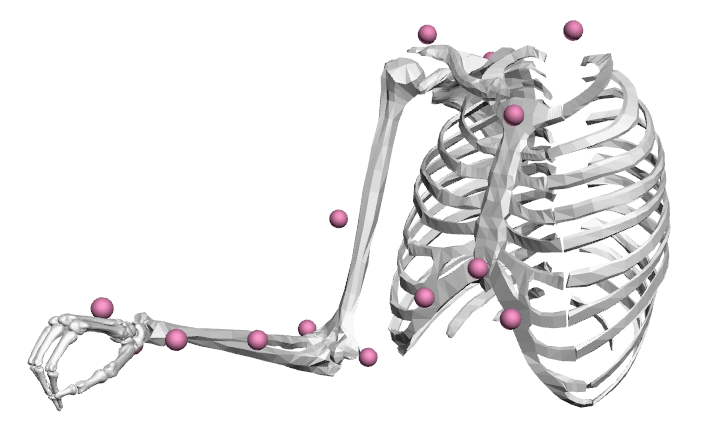
\includegraphics[trim={0 0 0 0}, clip, width=1\linewidth]{img/chapter_5/posture1_3D.png}
    \end{minipage}
    \hfill
    \begin{minipage}{0.3\linewidth}
        \captionsetup{justification=centering}
        \centering
        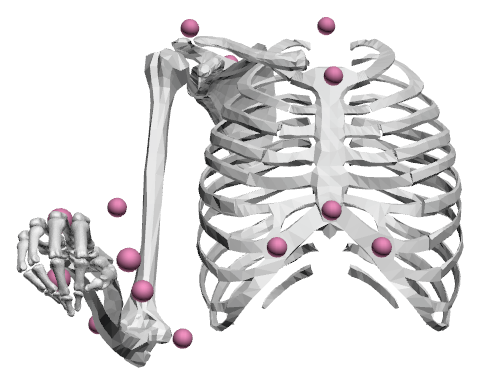
\includegraphics[trim={0 0 0 0}, clip, width=0.75\linewidth]{img/chapter_5/posture1_coronal.png}
    \end{minipage}
    \hfill
    \begin{minipage}{0.3\linewidth}
        \captionsetup{justification=centering}
        \centering
        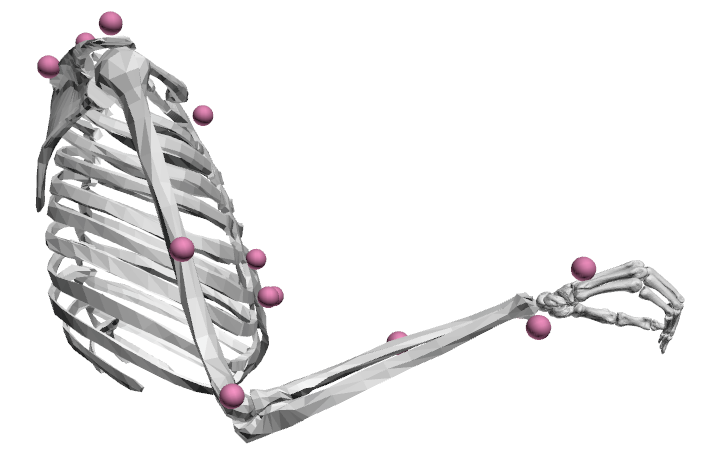
\includegraphics[trim={0 0 0 0}, clip, width=0.9\linewidth]{img/chapter_5/posture1_sagittal.png}
    \end{minipage}
    \caption{Visualization of posture P1 using Stanford's upper-limb model.}
    \label{fig:exp_pose1}
\end{figure}

\begin{figure}[!htb]
    \centering
    \captionsetup{justification=centering}
    \begin{minipage}{0.3\linewidth}
        \centering
        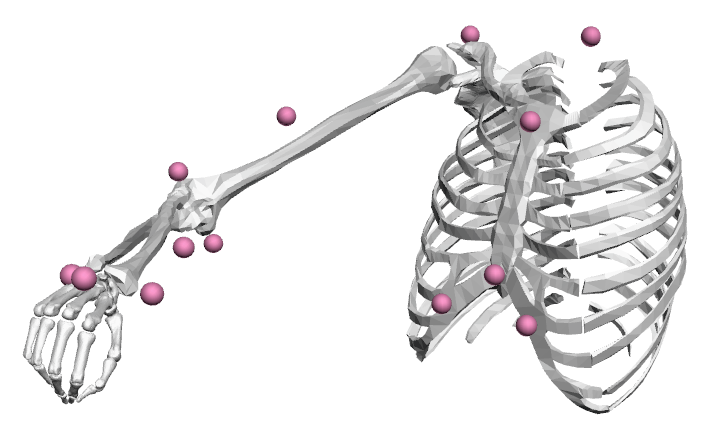
\includegraphics[trim={0 0 0 0}, clip, width=1\linewidth]{img/chapter_5/posture2_3D.png}
    \end{minipage}
    \hfill
    \begin{minipage}{0.3\linewidth}
        \captionsetup{justification=centering}
        \centering
        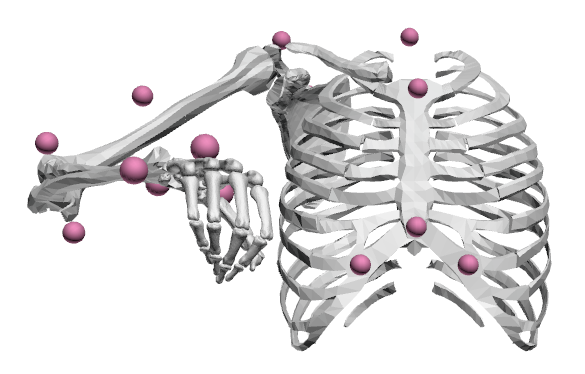
\includegraphics[trim={0 0 0 0}, clip, width=0.95\linewidth]{img/chapter_5/posture2_coronal.png}
    \end{minipage}
    \hfill
    \begin{minipage}{0.3\linewidth}
        \captionsetup{justification=centering}
        \centering
        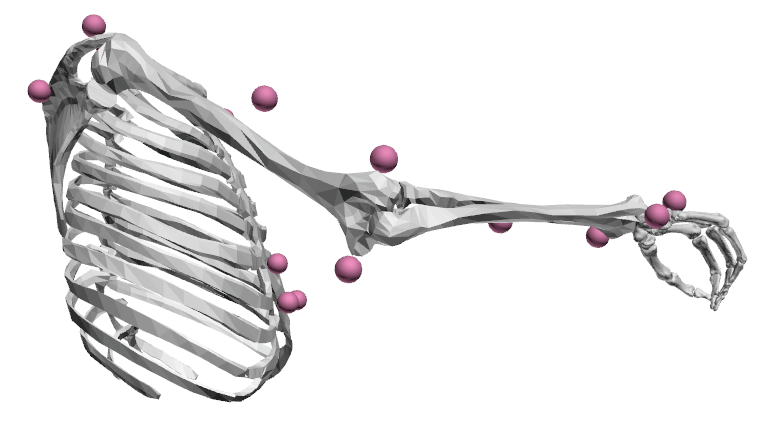
\includegraphics[trim={0 0 0 0}, clip, width=0.9\linewidth]{img/chapter_5/posture2_sagittal.png}
    \end{minipage}
    \caption{Visualization of posture P2 using Stanford's upper-limb model.}
    \label{fig:exp_pose2}
\end{figure}


\begin{figure}[!htb]
    \centering
    \captionsetup{justification=centering}
    \begin{minipage}{0.3\linewidth}
        \centering
        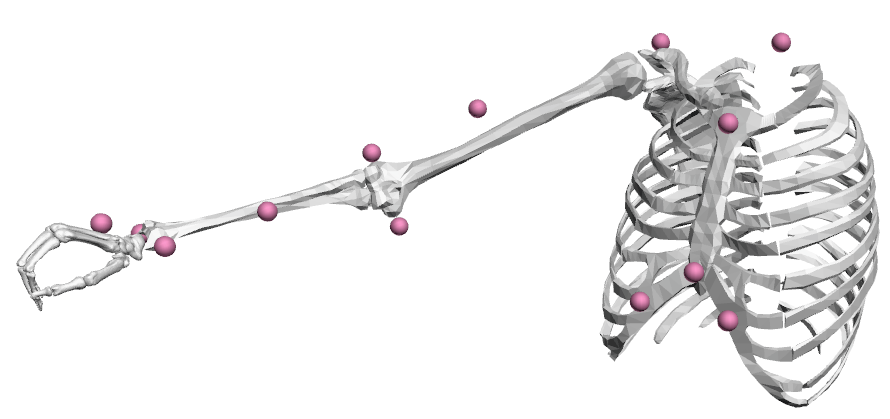
\includegraphics[trim={0 0 0 0}, clip, width=1\linewidth]{img/chapter_5/posture3_3D.png}
    \end{minipage}
    \hfill
    \begin{minipage}{0.3\linewidth}
        \captionsetup{justification=centering}
        \centering
        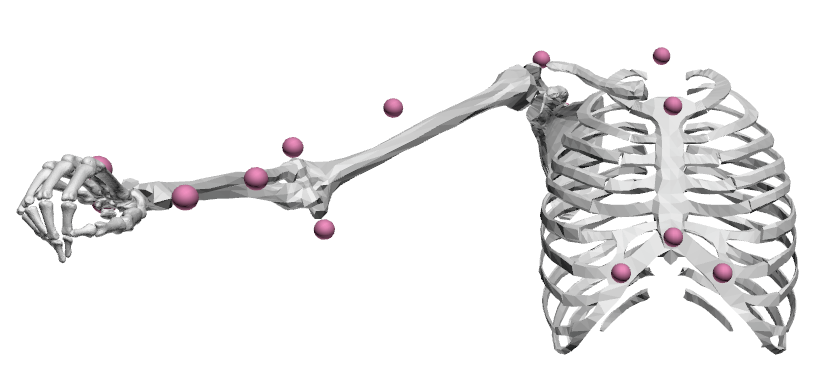
\includegraphics[trim={0 0 0 0}, clip, width=1\linewidth]{img/chapter_5/posture3_coronal.png}
    \end{minipage}
    \hfill
    \begin{minipage}{0.3\linewidth}
        \captionsetup{justification=centering}
        \centering
        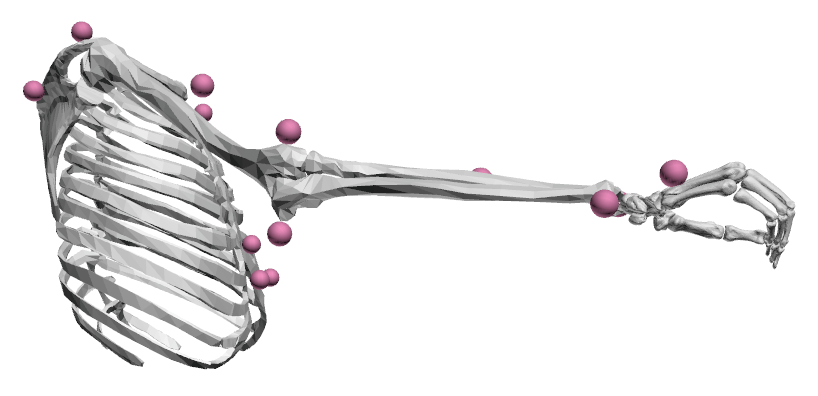
\includegraphics[trim={0 0 0 0}, clip, width=0.9\linewidth]{img/chapter_5/posture3_sagittal.png}
    \end{minipage}
    \caption{Visualization of posture P3 using Stanford's upper-limb model.}
    \label{fig:exp_pose3}
\end{figure}

\begin{figure}[!htb]
    \centering
    \captionsetup{justification=centering}
    \begin{minipage}{0.3\linewidth}
        \centering
        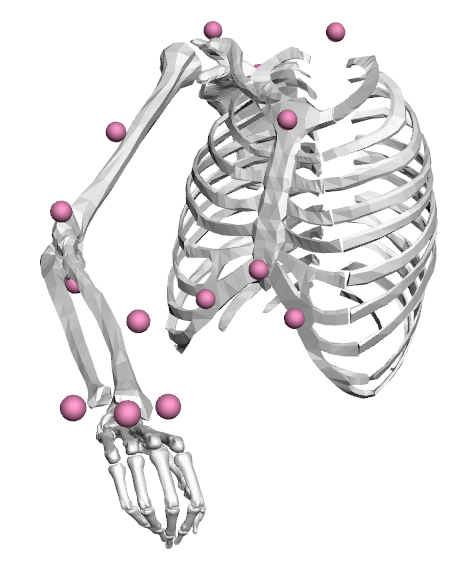
\includegraphics[trim={0 0 0 0}, clip, width=0.7\linewidth]{img/chapter_5/posture4_3D.png}
    \end{minipage}
    \hfill
    \begin{minipage}{0.3\linewidth}
        \captionsetup{justification=centering}
        \centering
        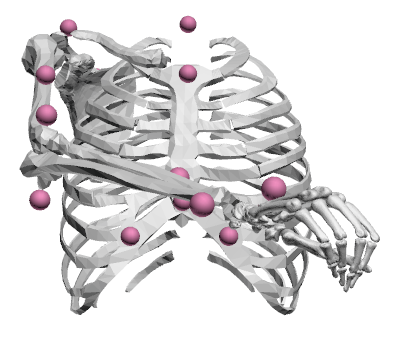
\includegraphics[trim={0 0 0 0}, clip, width=0.65\linewidth]{img/chapter_5/posture4_coronal.png}
    \end{minipage}
    \hfill
    \begin{minipage}{0.3\linewidth}
        \captionsetup{justification=centering}
        \centering
        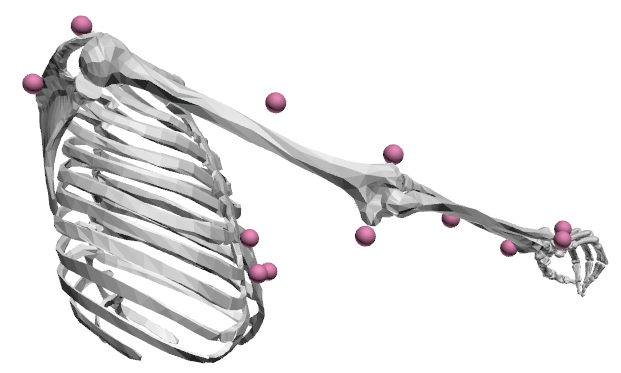
\includegraphics[trim={0 0 0 0}, clip, width=0.9\linewidth]{img/chapter_5/posture4_sagittal.png}
    \end{minipage}
    \caption{Visualization of posture P4 using Stanford's upper-limb model.}
    \label{fig:exp_pose4}
\end{figure}

\subsection{Proprioceptive placement of the upper limb}

Each of the four upper-limb postures, while defined for the joint coordinates of a musculoskeletal model, must be replicated by a participant, since no physical constraints on the right upper limb were used in this experiment. Also, since we want to compute \emph{in silico} force feasible sets at the hand of the individual, we needed to determine the participant's joint configuration during each MVIC. To achieve this, we used a proprioceptive approach based on real-time visual feedback of 14 reflective markers placed on the participant's right upper limb, trunk, and back of the head, as described below.

An optoelectronic system (OptiTrack) with 14 reflective markers (9mm diameter) was used to measure the individual's posture. The markers were placed on the skin of the right arm and torso using hypoallergenic double-sided adhesive. Marker positions were recorded at 100 Hz and filtered to reduce noise.

\begin{figure}[!htb]
    \centering
    \captionsetup{justification=centering}
    \begin{minipage}{0.59\linewidth}
        \centering
        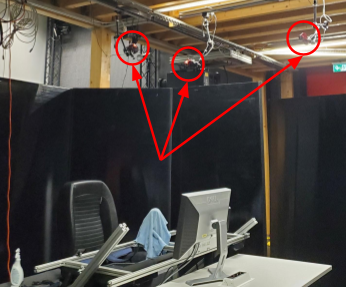
\includegraphics[clip, width=1\linewidth]{img/chapter_5/motion_capture_01.png}
    \end{minipage}
    \hfill
    \begin{minipage}{0.4\linewidth}
        \centering
        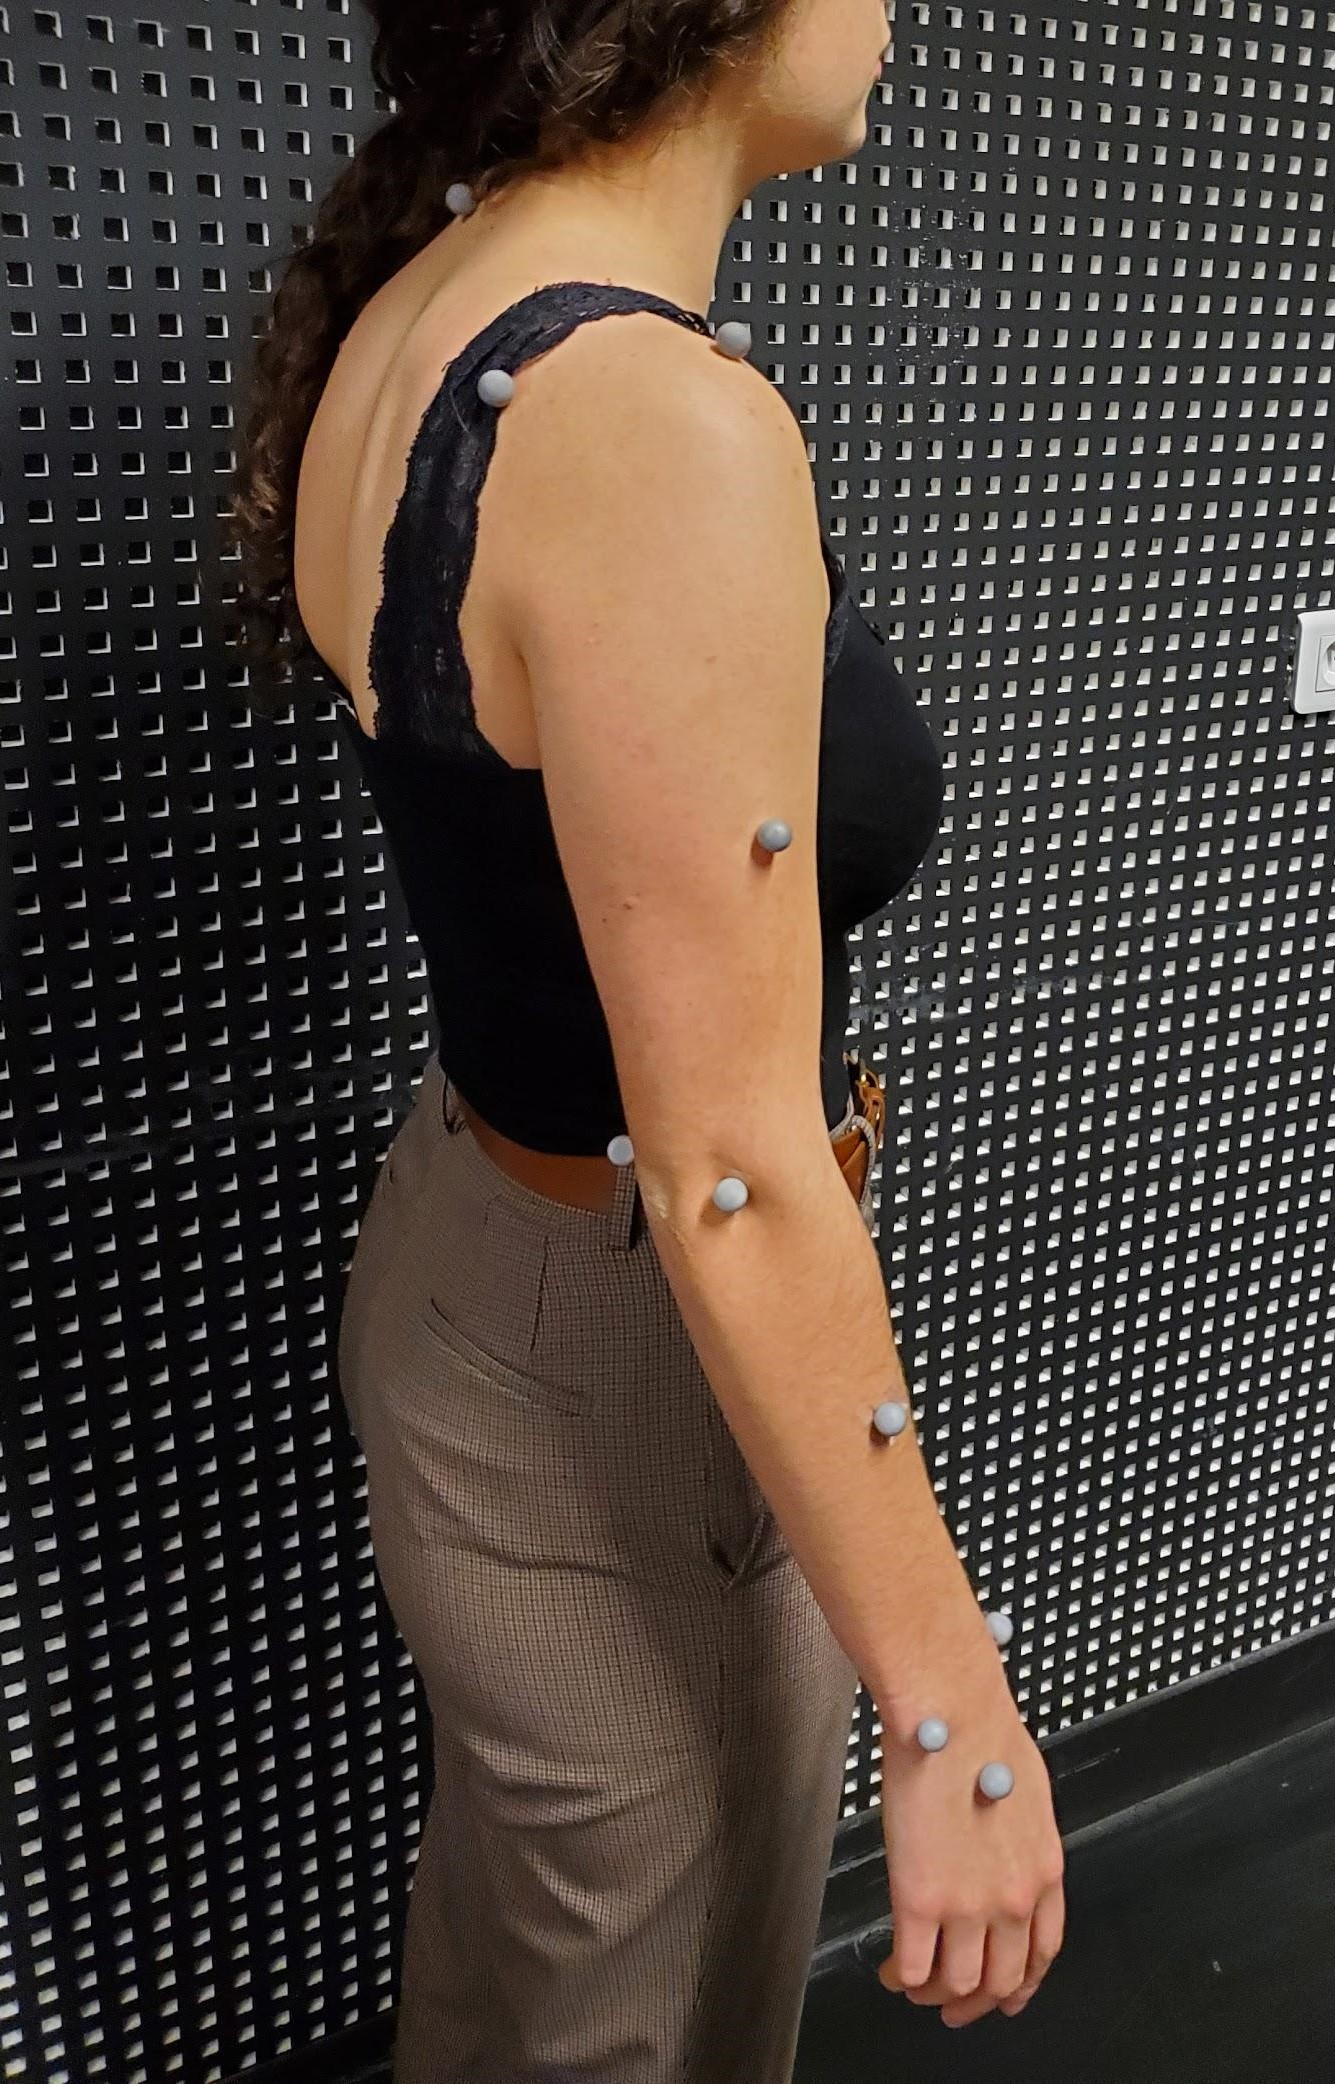
\includegraphics[clip,width=0.785\linewidth]{img/chapter_5/markers_02.jpg}
    \end{minipage}
    \caption{On the left: the placement of motion-capture cameras ensured the visibility of reflective markers in most directions. On the right: placement of the markers on the upper limb skin.}
    \label{fig:motion_capture}
\end{figure}

Because the upper limb was not physically constrained, a real-time visual interface was developed to help the participant maintain a constant posture throughout the experiment. This 3D interface displayed the participant's upper-limb marker positions (red) and the target marker positions (pink) on a scaled musculoskeletal model (Fig. \ref{fig:interface_1}). This allowed the participant to assess in real-time whether their current posture matched the target. However, maintaining a fixed posture while exerting maximal force could be challenging. Therefore, the experimenter visually monitored the participant's posture throughout the experiment.

\begin{figure}[!htb]
    \centering
    \captionsetup{justification=centering}
    \begin{minipage}{0.49\linewidth}
        \centering
        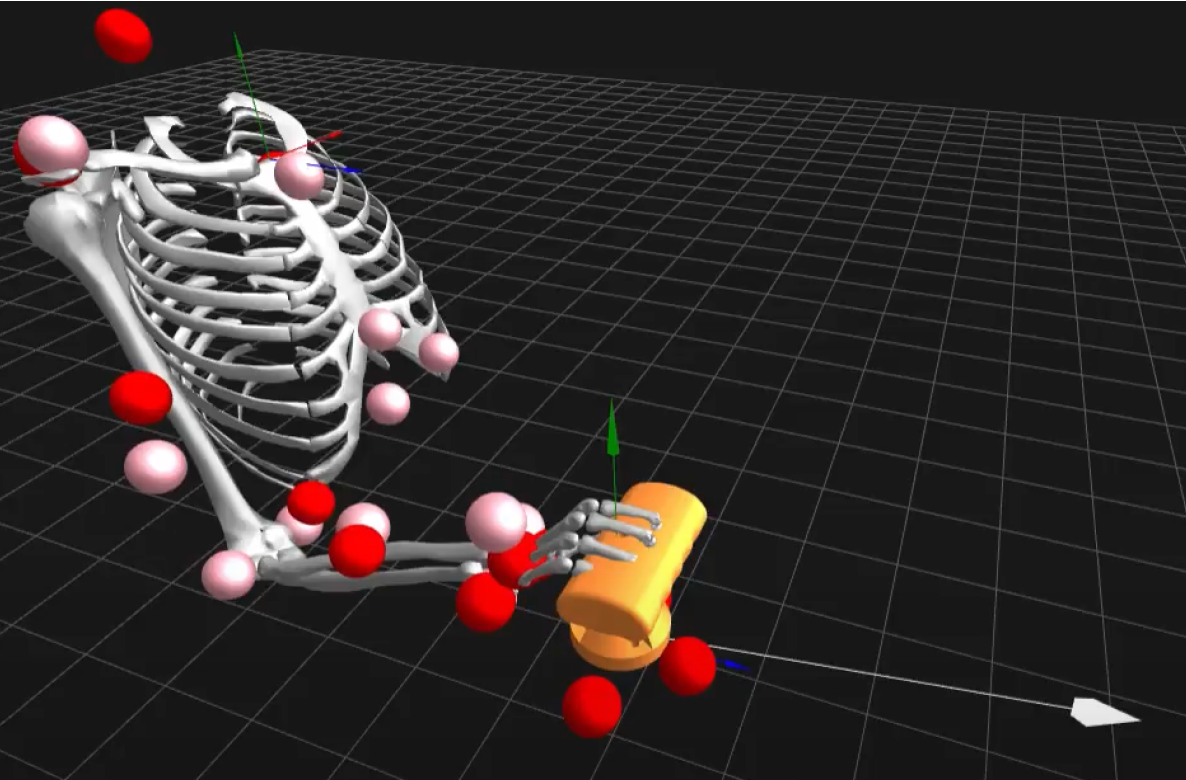
\includegraphics[trim={0 0 0 0}, clip, width=1\linewidth]{img/chapter_5/interface_1.png}
    \end{minipage}
    \hfill
    \begin{minipage}{0.49\linewidth}
        \centering
        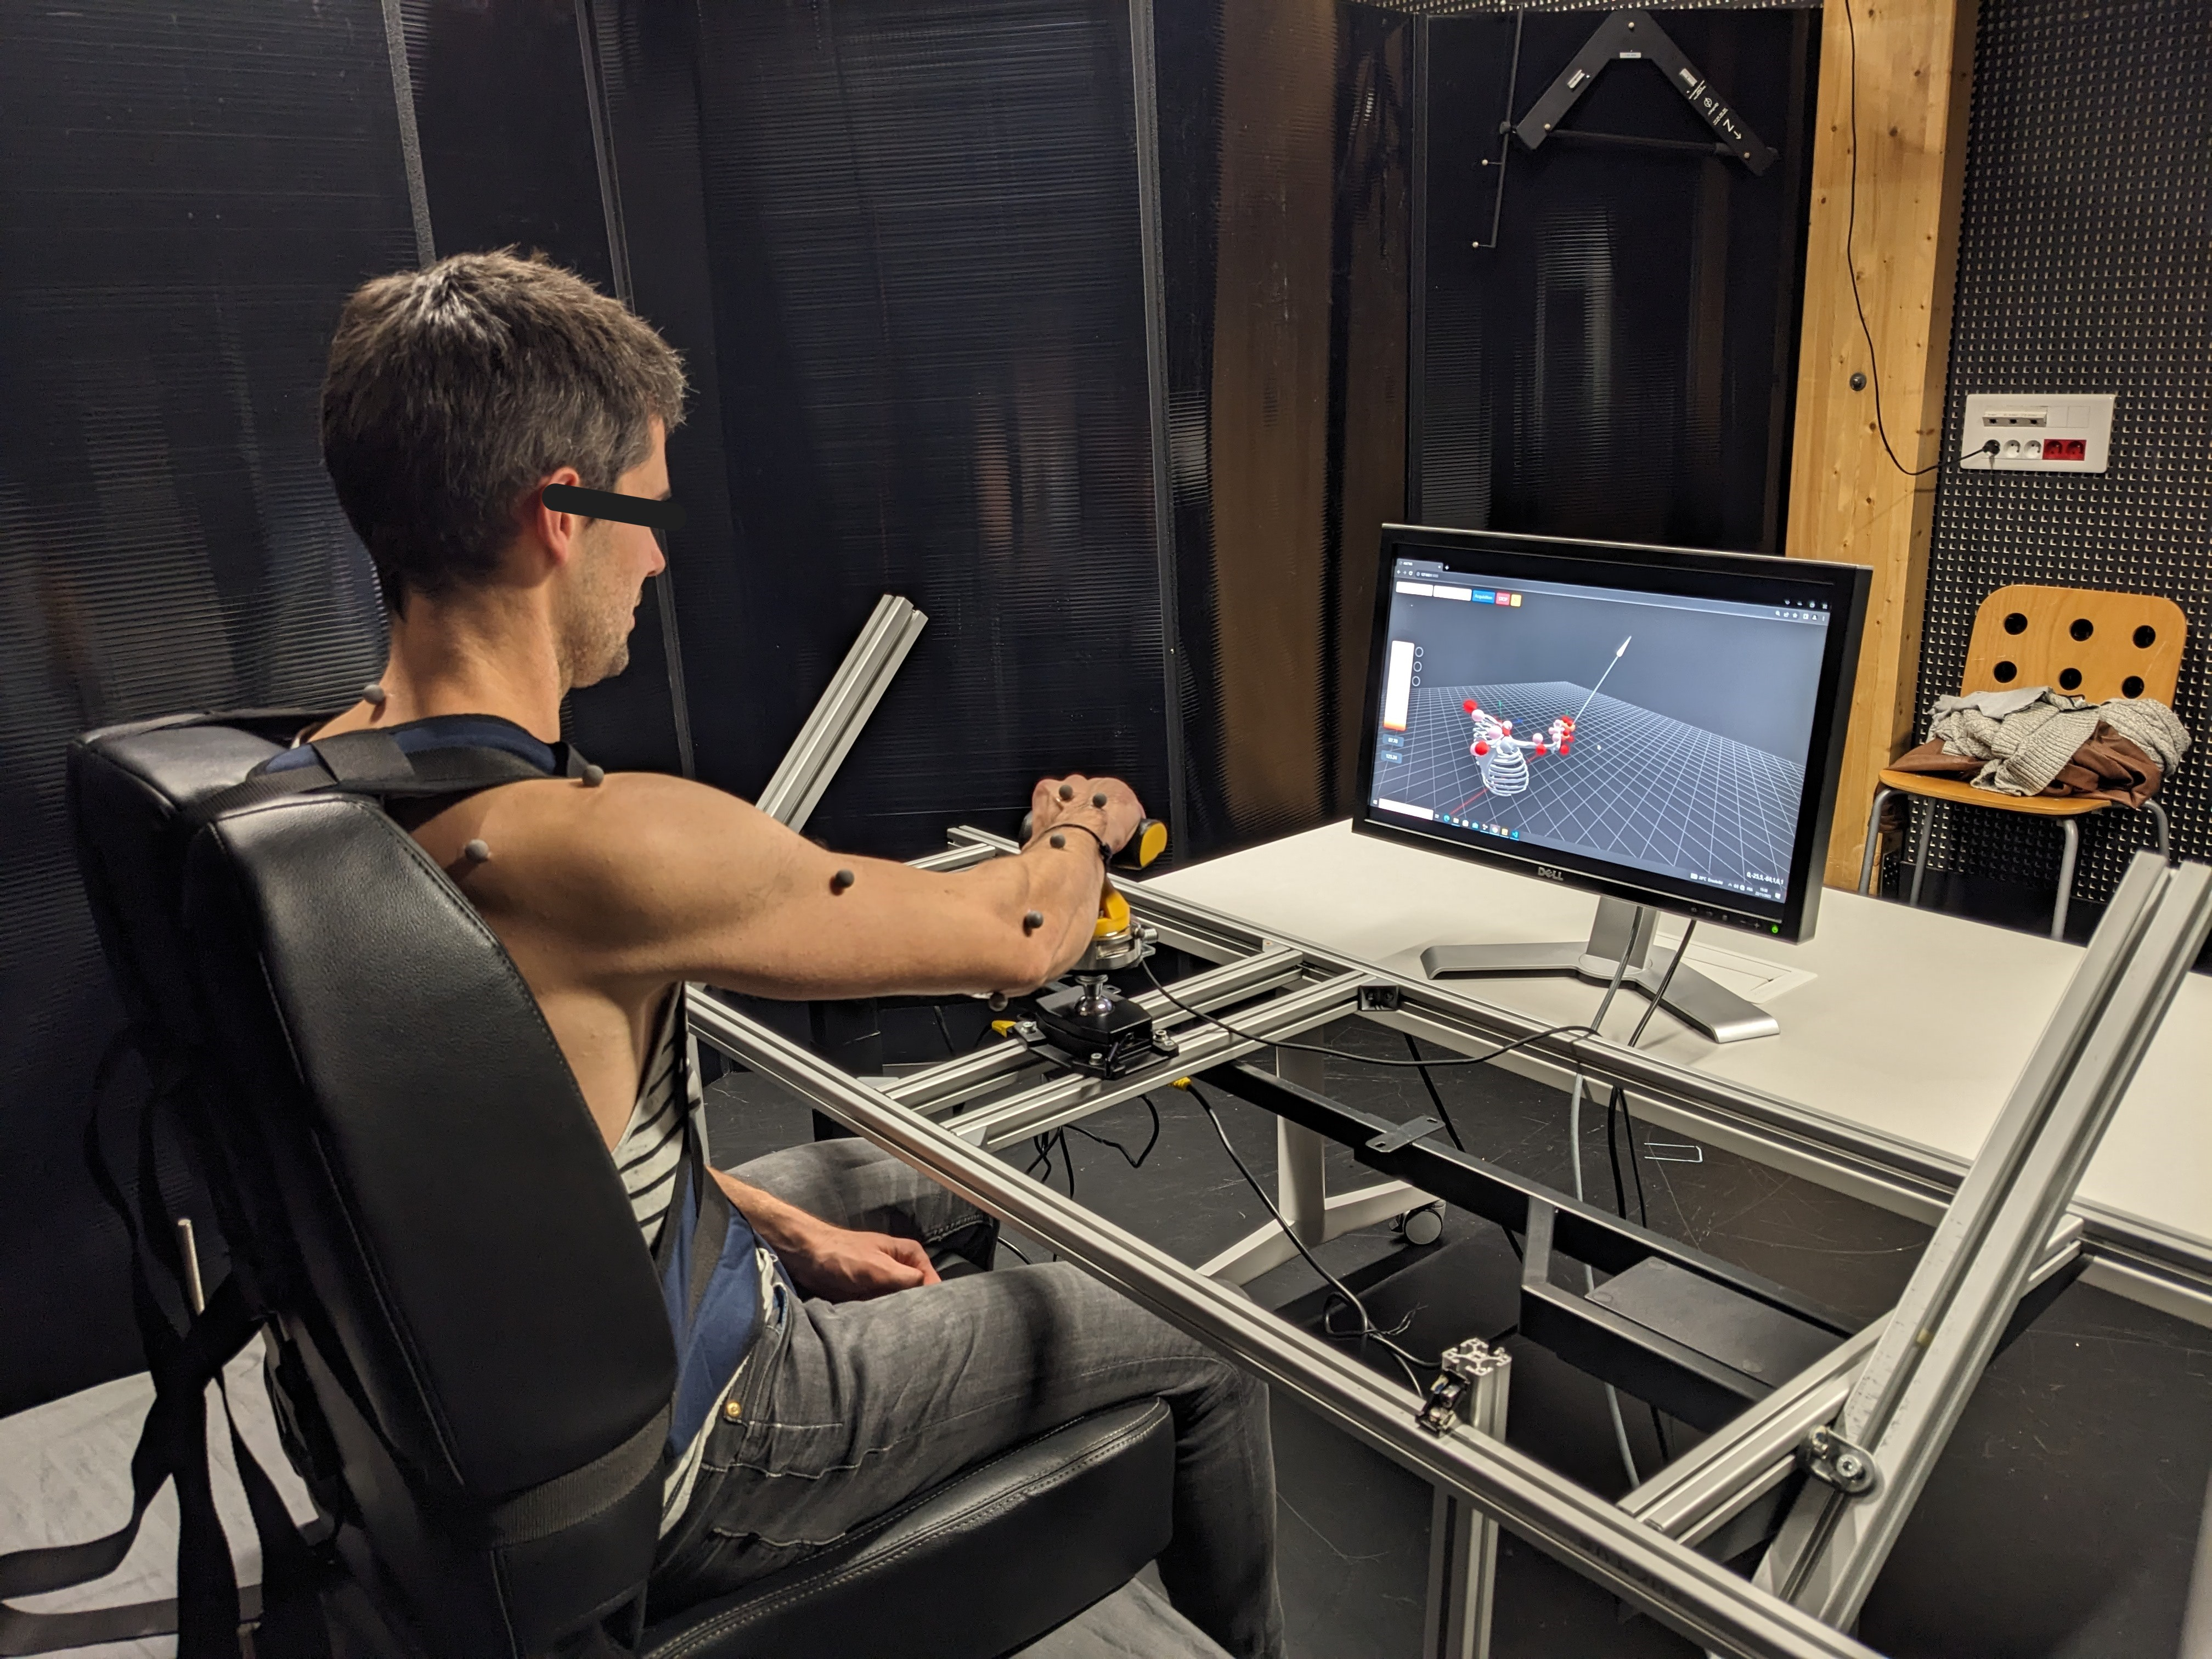
\includegraphics[trim={0 0 0 60}, clip, width=0.9\linewidth]{img/chapter_5/measure_03.jpg}
    \end{minipage}
    \caption{3D interface providing visual feedback of the participant's marker positions (red) relative to the target posture (pink) on a scaled musculoskeletal model.}
    \label{fig:interface_1}
\end{figure}

\subsection{Experimental Protocol}

The experiment occurred at INRIA of University of Bordeaux. For each participant, two 3-hour timeslots were planned. Each session consisted of measuring maximal force exertions in 26 different directions for two different right upper limb postures. The order of the postures was randomized for each participant, as shown in Table \ref{tab:posture_subjects_passation}. Only one participant had to return for another session due to technical difficulties that occurred during the first session, making it too long.

\begin{table}[!ht]
    % \scriptsize
    \centering
    \captionsetup{justification=centering}
    \begin{tabular}{|c|c|c|c|}
        \hline
        \textbf{Subject} & \makecell{\textbf{Postures in} \\ \textbf{session 1}} & \makecell{\textbf{Postures in} \\ \textbf{session 2}} & \makecell{\textbf{Postures in} \\ \textbf{session 3}} \\
        \hline
        S1 & P4, P3 & P2, P1 & / \\ \hline
        S2 & P4, P1 & P3, P2 & / \\ \hline
        S3 & P2, P3 & P1, P4 & / \\ \hline
        S4 & P3, P1 & P4, P2 & / \\ \hline
        S5 & P3, P2 & P4, P1 & / \\ \hline
        S6 & P2, P3 & P1, P4 & / \\ \hline
        S7 & P2, P1 & P4, P3 & / \\ \hline
        S8 & P2, P3 & P1, P4 & / \\ \hline
        S9 & P2, P1 & P3, P4 & / \\ \hline
        S10 & P1 & P4, P3 & P2 \\ \hline
    \end{tabular}
    \caption{Posture order within each required session for each participant.}
    \label{tab:posture_subjects_passation}
\end{table}

The first session included the collection of anthropometric data, such as mass, height, sports activities, age, and dominant hand. Any volunteer who had an upper limb, back, or torso muscular pathology or injury (sprain, tendinitis, strain, tear, etc.) in the previous 6 months was not considered for the experiment. This also applied to orthopedic pathologies, musculoskeletal and neuromuscular disorders.

Both sessions started with the placement of reflective markers on the upper limb, torso, and back. The participant was then asked to assume a T-pose to scale a generic musculoskeletal model to their body geometry. This was followed by a 10-minute exercise routine, including stretching and rotations of each upper limb joint up to their maximal range at various speeds. The participant was then positioned in the seat and secured with shoulder straps to prevent shoulder movement.

A computer screen in front of the participant displayed their current marker positions (red) and the target marker positions (pink) corresponding to the first posture of the session. The participant could then adjust their upper limb posture to align the red markers with the pink ones. The force/torque sensor was then positioned at the participant's hand by adjusting the table height and the handle position and orientation. After this process, all physical components of the setup were fixed and secured. The participant performed a few submaximal force exertions to become familiar with the posture and practice exerting force in the required directions. Five maximal force exertions were then performed in randomly chosen directions from the defined set of force directions, with a 2-minute rest between each. Measurements were collected when the participant felt sufficiently confident to start the experiment.

Every force exertion was codified and lasted at least 5 seconds, as described in (\cite{perdeauxInvestigatingRoleShoulder2010}; \cite{choppFeasibilityObtainingMultiple2010}): 2 seconds to attain the maximal force in the required direction; 3 seconds to maintain the force; and 1 second to decrease the exerted force. Between exertions, the participant rested for a minimum of two minutes to avoid muscle fatigue (\cite{chaffinOccupationalBiomechanics2006}; \cite{perdeauxInvestigatingRoleShoulder2010}; \cite{choppFeasibilityObtainingMultiple2010}). As loud verbal encouragements have been shown to significantly influence the maximal force produced (\cite{jungEffectsInstructionVerbal1999}; \cite{johanssonRelationshipVerbalCommand1983a}), the experimenter actively encouraged each MVIC by loudly providing motivational words and phrases, such as `Allez !' (`Go!'), `Pousse !' (`Push!'), `Tu peux le faire !' (`You can do it!'), etc. These were inspired by the English standardized instruction set defined in (\cite{mathiowetzReliabilityValidityGrip1984a}). During the 2-minute rest period after each MVIC, the participant was asked to stretch their wrist and hydrate if needed. Brief feedback and encouragement were provided after each MVIC. All participants were allowed to repeat a MVIC if they felt they could perform it better.

When all force direction measurements for the first posture were completed, the participant was given a 15-minute rest period, during which their shoulder straps were removed so they could walk and stretch. During this time, the experimenter adjusted the setup for the next posture. Once the participant was ready, the same procedure was followed, starting with the participant being positioned in the chair, the straps secured, and the setup adjusted for the second posture.

Each session concluded with a stretching session (up to 20 minutes) and the provision of nutritious snacks.

\subsection{Ethical validation}
The target population mainly consists of asymptomatic young adults between the ages of 18 and 35. To be eligible for participation, individuals must meet the following inclusion criteria:

\begin{itemize}[noitemsep]
    \item Adult participants (aged 18-35 years) enrolled in a social security system;
    \item A Body Mass Index (BMI) within the normal range (20-30 kg/m²) as calculated using anthropometric data (height and weight) collected prior to engaging in the study;
    \item Participants must report engaging in a minimum of two hours of physical activity per week.
\end{itemize}

An individual was barred from the experiment if he was ineligible to participate according to articles L. 1121-5 to L. 1121-8 of the French public health code (which pertains to minors, protected adults, etc.)\footnote{The French public health code (\emph{Code de la santé publique}) is available at \url{https://www.legifrance.gouv.fr/codes/texte_lc/LEGITEXT000006072665/}.}, or if he had any of the following: no social security coverage; a musculoskeletal, cardiovascular, pulmonary, and/or metabolic disorder; a history of trauma or joint surgery reported in the last six months (at the shoulder, elbow, or wrist); or had not signed the informed consent form. The consent form includes a survey to assess eligibility criteria.

Three female and seven male participants between 21 and 32 years old were recruited for the experiment on a voluntary basis. Female participants' heights ranged from 1.65m to 1.68m, whereas male participants' heights ranged from 1.73m to 1.92m. All participants had a BMI between 20 and 28.

The experiment did not present safety hazards and was validated by INRIA's operational committee for the assessment of legal and ethical risks (COERLE\footnote{COERLE stands for \emph{Comité opérationnel d'évaluation des risques légaux et éthiques}.}). An informed consent form was signed and acknowledged by each participant

\section{Posture stability}
\label{sec:posture_stability}
For each maximal isometric force exertion trial in a specific posture, the participant had to maintain the required posture using visual feedback. This section assesses the extent to which participants achieved this.

For each direction of force exertion, marker positions and force/torque data were gathered simultaneously at 100 Hz and 230 Hz respectively. Force amplitude measurements showed that in general a participant reached their peak isometric force about 2 seconds after the trial starts and maintains it for about seconds, as a plateau can be observed within this timeframe for force amplitudes data. Therefore, only marker positions within this timeframe are considered for each measurement.

To determine the participant's posture, a scaling process was performed. Since the experiment involved two sessions, a musculoskeletal model based on Stanford's model (\cite{holzbaurModelUpperExtremity2005}) was scaled within OpenSim software (\cite{delpOpenSimOpenSourceSoftware2007}) using a static measurement recorded at the beginning of each session. Because there were two sessions, and marker placement might differ slightly between sessions, the scaled model markers were adjusted accordingly. Therefore, each participant had one scaled model, but two sets of corresponding marker positions (one for each session).

For each force measurement trial, the inverse kinematics tool in OpenSim was used to determine the posture. This process adjusts the joint configuration of the model to fit the model markers to the measured markers. As recommended by OpenSim software developers, the root mean square error (RMSE) between the marker placements of the scaled model and the measured marker positions should be less than 2 cm. All inverse kinematic processes respected this constraint.

To assess posture maintenance, we calculated the mean, minimum, and maximum values for each joint coordinate retrieved from inverse kinematics of each maximal force exertion trial. Posture variability was then assessed by analyzing the joint coordinate data across all trials within a given posture. This included calculating the mean and standard deviation of the mean joint coordinate values for each trial (Table \ref{tab:posture_stability}; Fig. \ref{fig:example_pos_489_elbow_flexion}), as well as the overall minimum and maximum values across all trials (Table \ref{tab:posture_stability_ranges}).

\begin{table}[!ht]
    \scriptsize
    \centering
    \resizebox{\textwidth}{!}{
    \begin{tabular}{|c|c||c|c|c|c|c|c|c|c|c|c|}
    \hline
    \textbf{Subject} & \textbf{Posture} & \makecell{\textbf{Trunk} \\ \textbf{rotation} $x$} & \makecell{\textbf{Trunk} \\ \textbf{rotation} $y$} & \makecell{\textbf{Trunk} \\ \textbf{rotation} $z$} & \makecell{\textbf{Elevation} \\ \textbf{angle}} & \makecell{\textbf{Shoulder} \\ \textbf{elevation}} & \makecell{\textbf{Shoulder} \\ \textbf{rotation}} & \makecell{\textbf{Elbow} \\\textbf{flexion}} & \makecell{\textbf{Pronation} \\ \textbf{supination}} & \makecell{\textbf{Wrist} \\ \textbf{deviation}} & \makecell{\textbf{Wrist} \\ \textbf{flexion}} \\
    \hline
    \multirow{4}{*}{S1} & P1 & $[-5, 5]$ & $[-9, 2]$ & $[-9, 0]$ & $[42, 68]$ & $[29, 55]$ & $[3, 32]$ & $[52, 96]$ & $[61, 86]$ & $[-15, 19]$ & $[-35, 5]$ \\
     & P2 & $[-9, -2]$ & $[-6, 5]$ & $[-9, -2]$ & $[43, 69]$ & $[57, 74]$ & $[25, 48]$ & $[54, 82]$ & $[49, 69]$ & $[-4, 12]$ & $[-27, 14]$ \\
     & P3 & $[-7, 0]$ & $[-8, 2]$ & $[-9, -2]$ & $[28, 50]$ & $[58, 76]$ & $[-6, 25]$ & $[29, 66]$ & $[68, 87]$ & $[-4, 17]$ & $[-23, 17]$ \\
     & P4 & $[-9, -5]$ & $[4, 9]$ & $[-9, -6]$ & $[74, 97]$ & $[57, 75]$ & $[43, 74]$ & $[34, 67]$ & $[62, 88]$ & $[-5, 16]$ & $[-26, 21]$ \\
    \hline
    \hline
    \multirow{4}{*}{S2} & P1 & $[-2, 7]$ & $[-2, 6]$ & $[-7, 2]$ & $[37, 68]$ & $[28, 62]$ & $[-8, 23]$ & $[80, 113]$ & $[59, 89]$ & $[-14, 16]$ & $[-34, 22]$ \\
     & P2 & $[-9, -1]$ & $[-5, 8]$ & $[-7, 4]$ & $[32, 53]$ & $[52, 76]$ & $[27, 59]$ & $[70, 90]$ & $[57, 84]$ & $[2, 19]$ & $[-30, 15]$ \\
     & P3 & $[-9, -1]$ & $[-3, 6]$ & $[-8, 1]$ & $[24, 38]$ & $[53, 73]$ & $[7, 39]$ & $[61, 78]$ & $[57, 88]$ & $[0, 20]$ & $[-30, 9]$ \\
     & P4 & $[-9, 1]$ & $[2, 9]$ & $[-8, -1]$ & $[58, 75]$ & $[59, 79]$ & $[44, 71]$ & $[55, 75]$ & $[35, 81]$ & $[11, 21]$ & $[-26, 10]$ \\
    \hline
    \hline
    \multirow{4}{*}{S3} & P1 & $[2, 8]$ & $[-8, -1]$ & $[-9, -4]$ & $[50, 75]$ & $[40, 54]$ & $[-3, 12]$ & $[65, 84]$ & $[51, 85]$ & $[-8, 16]$ & $[-30, 0]$ \\
     & P2 & $[-2, 8]$ & $[-7, 7]$ & $[-9, -7]$ & $[43, 65]$ & $[66, 84]$ & $[31, 56]$ & $[52, 72]$ & $[2, 36]$ & $[-5, 17]$ & $[-23, 13]$ \\
     & P3 & $[-1, 8]$ & $[-5, 6]$ & $[-9, -7]$ & $[23, 50]$ & $[67, 83]$ & $[-7, 29]$ & $[18, 48]$ & $[10, 61]$ & $[-8, 15]$ & $[-31, 2]$ \\
     & P4 & $[-5, 8]$ & $[2, 9]$ & $[-9, -1]$ & $[60, 100]$ & $[55, 75]$ & $[41, 67]$ & $[25, 72]$ & $[45, 77]$ & $[-4, 20]$ & $[-29, 1]$ \\
    \hline
    \hline
    \multirow{4}{*}{S4} & P1 & $[-4, 8]$ & $[-8, 0]$ & $[-7, 8]$ & $[28, 59]$ & $[27, 50]$ & $[7, 46]$ & $[62, 112]$ & $[10, 89]$ & $[-12, 18]$ & $[-32, 22]$ \\
     & P2 & $[-7, 8]$ & $[-9, 4]$ & $[-8, 7]$ & $[41, 71]$ & $[55, 83]$ & $[28, 61]$ & $[33, 81]$ & $[49, 75]$ & $[-9, 7]$ & $[-28, 20]$ \\
     & P3 & $[-9, 7]$ & $[-3, 6]$ & $[-7, 2]$ & $[28, 55]$ & $[53, 81]$ & $[-1, 39]$ & $[19, 74]$ & $[59, 88]$ & $[-5, 19]$ & $[-29, 20]$ \\
     & P4 & $[-9, 9]$ & $[-9, 8]$ & $[-8, 9]$ & $[60, 94]$ & $[58, 78]$ & $[52, 83]$ & $[19, 73]$ & $[41, 77]$ & $[-7, 20]$ & $[-22, 18]$ \\
    \hline
    \hline
    \multirow{4}{*}{S5} & P1 & $[-2, 8]$ & $[-4, 3]$ & $[-8, 4]$ & $[26, 70]$ & $[19, 38]$ & $[-3, 15]$ & $[85, 114]$ & $[84, 89]$ & $[-4, 18]$ & $[-30, 16]$ \\
     & P2 & $[-9, 6]$ & $[-2, 6]$ & $[-8, 4]$ & $[34, 59]$ & $[55, 87]$ & $[23, 51]$ & $[56, 88]$ & $[38, 70]$ & $[-6, 13]$ & $[-32, 10]$ \\
     & P3 & $[-8, 6]$ & $[-4, 7]$ & $[-6, 6]$ & $[15, 42]$ & $[49, 78]$ & $[-3, 28]$ & $[45, 77]$ & $[45, 77]$ & $[-11, 14]$ & $[-33, 17]$ \\
     & P4 & $[-9, 1]$ & $[3, 9]$ & $[-9, -1]$ & $[60, 85]$ & $[61, 82]$ & $[48, 71]$ & $[46, 72]$ & $[47, 88]$ & $[2, 20]$ & $[-29, 13]$ \\
    \hline
    \hline
    \multirow{4}{*}{S6} & P1 & $[-9, 6]$ & $[-9, 9]$ & $[-9, -1]$ & $[29, 77]$ & $[26, 57]$ & $[-5, 32]$ & $[73, 106]$ & $[67, 90]$ & $[-9, 22]$ & $[-29, 32]$ \\
     & P2 & $[-9, 5]$ & $[-6, 6]$ & $[-4, 5]$ & $[34, 61]$ & $[58, 80]$ & $[33, 63]$ & $[63, 83]$ & $[34, 71]$ & $[0, 19]$ & $[-28, 27]$ \\
     & P3 & $[-9, 4]$ & $[-9, 9]$ & $[-6, 8]$ & $[8, 55]$ & $[44, 77]$ & $[5, 50]$ & $[25, 71]$ & $[39, 87]$ & $[-12, 22]$ & $[-33, 32]$ \\
     & P4 & $[-9, 1]$ & $[3, 9]$ & $[-9, 7]$ & $[60, 84]$ & $[47, 80]$ & $[39, 77]$ & $[46, 74]$ & $[46, 83]$ & $[-8, 20]$ & $[-29, 28]$ \\
    \hline
    \hline
    \multirow{4}{*}{S7} & P1 & $[2, 9]$ & $[-8, 1]$ & $[-1, 8]$ & $[-10, 44]$ & $[19, 40]$ & $[2, 20]$ & $[84, 120]$ & $[72, 88]$ & $[-11, 16]$ & $[-33, -3]$ \\
     & P2 & $[-9, 8]$ & $[-4, 9]$ & $[-4, 7]$ & $[33, 65]$ & $[56, 83]$ & $[22, 58]$ & $[46, 76]$ & $[41, 84]$ & $[5, 21]$ & $[-31, -6]$ \\
     & P3 & $[-4, 8]$ & $[-3, 9]$ & $[-3, 8]$ & $[9, 44]$ & $[61, 79]$ & $[8, 43]$ & $[33, 72]$ & $[57, 87]$ & $[0, 19]$ & $[-32, -2]$ \\
     & P4 & $[-9, 8]$ & $[3, 9]$ & $[-3, 8]$ & $[59, 82]$ & $[55, 80]$ & $[54, 82]$ & $[37, 72]$ & $[37, 86]$ & $[-2, 20]$ & $[-32, 1]$ \\
    \hline
    \hline
    \multirow{4}{*}{S8} & P1 & $[4, 9]$ & $[-3, 6]$ & $[0, 7]$ & $[20, 58]$ & $[20, 48]$ & $[-6, 11]$ & $[94, 116]$ & $[42, 83]$ & $[-13, 20]$ & $[-16, 32]$ \\
     & P2 & $[-5, 5]$ & $[-2, 9]$ & $[-4, 3]$ & $[23, 51]$ & $[51, 81]$ & $[19, 56]$ & $[76, 101]$ & $[-88, 81]$ & $[-14, 23]$ & $[-35, 30]$ \\
     & P3 & $[-4, 6]$ & $[0, 8]$ & $[-3, 5]$ & $[17, 42]$ & $[59, 75]$ & $[-11, 32]$ & $[19, 65]$ & $[51, 79]$ & $[-10, 16]$ & $[-15, 30]$ \\
     & P4 & $[-8, 6]$ & $[3, 9]$ & $[-5, 5]$ & $[56, 75]$ & $[51, 89]$ & $[45, 93]$ & $[55, 86]$ & $[13, 66]$ & $[-12, 20]$ & $[-30, 22]$ \\
    \hline
    \hline
    \multirow{4}{*}{S9} & P1 & $[-1, 7]$ & $[-6, 7]$ & $[-5, 4]$ & $[22, 68]$ & $[29, 53]$ & $[-2, 29]$ & $[70, 100]$ & $[61, 87]$ & $[-8, 14]$ & $[-29, 25]$ \\
     & P2 & $[-9, 3]$ & $[-4, 9]$ & $[-9, 3]$ & $[36, 64]$ & $[47, 73]$ & $[21, 56]$ & $[51, 82]$ & $[57, 82]$ & $[-4, 13]$ & $[-28, 12]$ \\
     & P3 & $[-7, 5]$ & $[2, 9]$ & $[-6, -2]$ & $[25, 42]$ & $[61, 76]$ & $[5, 28]$ & $[39, 66]$ & $[64, 88]$ & $[-13, 10]$ & $[-33, -10]$ \\
     & P4 & $[-9, 1]$ & $[3, 9]$ & $[-8, 4]$ & $[60, 88]$ & $[52, 78]$ & $[45, 69]$ & $[33, 72]$ & $[5, 88]$ & $[-13, 20]$ & $[-34, 18]$ \\
    \hline
    \hline
    \multirow{4}{*}{S10} & P1 & $[-6, 3]$ & $[-4, 6]$ & $[-8, 0]$ & $[36, 71]$ & $[29, 50]$ & $[-3, 16]$ & $[76, 98]$ & $[60, 82]$ & $[-10, 15]$ & $[-30, 18]$ \\
     & P2 & $[-9, 4]$ & $[-4, 4]$ & $[-9, 5]$ & $[41, 63]$ & $[55, 76]$ & $[35, 53]$ & $[56, 79]$ & $[48, 65]$ & $[-10, 13]$ & $[-31, 14]$ \\
     & P3 & $[-9, 3]$ & $[-8, 9]$ & $[-9, 2]$ & $[18, 48]$ & $[49, 76]$ & $[2, 29]$ & $[35, 63]$ & $[49, 84]$ & $[-12, 10]$ & $[-33, -17]$ \\
     & P4 & $[-9, 1]$ & $[-5, 8]$ & $[-9, -1]$ & $[60, 94]$ & $[60, 80]$ & $[46, 72]$ & $[40, 72]$ & $[47, 84]$ & $[-11, 20]$ & $[-32, 3]$ \\
    \hline
    
    \end{tabular}}
    \caption{For each participant and each posture, this table presents the minimum and maximum rotation angles computed by inverse kinematic over all 27 force exertion trials and for each upper-limb joint coordinate in Stanford's model (\cite{holzbaurModelUpperExtremity2005}).}
    \label{tab:posture_stability_ranges}
\end{table}

\begin{table}[!ht]
    \scriptsize
    \centering
    \captionsetup{justification=centering}
    \resizebox{\textwidth}{!}{
    \begin{tabular}{|c|c||c|c|c|c|c|c|c|c|c|c|}
    \hline
    \textbf{Subject} & \textbf{Posture} & \makecell{\textbf{Trunk} \\ \textbf{rotation} $x$} & \makecell{\textbf{Trunk} \\ \textbf{rotation} $y$} & \makecell{\textbf{Trunk} \\ \textbf{rotation} $z$} & \makecell{\textbf{Elevation} \\ \textbf{angle}} & \makecell{\textbf{Shoulder} \\ \textbf{elevation}} & \makecell{\textbf{Shoulder} \\ \textbf{rotation}} & \makecell{\textbf{Elbow} \\\textbf{flexion}} & \makecell{\textbf{Pronation} \\ \textbf{supination}} & \makecell{\textbf{Wrist} \\ \textbf{deviation}} & \makecell{\textbf{Wrist} \\ \textbf{flexion}} \\
    \hline
    \multirow{4}{*}{S1} & P1 & $0\pm 2$ & $-2\pm 2$ & $-6\pm 2$ & $53\pm 5$ & $37\pm 4$ & $13\pm 5$ & $81\pm 5$ & $80\pm 2$ & $8\pm 2$ & $-12\pm 6$ \\
     & P2 & $-6\pm 1$ & $1\pm 2$ & $-7\pm 1$ & $52\pm 4$ & $66\pm 3$ & $33\pm 4$ & $72\pm 5$ & $62\pm 3$ & $5\pm 2$ & $-10\pm 6$ \\
     & P3 & $-3\pm 1$ & $-2\pm 2$ & $-7\pm 2$ & $38\pm 4$ & $66\pm 4$ & $9\pm 6$ & $49\pm 8$ & $79\pm 4$ & $6\pm 3$ & $-1\pm 8$ \\
     & P4 & $-8\pm 1$ & $8\pm 1$ & $-9\pm 1$ & $84\pm 5$ & $64\pm 4$ & $56\pm 6$ & $53\pm 7$ & $80\pm 5$ & $5\pm 3$ & $-4\pm 7$ \\
    \hline
    \hline
    \multirow{4}{*}{S2} & P1 & $3\pm 2$ & $3\pm 1$ & $-3\pm 1$ & $49\pm 5$ & $41\pm 3$ & $5\pm 3$ & $90\pm 2$ & $86\pm 3$ & $5\pm 2$ & $-2\pm 6$ \\
     & P2 & $-6\pm 2$ & $3\pm 3$ & $-1\pm 2$ & $40\pm 4$ & $67\pm 4$ & $41\pm 7$ & $82\pm 3$ & $68\pm 3$ & $10\pm 3$ & $-11\pm 4$ \\
     & P3 & $-6\pm 2$ & $2\pm 2$ & $-4\pm 1$ & $30\pm 3$ & $65\pm 3$ & $21\pm 6$ & $70\pm 2$ & $75\pm 6$ & $11\pm 3$ & $-14\pm 4$ \\
     & P4 & $-6\pm 2$ & $7\pm 1$ & $-5\pm 2$ & $63\pm 3$ & $73\pm 3$ & $60\pm 4$ & $66\pm 2$ & $50\pm 6$ & $18\pm 2$ & $-12\pm 6$ \\
    \hline
    \hline
    \multirow{4}{*}{S3} & P1 & $6\pm 1$ & $-5\pm 1$ & $-7\pm 1$ & $64\pm 5$ & $46\pm 3$ & $6\pm 3$ & $75\pm 2$ & $74\pm 6$ & $7\pm 3$ & $-15\pm 6$ \\
     & P2 & $5\pm 1$ & $1\pm 2$ & $-9\pm 0$ & $52\pm 4$ & $77\pm 3$ & $43\pm 4$ & $62\pm 3$ & $16\pm 5$ & $3\pm 4$ & $-5\pm 6$ \\
     & P3 & $4\pm 2$ & $0\pm 2$ & $-8\pm 1$ & $37\pm 5$ & $77\pm 3$ & $15\pm 7$ & $36\pm 4$ & $31\pm 9$ & $3\pm 3$ & $-18\pm 6$ \\
     & P4 & $4\pm 3$ & $6\pm 1$ & $-6\pm 1$ & $87\pm 8$ & $63\pm 4$ & $57\pm 5$ & $41\pm 8$ & $60\pm 5$ & $6\pm 4$ & $-19\pm 4$ \\
    
    \hline
    \hline
    \multirow{4}{*}{S4} & P1 & $4\pm 2$ & $-5\pm 1$ & $-2\pm 2$ & $43\pm 5$ & $40\pm 4$ & $17\pm 4$ & $87\pm 5$ & $85\pm 6$ & $0\pm 5$ & $-15\pm 10$ \\
     & P2 & $2\pm 3$ & $-2\pm 2$ & $-1\pm 3$ & $52\pm 4$ & $68\pm 5$ & $46\pm 6$ & $61\pm 5$ & $62\pm 4$ & $-4\pm 2$ & $-7\pm 7$ \\
     & P3 & $2\pm 4$ & $1\pm 2$ & $-3\pm 2$ & $41\pm 5$ & $71\pm 5$ & $16\pm 8$ & $44\pm 12$ & $80\pm 6$ & $4\pm 4$ & $-6\pm 7$ \\
     & P4 & $0\pm 4$ & $3\pm 3$ & $-3\pm 3$ & $76\pm 7$ & $70\pm 4$ & $67\pm 7$ & $45\pm 10$ & $62\pm 7$ & $1\pm 6$ & $1\pm 8$ \\
    
    \hline
    \hline
    \multirow{4}{*}{S5} & P1 & $3\pm 2$ & $1\pm 1$ & $-3\pm 1$ & $51\pm 9$ & $28\pm 3$ & $5\pm 3$ & $104\pm 3$ & $89\pm 0$ & $9\pm 3$ & $-2\pm 10$ \\
     & P2 & $-3\pm 2$ & $2\pm 2$ & $-2\pm 2$ & $43\pm 5$ & $69\pm 6$ & $39\pm 6$ & $76\pm 5$ & $54\pm 7$ & $6\pm 2$ & $-12\pm 8$ \\
     & P3 & $-1\pm 2$ & $1\pm 2$ & $1\pm 1$ & $26\pm 4$ & $65\pm 5$ & $11\pm 5$ & $64\pm 6$ & $63\pm 5$ & $2\pm 4$ & $-14\pm 11$ \\
     & P4 & $-7\pm 1$ & $9\pm 1$ & $-6\pm 2$ & $76\pm 4$ & $71\pm 4$ & $60\pm 4$ & $62\pm 4$ & $70\pm 8$ & $14\pm 3$ & $-5\pm 9$ \\
    \hline
    \hline
    \multirow{4}{*}{S6} & P1 & $2\pm 2$ & $-5\pm 2$ & $-5\pm 2$ & $51\pm 8$ & $39\pm 5$ & $13\pm 6$ & $94\pm 6$ & $84\pm 4$ & $2\pm 5$ & $9\pm 11$ \\
     & P2 & $-1\pm 2$ & $-1\pm 2$ & $1\pm 2$ & $47\pm 4$ & $70\pm 4$ & $52\pm 5$ & $72\pm 3$ & $53\pm 6$ & $12\pm 3$ & $-2\pm 11$ \\
     & P3 & $-3\pm 3$ & $-1\pm 3$ & $2\pm 2$ & $34\pm 6$ & $66\pm 5$ & $31\pm 8$ & $57\pm 9$ & $65\pm 9$ & $9\pm 7$ & $-6\pm 15$ \\
     & P4 & $-6\pm 2$ & $8\pm 1$ & $-5\pm 2$ & $72\pm 4$ & $70\pm 5$ & $62\pm 5$ & $63\pm 5$ & $69\pm 8$ & $5\pm 6$ & $-3\pm 11$ \\
    \hline
    \hline
    \multirow{4}{*}{S7} & P1 & $8\pm 1$ & $-4\pm 2$ & $4\pm 2$ & $20\pm 9$ & $29\pm 4$ & $10\pm 3$ & $101\pm 4$ & $83\pm 3$ & $4\pm 5$ & $-27\pm 4$ \\
     & P2 & $2\pm 3$ & $4\pm 2$ & $4\pm 1$ & $43\pm 5$ & $71\pm 4$ & $44\pm 5$ & $63\pm 5$ & $58\pm 7$ & $12\pm 3$ & $-22\pm 4$ \\
     & P3 & $4\pm 2$ & $5\pm 2$ & $4\pm 2$ & $26\pm 5$ & $71\pm 2$ & $25\pm 6$ & $54\pm 7$ & $73\pm 5$ & $10\pm 3$ & $-25\pm 4$ \\
     & P4 & $1\pm 4$ & $9\pm 1$ & $2\pm 2$ & $69\pm 4$ & $69\pm 4$ & $69\pm 5$ & $54\pm 6$ & $68\pm 9$ & $12\pm 3$ & $-23\pm 5$ \\
    \hline
    \hline
    \multirow{4}{*}{S8} & P1 & $7\pm 1$ & $1\pm 2$ & $3\pm 1$ & $35\pm 7$ & $31\pm 5$ & $1\pm 3$ & $101\pm 2$ & $63\pm 7$ & $-4\pm 5$ & $7\pm 10$ \\
     & P2 & $1\pm 2$ & $5\pm 2$ & $0\pm 1$ & $33\pm 4$ & $64\pm 5$ & $34\pm 6$ & $93\pm 4$ & $63\pm 7$ & $-1\pm 5$ & $5\pm 11$ \\
     & P3 & $0\pm 2$ & $4\pm 2$ & $1\pm 1$ & $26\pm 4$ & $67\pm 2$ & $7\pm 6$ & $47\pm 6$ & $66\pm 5$ & $-2\pm 4$ & $11\pm 8$ \\
     & P4 & $1\pm 3$ & $8\pm 1$ & $0\pm 2$ & $63\pm 2$ & $71\pm 6$ & $69\pm 8$ & $75\pm 5$ & $33\pm 10$ & $-5\pm 6$ & $-13\pm 7$ \\
    \hline
    \hline
    \multirow{4}{*}{S9} & P1 & $4\pm 1$ & $-1\pm 2$ & $0\pm 1$ & $46\pm 8$ & $40\pm 4$ & $11\pm 5$ & $87\pm 5$ & $76\pm 4$ & $2\pm 3$ & $2\pm 11$ \\
     & P2 & $-2\pm 2$ & $3\pm 2$ & $0\pm 1$ & $49\pm 5$ & $65\pm 4$ & $43\pm 6$ & $69\pm 5$ & $69\pm 5$ & $7\pm 2$ & $-8\pm 8$ \\
     & P3 & $-2\pm 2$ & $7\pm 2$ & $-4\pm 0$ & $31\pm 4$ & $69\pm 2$ & $17\pm 4$ & $54\pm 5$ & $79\pm 4$ & $-2\pm 4$ & $-25\pm 4$ \\
     & P4 & $-5\pm 2$ & $9\pm 1$ & $-3\pm 2$ & $74\pm 5$ & $69\pm 4$ & $60\pm 4$ & $50\pm 6$ & $78\pm 8$ & $-5\pm 7$ & $-25\pm 6$ \\
    \hline
    \hline
    \multirow{4}{*}{S10} & P1 & $1\pm 1$ & $0\pm 2$ & $-4\pm 2$ & $53\pm 5$ & $41\pm 3$ & $7\pm 3$ & $85\pm 4$ & $72\pm 3$ & $1\pm 5$ & $-11\pm 11$ \\
     & P2 & $-1\pm 3$ & $-1\pm 1$ & $-3\pm 3$ & $52\pm 3$ & $68\pm 3$ & $45\pm 3$ & $68\pm 4$ & $57\pm 3$ & $-1\pm 4$ & $-19\pm 6$ \\
     & P3 & $-7\pm 1$ & $-4\pm 2$ & $-6\pm 2$ & $36\pm 4$ & $66\pm 3$ & $19\pm 3$ & $48\pm 5$ & $67\pm 5$ & $-6\pm 3$ & $-30\pm 2$ \\
     & P4 & $-8\pm 1$ & $2\pm 3$ & $-7\pm 2$ & $82\pm 7$ & $69\pm 3$ & $61\pm 4$ & $55\pm 6$ & $68\pm 5$ & $0\pm 7$ & $-23\pm 7$ \\
    \hline
    \end{tabular}}
    \caption{For each participant and each posture, this table presents the mean and standard deviations (in degrees) of the mean rotation angles computed by inverse kinematic on the 27 force exertion trials and for each upper-limb joint coordinate in Stanford's model (\cite{holzbaurModelUpperExtremity2005}). A standard deviation closer to $0$ indicates stability of a joint angle throughout the experiment in a specific posture.}
    \label{tab:posture_stability}
\end{table}

From the minimum and maximum values in Table \ref{tab:posture_stability_ranges}, most joint angles exhibit a wide range of values across all trials. Comparing these ranges with the standard deviations in Table \ref{tab:posture_stability} reveals substantial variability within individual force exertion trials. For instance, this is observed in Figure \ref{fig:example_pos_489_elbow_flexion}, where some trials (for instances the blue and orange lines at the bottom) show more than 10° of variability for the elbow flexion angle.

\begin{figure}[!htb]
    \captionsetup{justification=centering}
        \centering
        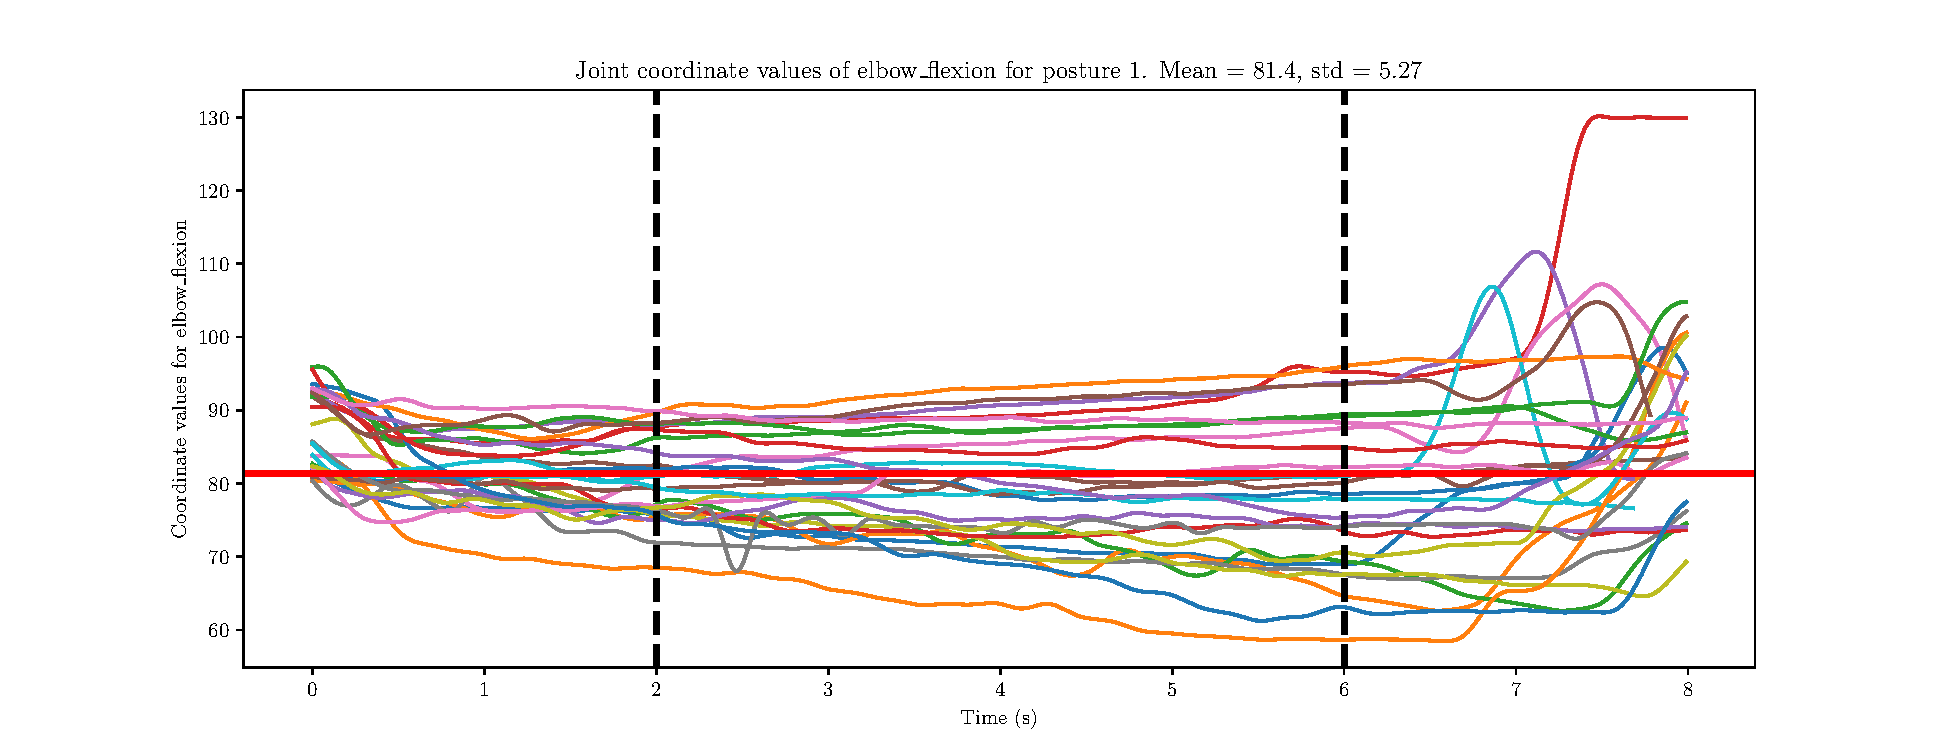
\includegraphics[trim={80 0 80 0},clip,width=1\linewidth]{img/chapter_5/posture_1_elbow_flexion_489.pdf}
    \caption{For participant 1, this graph shows their elbow flexion angle (in degrees) during all 27 force measurements in posture 1. The zone between the black dotted lines represents the timeframe where the participant exerted their maximal isometric force. The red horizontal line corresponds to the average angle value ($81.40\pm 5.27$) of all trials' mean angle values.}
    \label{fig:example_pos_489_elbow_flexion}
\end{figure}

However, since there are multiple trials to consider, Table \ref{tab:posture_stability} suggests that trials with high variability in upper-limb posture do not constitute the majority.

Overall, the trunk rotations' standard deviations are relatively small (all less than 4°) compared to other deviations. This was expected, as the trunk was strapped at the abdomen and shoulders.

Except for participants S2 and S7, the highest standard deviations in postures P1 and P2 are observed for wrist flexion angles. For participant S2, this is only the case in posture P1 (their shoulder elevation standard deviation is higher). During the experiments, it was noticed that participants tended to flex their wrists to maintain a firm grip on the handle, particularly when exerting force in the vertical direction.

Analysing all measurements within each posture (Table \ref{tab:posture_stability_ranges}) reveals that elbow flexion angles vary by up to 50° (for participant S2 in posture P1). This substantial range may be attributed to insufficient back support rigidity and the challenge of simultaneously maintaining the required posture while focusing on the direction and amplitude of force exertion.  
Regarding wrist flexion, which also exhibited a wide range of values (up to approximately 65° for participant S8 in posture P2), the difficulty of maintaining wrist position during vertical force exertions was a significant factor, as acknowledged by all participants. Additionally, while other directions allowed participants to use the palm and handle contact surface for pushing, all pulling forces required finger muscle engagement. This may have resulted in a less stable grip, potentially leading to wrist motion. Participants also reported occasional discomfort from the handle after extended use.  Furthermore, the handle design, while intended to accommodate a range of hand sizes, may have inadvertently contributed to variability in wrist flexion and deviation angles.

Although we will assume a single set of joint angles per posture and participant for the remainder of this chapter, Table \ref{tab:posture_stability} shows that, except for wrist flexion, all joint angles are generally within 20° of their mean value. This variability is mainly due to inter- and intra-trial variations in exertion. Inter-trial variability can also be attributed to the slight flexibility of the seat. Although it remained stable during the experiments, participants reported that they could settle into it. This slight movement could cause small shifts in shoulder position, contributing to variability in the overall upper-limb posture. These results suggest that while proprioceptive upper-limb placement using visual feedback may not be adequate for precise upper-limb positioning, it can be sufficient for approximate positioning.

This experimental protocol required participants to focus on their posture, the direction of force exertion, and the force amplitude simultaneously for repeated short periods. However, feedback from participants indicated that they did not find maintaining a specific posture particularly challenging. They generally found it more difficult to maintain both maximal force exertion and the correct force direction. This suggests that participants may have prioritized maximal force exertion over precise posture maintenance, leading to the observed variability in joint angles.



For the remainder of this chapter, we will use the average joint coordinate values from Table \ref{tab:posture_stability} to represent each participant's posture.

\section{Assessing the ellipsoidal characterization of in vivo force feasible set}
\label{sec:experimental_reconstruction}
To construct an \emph{in vivo} force feasible set at the hand for an upper-limb posture, we considered each force exertion measurement and defined the set as the convex hull of the corresponding force vectors. This \emph{in vivo} force feasible set, consequently a polytope, accounts for variations in force direction, which proved challenging for participants to maintain consistently. Figure \ref{fig:in_vivo_ffs_example_posture3} illustrates how maximal force production, reflected in polytope size, differs between two participants in posture P3.

\begin{figure}[!htb]
    \centering
    \captionsetup{justification=centering}
    
    \begin{minipage}{1\linewidth}
        \captionsetup{justification=centering}
        \centering
        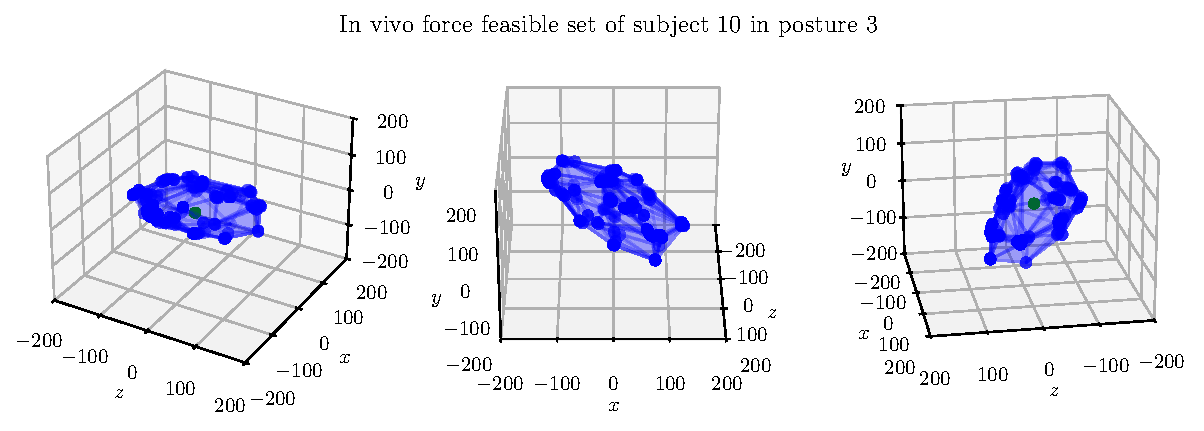
\includegraphics[trim={0 0 0 0}, clip, width=1\linewidth]{img/chapter_5/subject_21_ffs_posture_3.pdf}
    \end{minipage}

    \begin{minipage}{1\linewidth}
        \captionsetup{justification=centering}
        \centering
        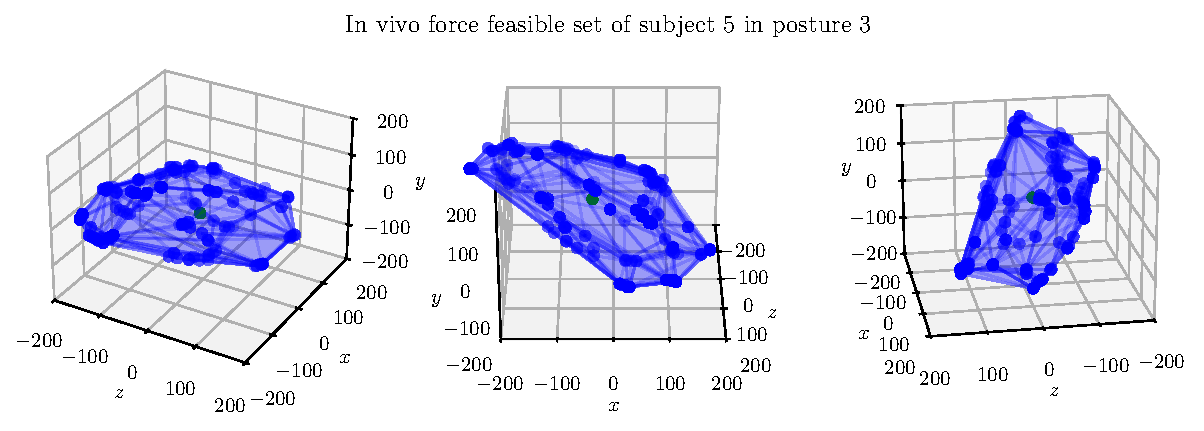
\includegraphics[trim={0 0 0 0}, clip, width=1\linewidth]{img/chapter_5/subject_296_ffs_posture_3.pdf}
    \end{minipage}
    \caption{Comparison of \emph{in vivo} force feasible sets (polytopes) for participants S10 and S5 in posture P3. Axes $x$, $y$ and $z$ are in Newtons and their direction correspond to the workspace axes ($x$-axis normal to the frontal plane; $y$-axis normal to the transverse plane and $z$-axis normal to the sagittal plane).}
    \label{fig:in_vivo_ffs_example_posture3}
\end{figure}

\subsection{Representing the underlying structure of in vivo force feasible sets}
To compare the \emph{in vivo} sets (polytopes) with the \emph{in silico} ellipsoids, we need a common representation. One approach to describe the polytopes as ellipsoids is through singular value decomposition (SVD) of the data matrix, where each column represents a maximal force exertion. SVD decomposes this matrix into three matrices: an orthonormal matrix $U$, a diagonal matrix $S$, and an orthonormal matrix $V^T$, such that the original matrix equals $USV^T$. Geometrically, this describes the measured forces as an ellipsoid formed by transforming a unit sphere: first rotating it ($V^T$), then applying anisotropic dilation (scaling along different axes) via $S$, and finally rotating again ($U$). 

However, we shall argue that a SVD approach is not relevant. It inherently averages the information between points, while we assume that unmeasured forces are geometrically linked to the measured maximal forces, not simply averaged. Therefore, we utilize an alternative ellipsoid whose definition emphasizes the importance of each measured maximal force in defining the overall set.

This ellipsoid is termed the \emph{outer Löwner-John ellipsoid} (Fig. \ref{fig:outer_lj_ellipsoid}). It is unique to a convex point set (\cite{henkLownerJohnEllipsoids2012}) and corresponds to the ellipsoid enclosing the points with minimal volume (\cite{milmanAsymptoticTheoryFinite2001}).

\begin{figure}[!htb]
    \centering
    \captionsetup{justification=centering}

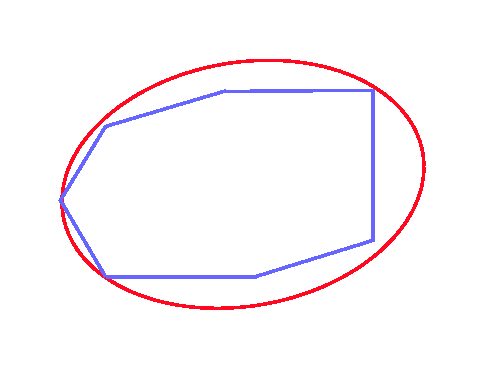
\includegraphics[trim={20 20 20 20}, clip, width=0.3\linewidth]{img/chapter_5/lowner_john_outer.pdf}
    \caption{The red ellipsoid is the outer Löwner-John ellipsoid of the blue polygon. It corresponds to the ellipsoid enclosing the points with minimal volume, and is unique to the polygon.}
    \label{fig:outer_lj_ellipsoid}
\end{figure}

While outer ellipsoids can characterize a set and reflect its structural properties due to their uniqueness, they are not necessarily used solely for approximations. However, the outer Löwner-John ellipsoid can effectively approximate sets that already exhibit an ellipsoidal shape. As discussed in Chapter \ref{chapter:3}, force feasible sets in a human upper-limb might have an ellipsoidal shape due to a high number of muscles, assuming convexity of the muscle feasible tension set. Therefore, using the outer ellipsoid to approximate the measured force exertion data could be appropriate if the data suggests an ellipsoidal shape. However, this approximation is not suitable for the data gathered in this experiment. It has not been determined whether the 26 chosen force directions adequately capture the complete \emph{in vivo} force feasible sets. For instance, to accurately capture the elongation of these sets, the chosen directions should have included their principal axes, which were unknown in this experiment.

With our data, the outer Löwner-John ellipsoid becomes relevant because it reflects the structural properties of a set. This approach relies on the assumptions that maximal muscle tensions are mathematically structured (via a norm) and that force feasible sets are produced as a transformation of this normed structure. While this can be readily described \emph{in silico} as such using Banach space theory (\emph{c.f.}, \emph{in vivo} measurements may be much more complex. Therefore, the outer ellipsoid —through its orientation, elongation, and scaling— should reveal key structural features of the unknown \emph{in vivo} force feasible sets, for which we only have a limited number of surface points. In particular, our goal is to assess whether an ellipsoidal construction, as described in Chapter \ref{chapter:3}, aligns with the experimental data.

To compute an approximation of the outer Löwner-John ellipsoid, we describe the following optimization problem. Consider a set $\mathcal{P} = \left\{\mathbf{x}_1, \dots, \mathbf{x}_m\right\}$ of $m$ points in $\IR^n$. The outer Löwner-John ellipsoid is defined as:
$$\mathcal{E}_{\mathcal{P}} = \left\{\mathbf{x}\in \IR^n \mid \| Q\mathbf{x} - \mathbf{c} \|_2 \leq 1 \right\}$$
where $Q\in \IR^{n\times n}$ is a symmetric, positive definite matrix, $\mathbf{c}\in\IR^n$ a translation vector and $\|\cdot \|_2$ the Euclidean norm. A result from (\cite{johnExtremumProblemsWithInequalities1948}) shows that the volume of $\mathcal{E}_{\mathcal{P}}$ is proportional to $(\det{Q})^{-1/n}$. Therefore, computing the outer Löwner-John ellipsoid consists of solving the following optimization problem:
\begin{align*}
    \text{maximize } & t \\
    \text{subject to } & t\leq (\det{Q})^{1/n}, \\
    & \|Q\mathbf{x}_i - \mathbf{c}\|_2 \leq 1,\quad i=1,\dots, m, \\
    & Q \text{ is symmetric, positive definite}
\end{align*}

We provide a geometric package in Python, called \emph{hyperobjects}\footnote{\url{https://gitlab.inria.fr/auctus-team/people/gautierlaisne/public/hyperobjects}}, which implements this optimization problem.

In summary, outer Löwner-John ellipsoids are specific ellipsoids uniquely associated with a set of points. While they can be used to approximate a set, their computational cost for large datasets often limits this application. However, they hold a prominent place in theoretical mathematics due to their ability to capture the geometry of a set (\cite{johnExtremumProblemsWithInequalities1948}; \cite{dvoretzkyTHEOREMCONVEXBODIES1961}; \cite{grunbaumProjectionConstants1960}; \cite{goffinRelationshipHausdorffDistance1983}; \cite{milmanDvoretzkyTheoremThirtyYearsLater1992}; \cite{henkLownerJohnEllipsoids2012}). Much of the local theory of Banach spaces, as described in Chapter \ref{chapter:3}, is based on Löwner and John's results concerning inner (maximum volume inscribed ellipsoid) and outer ellipsoids. These results help describe how the geometry of high-dimensional convex sets transforms under intersection and projection. More generally, these ellipsoids reveal the underlying mathematical structure of a set, assuming such structure exists. Consequently, Löwner-John ellipsoids may not be relevant for sets lacking inherent structure.

One of our objectives in this chapter is to assess whether a limited number of maximal isometric force measurements, which correspond to points on the surface of \emph{in vivo} force feasible sets, exhibit an ellipsoidal structure. This ellipsoidal approximation, initially proposed in Chapter \ref{chapter:3} for models with many muscles, also appeared relevant for the 50-muscle model explored in Chapter \ref{chapter:4}. To ensure consistency, we now validate whether these constructed ellipsoidal approximations align with \emph{in vivo} data.

For each participant and posture, the outer Löwner-John ellipsoid encompassing all maximal isometric force exertions is computed, as illustrated in Figure \ref{fig:in_vivo_lj_ffs_example_posture1}.
\begin{figure}[!htb]
    \centering
    \captionsetup{justification=centering}
    
    \begin{minipage}{1\linewidth}
        \captionsetup{justification=centering}
        \centering
        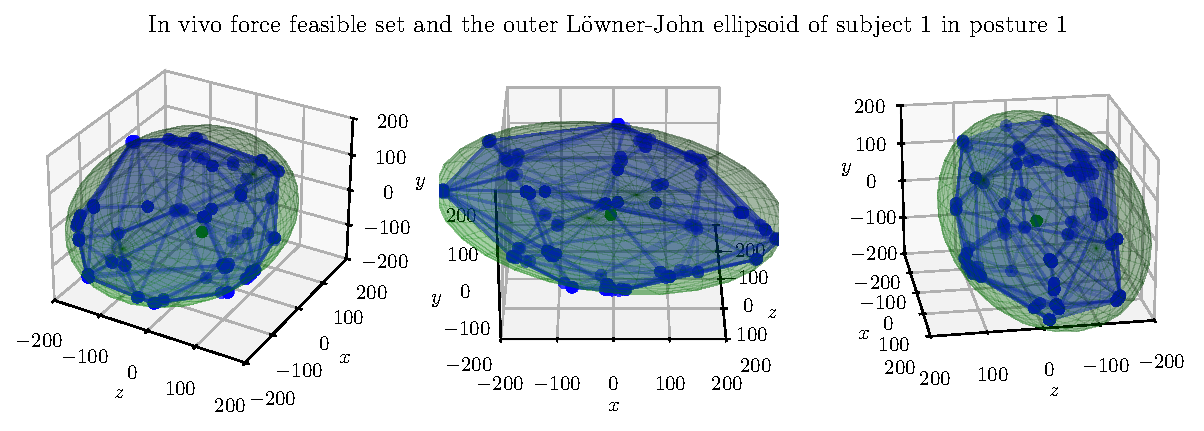
\includegraphics[trim={0 0 0 0}, clip, width=1\linewidth]{img/chapter_5/subject_489_lj_ffs_posture_1.pdf}
    \end{minipage}

    \begin{minipage}{1\linewidth}
        \captionsetup{justification=centering}
        \centering
        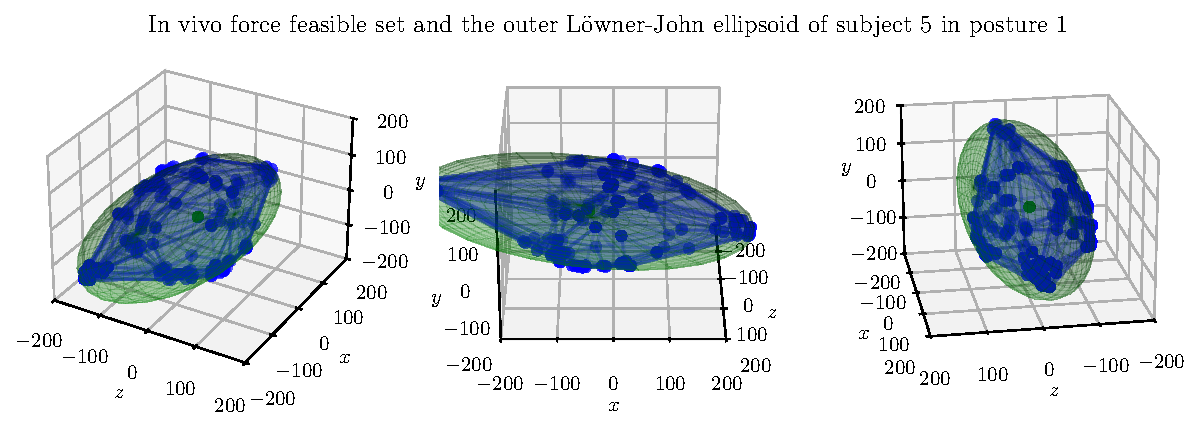
\includegraphics[trim={0 0 0 0}, clip, width=1\linewidth]{img/chapter_5/subject_296_lj_ffs_posture_1.pdf}
    \end{minipage}

    \begin{minipage}{1\linewidth}
        \captionsetup{justification=centering}
        \centering
        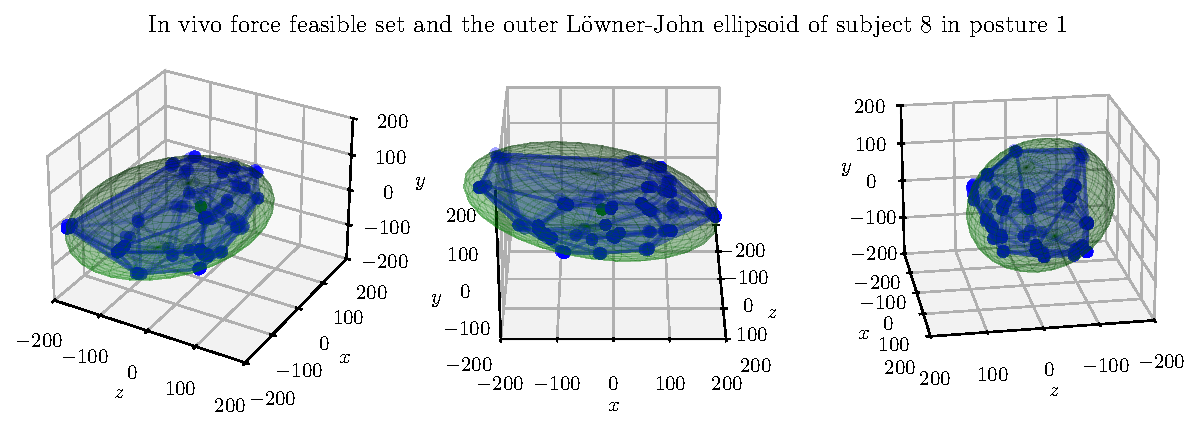
\includegraphics[trim={0 0 0 0}, clip, width=1\linewidth]{img/chapter_5/subject_163_lj_ffs_posture_1.pdf}
    \end{minipage}
    \caption{Computation of the outer Löwner-John ellipsoid (in green) from the convex hull of all maximal force measurements (blue polytope) for participants S1, S5 and S8 in posture P1.}
    \label{fig:in_vivo_lj_ffs_example_posture1}
\end{figure}

\clearpage
\subsection{Quantifying the relevance of in silico ellipsoidal force feasible sets}
The upper-limb musculoskeletal model from (\cite{holzbaurModelUpperExtremity2005}) was scaled to each participant, using OpenSim software and its integrated scaling tools. Each muscle path points coordinates description in their respective body of definition was kept untouched during this scaling. The personalization of each muscle force-generating parameters was not effected due to the Chapter \ref{chapter:3} theoretical results, which induced a strong biomechanical assumption explained in the following paragraphs.

The ellipsoidal approximation of force feasible sets results from an approximation of the muscle feasible tension set, as long as it is convex, as an ellipsoid. The projection-then-intersection of this tension ellipsoid leads consequently to force feasible sets shaped as ellipsoids. When the feasible tension set $\mathcal{T}$ is assumed to be an orthotope (hyperrectangle), assuming that it can be regarded as an ellipsoid (scaled by a factor termed the \emph{projection constant}) implies that the sharpness of $\mathcal{T}$ can be regarded as a quadratic surface (an ellipsoid) when studying the produced force feasible set. If the edges of $\mathcal{T}$ are all of the same length, then $\mathcal{T}$ is a hypercube and therefore its shape can be regarded as a sphere. Essentially, when $\mathcal{T}$ is a cube, then considering that force feasible sets are ellipsoids consists on assuming that the sharpness induced by a cube shape can be \emph{averaged} to a spherical surface. Consequently, the Local Theory of Banach spaces provides a mathematical toolkit to generalize the notion of \emph{average}, commonly used for scalars (through the notion of mean) and for points (through the notion of barycenter). To some extent, this theory generalizes this notion to convex surfaces.

If the lengths of $\mathcal{T}$'s edges are considered to be within a similar range of values, we can approximate it with the hypercube $[\underline{t},\, \overline{t}]^m$, where $m$ is the number of muscles considered, $\underline{t}$ is the mean of minimal muscle tensions, and $\overline{t}$ is the mean of maximal muscle tensions. This representation treats the muscle feasible tension set as a sphere of radius $\frac{\overline{t} - \underline{t}}{2}$ centered at $\left(\frac{\overline{t} - \underline{t}}{2} + \underline{t}\right)\mathbf{1}^m$, where $\mathbf{1}^m=(1,\dots, 1)\in \IR^m$. To ensure consistency with the cubical representation, this sphere is then scaled by the projection factor $\lambda(\ell_2^n)$ defined in Chapter \ref{chapter:3}. This scaling ensures that the resulting ellipsoidal force feasible set has a similar scale to the polytopic force feasible set.

Biomechanically, these assumptions imply that the individual minimal and maximal tension values of each muscle do not strongly influence the resulting force feasible set. Instead, as emphasized throughout this thesis, the combination of these tensions, regardless of the specific interaction model, primarily determines the force feasible set's characteristics. Essentially, only an average maximal tension value is necessary for approximating force feasible sets, eliminating the need for personalized force-generating muscle properties. This raises a critical question: \emph{under what conditions can maximal tension values be considered similar?} For example, if the maximal tensions of $m$ muscles range from 500 to 1200 Newtons, averaging these values might initially seem inappropriate. However, the consideration of muscle tension interactions, particularly as $m$ increases greatly, significantly mitigates this concern.  Since the volume of any sphere in $\IR^m$ with a fixed radius approaches 0 as $m$ tends to $\infty$, there exists a threshold for the number of muscles beyond which averaging values between 500 and 1200 becomes reasonable.

Therefore, if the number of muscles is sufficiently large, our projection-then-intersection description suggests that the global scales and shapes of force feasible sets are primarily determined by: 1) mean minimal ($\underline{t}$) and maximal ($\overline{t}$) tensions (which depend on the posture), 2) a projection constant $\lambda(\ell_p^m)$ for a chosen $p$ representing the degree of tension interactions, and 3) the Jacobian transpose $J^T$. While it may be interesting, we do not consider that all muscle tensions should be averaged, even in strong theoretical assumption of a high number of muscles. Besides, a large variability between peak forces in upper-limb muscles has been observed, for instance as recalled in (\cite{holzbaurModelUpperExtremity2005}), peak forces ranges from 13.1 (for the extensor digitorum communis of the fifth digit) to 1377.8 Newtons (for the subscapularis muscle). However, in order to use an ellipsoidal representation to its full extent, we shall assume that there are less variability of peak force for a given muscle in different postures. 

To investigate this assumption, we performed an optimization process 10 times for each participant to find a parametrization of their scaled upper-limb musculoskeletal model (based on (\cite{holzbaurModelUpperExtremity2005})). The \emph{in vivo} force feasible sets are represented as centered outer Löwner-John ellipsoids in selected postures, denoted $\hat{\mathcal{E}}(\mathbf{q})$, where $\mathbf{q}$ represents a posture as described in Section \ref{sec:posture_stability}. These ellipsoids are centered at the origin to focus on evaluating the similarity between \emph{in silico} and \emph{in vivo} force ellipsoids with respect to their orientation and elongation. The parameter vector of a solution consists of 50 values $\overline{\mathbf{t}} = (\overline{t_1}, \dots, \overline{t_{50}})$, representing the average maximal tension for each muscle in the scaled musculoskeletal model.

The force ellipsoids produced by a solution $\overline{\mathbf{t}}$ are denoted $\mathcal{E}(\mathbf{q}, \overline{\mathbf{t}})$ and are constructed as follows:
\begin{align*}
    \mathcal{E}(\mathbf{q}, \overline{\mathbf{t}}) &= \left\{ \mathbf{f} \in \IR^3 \mid J^T(\mathbf{q})\mathbf{f} = -L^T(\mathbf{q})\mathbf{t}, \quad \mathbf{t}\in [\mathbf{0}, \lambda(\ell_2^{50})\overline{\mathbf{t}}] \text{ and } \|\mathbf{t}\|_2 \leq 1\right\},
\end{align*}
where $\lambda(\ell_2^{50}) \approx 5.67$ is the projection constant that scales the resulting force feasible set to appropriately account for muscle tension interactions modeled as an ellipsoid; $J^T(\mathbf{q})\in\IR^{7\times 3}$ is the transpose of the Jacobian matrix evaluated at the hand point $X = [0.0028, -0.0339, -0.0051]$ (in meters), which approximates the center of the palm in contact with the handle; and $-L^T(\mathbf{q})\in\IR^{7\times 50}$ is the transpose of the moment arm matrix at posture $\mathbf{q}$.

Geometrically, this corresponds to first considering an axis-aligned 50-dimensional ellipsoid inscribed in the hyperrectangle $[0, \overline{t_1}]\times \dots \times [0,\lambda(\ell_2^{50})\overline{t_{50}}]$, then projecting it onto the torque space and intersecting it with $\im{J^T(\mathbf{q})}$. Finally, this intersection set is expressed in the Cartesian force space by applying $(J^T(\mathbf{q}))^+$ to it.

The optimization problem is thus formulated as:
\begin{align*}
    \theta^* = \argmin_{\theta \in [0, 1500]^{50}} \max_{\mathbf{q}\in\mathcal{Q}} d(\hat{\mathcal{E}}(\mathbf{q}),\, \mathcal{E}(\mathbf{q}, \theta)),
\end{align*}
where $\mathcal{Q} = \{P1, \, P2,\, P3\}$ is the set of the first three postures, and $d$ is the Hausdorff distance between the discretized representations (using 6 points) of the two ellipsoids.

This optimization process searches for suitable muscle maximal tensions that reproduce the \emph{in vivo} force feasible sets in the three postures. The fourth posture, P4, will be used to validate the generalizability of the solution.

\subsection{Results}
\label{subsec:results_chapt5}
The optimization process was run 10 times per participant using the RACOS solver, for a duration of 1 minute per trial. The optimization processes were implemented in Python 3 using our custom geometric package \emph{hyperobjects}\footnote{\url{https://gitlab.inria.fr/auctus-team/people/gautierlaisne/public/hyperobjects}} and the \emph{Zoopt} library for the implementation of RACOS\footnote{\url{https://zoopt.readthedocs.io/en/latest/}}. All experimental data and computed solutions are available online\footnote{\url{https://gitlab.inria.fr/auctus-team/people/gautierlaisne/public/force-experimentation-data}}.

For each solution and posture, the orientation of the \emph{in silico} force ellipsoid relative to the \emph{in vivo} outer Löwner-John ellipsoid is studied by comparing the relative angles between their principal axes. These axes are denoted D1, D2, and D3, in decreasing order of the corresponding singular values obtained through singular value decomposition of the matrix describing the ellipsoid as a linear transformation of the sphere. Thus, D1 is associated with the axis of greatest elongation, and D3 with the axis of least elongation. For two axes, $D\in\IR^3$ and $\hat{D}\in\IR^3$ (one for each ellipsoid), the relative angle (in degrees) is computed as $\alpha_D = \arccos\left(\frac{D \cdot \hat{D}}{\|D\|\|\hat{D}\|}\right)$ and is expressed in the range $[0^\circ, 90^\circ]$.

To compare the elongation differences between two ellipsoids, we collect the semi-axis lengths (termed "radii") and compute their absolute differences. Table \ref{tab:angle_between_direction} presents these comparison indices after the 10 optimization runs.

\begin{table}[!ht]
    \centering
    \captionsetup{justification=centering}
    \resizebox{\textwidth}{!}{
    \begin{tabular}{|c|c|c||c|c|c||c|c|c|}
    \hline
    \textbf{Subject} & \makecell{\textbf{Posture}} & \makecell{\textbf{Cost}} & \makecell{\textbf{Angle} \\ \textbf{D1}} & \makecell{\textbf{Angle} \\ \textbf{D2}} & \makecell{\textbf{Angle} \\ \textbf{D3}} & \makecell{\textbf{Absolute radius} \\ \textbf{difference D1}} & \makecell{\textbf{Absolute radius} \\ \textbf{difference D2}} & \makecell{\textbf{Absolute radius} \\ \textbf{difference D3}} \\
    \hline
    \multirow{3}{*}{S1} & P1 & $49\pm 21$ & $11\pm 5$ & $58\pm 25$ & $58\pm 25$ & $85\pm 36$ & $31\pm 17$ & $52\pm 22$ \\
    & P2 & $37\pm 16$ & $8\pm 4$ & $68\pm 29$ & $67\pm 29$ & $82\pm 35$ & $35\pm 16$ & $26\pm 15$ \\
    & P3 & $48\pm 20$ & $8\pm 4$ & $12\pm 13$ & $14\pm 13$ & $74\pm 38$ & $16\pm 12$ & $40\pm 17$ \\
    % & P4 & $117\pm 52$ & $16\pm 7$ & $67\pm 30$ & $66\pm 30$ & $38\pm 20$ & $23\pm 18$ & $55\pm 24$ \\
    \hline
    \hline
    \multirow{3}{*}{S2} & P1 & $123\pm 29$ & $21\pm 2$ & $61\pm 4$ & $58\pm 4$ & $86\pm 59$ & $23\pm 19$ & $34\pm 18$ \\
    & P2 & $109\pm 18$ & $11\pm 2$ & $55\pm 6$ & $56\pm 5$ & $69\pm 37$ & $22\pm 14$ & $32\pm 19$ \\
    & P3 & $121\pm 29$ & $18\pm 1$ & $21\pm 4$ & $17\pm 4$ & $66\pm 36$ & $18\pm 10$ & $31\pm 15$ \\
    % & P4 & $88\pm 25$ & $8\pm 3$ & $60\pm 13$ & $60\pm 13$ & $81\pm 29$ & $18\pm 11$ & $26\pm 18$ \\
    \hline
    \hline
    \multirow{3}{*}{S3} & P1 & $90\pm 34$ & $16\pm 2$ & $42\pm 9$ & $44\pm 9$ & $73\pm 43$ & $36\pm 24$ & $30\pm 18$ \\
    & P2 & $63\pm 23$ & $13\pm 4$ & $52\pm 30$ & $54\pm 30$ & $97\pm 60$ & $25\pm 16$ & $22\pm 15$ \\
    & P3 & $90\pm 34$ & $10\pm 1$ & $33\pm 14$ & $32\pm 14$ & $189\pm 109$ & $38\pm 30$ & $20\pm 11$ \\
    % & P4 & $202\pm 74$ & $14\pm 2$ & $82\pm 4$ & $81\pm 5$ & $168\pm 114$ & $36\pm 29$ & $25\pm 13$ \\
    \hline
    \hline
    \multirow{3}{*}{S4} & P1 & $99\pm 25$ & $18\pm 4$ & $44\pm 32$ & $48\pm 27$ & $92\pm 59$ & $66\pm 29$ & $56\pm 30$ \\
    & P2 & $95\pm 19$ & $8\pm 2$ & $47\pm 11$ & $47\pm 11$ & $113\pm 75$ & $67\pm 26$ & $80\pm 29$ \\
    & P3 & $104\pm 21$ & $10\pm 1$ & $29\pm 8$ & $30\pm 8$ & $126\pm 75$ & $44\pm 30$ & $67\pm 25$ \\
    % & P4 & $42\pm 26$ & $3\pm 2$ & $77\pm 10$ & $77\pm 10$ & $76\pm 60$ & $74\pm 23$ & $67\pm 25$ \\
    \hline
    \hline
    \multirow{3}{*}{S5} & P1 & $96\pm 32$ & $12\pm 3$ & $54\pm 14$ & $55\pm 14$ & $72\pm 58$ & $57\pm 45$ & $24\pm 16$ \\
    & P2 & $81\pm 23$ & $10\pm 2$ & $19\pm 11$ & $20\pm 11$ & $57\pm 47$ & $44\pm 36$ & $29\pm 14$ \\
    & P3 & $96\pm 32$ & $14\pm 2$ & $59\pm 25$ & $60\pm 24$ & $69\pm 62$ & $40\pm 35$ & $23\pm 24$ \\
    % & P4 & $91\pm 45$ & $12\pm 5$ & $80\pm 6$ & $80\pm 6$ & $117\pm 90$ & $38\pm 34$ & $20\pm 19$ \\
    \hline
    \hline
    \multirow{3}{*}{S6} & P1 & $124\pm 30$ & $15\pm 2$ & $13\pm 6$ & $20\pm 4$ & $68\pm 59$ & $97\pm 47$ & $22\pm 16$ \\
    & P2 & $75\pm 27$ & $9\pm 2$ & $19\pm 17$ & $21\pm 16$ & $66\pm 62$ & $62\pm 41$ & $22\pm 19$ \\
    & P3 & $124\pm 30$ & $14\pm 2$ & $27\pm 17$ & $31\pm 16$ & $69\pm 36$ & $46\pm 34$ & $25\pm 19$ \\
    % & P4 & $109\pm 21$ & $11\pm 3$ & $53\pm 10$ & $54\pm 11$ & $83\pm 74$ & $68\pm 34$ & $24\pm 25$ \\
    \hline
    \hline
    \multirow{3}{*}{S7} & P1 & $98\pm 39$ & $16\pm 2$ & $49\pm 11$ & $50\pm 10$ & $95\pm 63$ & $48\pm 30$ & $50\pm 37$ \\
    & P2 & $69\pm 32$ & $6\pm 3$ & $28\pm 8$ & $28\pm 8$ & $137\pm 94$ & $47\pm 32$ & $42\pm 32$ \\
    & P3 & $100\pm 39$ & $15\pm 2$ & $39\pm 6$ & $37\pm 6$ & $87\pm 74$ & $49\pm 37$ & $43\pm 31$ \\
    % & P4 & $108\pm 32$ & $15\pm 5$ & $37\pm 9$ & $37\pm 9$ & $79\pm 61$ & $39\pm 31$ & $60\pm 23$ \\
    \hline
    \hline
    \multirow{3}{*}{S8} & P1 & $79\pm 39$ & $13\pm 6$ & $84\pm 4$ & $85\pm 4$ & $88\pm 59$ & $81\pm 52$ & $13\pm 10$ \\
    & P2 & $90\pm 24$ & $17\pm 4$ & $23\pm 14$ & $15\pm 16$ & $38\pm 31$ & $39\pm 22$ & $39\pm 24$ \\
    & P3 & $91\pm 24$ & $14\pm 2$ & $63\pm 13$ & $64\pm 13$ & $86\pm 61$ & $85\pm 26$ & $24\pm 18$ \\
    % & P4 & $96\pm 22$ & $13\pm 3$ & $48\pm 17$ & $46\pm 19$ & $73\pm 57$ & $15\pm 10$ & $18\pm 7$ \\
    \hline
    \hline
    \multirow{3}{*}{S9} & P1 & $44\pm 26$ & $6\pm 3$ & $74\pm 16$ & $74\pm 16$ & $77\pm 79$ & $35\pm 30$ & $42\pm 27$ \\
    & P2 & $43\pm 25$ & $6\pm 3$ & $80\pm 14$ & $80\pm 14$ & $77\pm 51$ & $31\pm 19$ & $48\pm 24$ \\
    & P3 & $41\pm 19$ & $6\pm 3$ & $72\pm 14$ & $72\pm 14$ & $73\pm 48$ & $28\pm 20$ & $48\pm 28$ \\
    % & P4 & $80\pm 23$ & $7\pm 4$ & $47\pm 20$ & $47\pm 20$ & $126\pm 79$ & $23\pm 21$ & $32\pm 25$ \\
    \hline
    \hline
    \multirow{3}{*}{S10} & P1 & $68\pm 20$ & $10\pm 4$ & $66\pm 4$ & $65\pm 5$ & $59\pm 53$ & $41\pm 26$ & $17\pm 10$ \\
    & P2 & $66\pm 20$ & $12\pm 2$ & $45\pm 21$ & $43\pm 23$ & $122\pm 65$ & $29\pm 22$ & $22\pm 18$ \\
    & P3 & $65\pm 19$ & $10\pm 2$ & $23\pm 6$ & $23\pm 6$ & $175\pm 61$ & $51\pm 29$ & $38\pm 20$ \\
    % & P4 & $88\pm 23$ & $7\pm 3$ & $49\pm 6$ & $49\pm 7$ & $153\pm 90$ & $48\pm 26$ & $15\pm 13$ \\
    \hline
    \end{tabular}}
    \caption{Comparison of the produced ellipsoids and the \emph{in vivo} outer Löwner-John ellipsoids for each participant across 10 optimization trials.  The table presents the mean and standard deviation (rounded to the nearest integer) of: (1) the angle (in degrees, within $[0^\circ, 90^\circ]$) between corresponding principal axes (D1, D2, D3, sorted in decreasing order of axis length), and (2) the absolute difference in semi-axis length (in Newtons) for each principal axis.}
    \label{tab:angle_between_direction}
\end{table}

\subsubsection*{Validation posture}
Similarly to Table \ref{tab:angle_between_direction}, Table \ref{tab:angle_between_direction_validation} presents the orientation and elongation differences between the reconstructed ellipsoid from maximal isometric force measurements in posture P4 and the force ellipsoid constructed by the solutions found in the optimization processes.

\begin{table}[!ht]
    \centering
    \captionsetup{justification=centering}
    \resizebox{\textwidth}{!}{
    \begin{tabular}{|c|c|c||c|c|c||c|c|c|}
    \hline
    \textbf{Subject} & \makecell{\textbf{Posture}} & \makecell{\textbf{Cost}} & \makecell{\textbf{Angle} \\ \textbf{D1}} & \makecell{\textbf{Angle} \\ \textbf{D2}} & \makecell{\textbf{Angle} \\ \textbf{D3}} & \makecell{\textbf{Absolute radius} \\ \textbf{difference D1}} & \makecell{\textbf{Absolute radius} \\ \textbf{difference D2}} & \makecell{\textbf{Absolute radius} \\ \textbf{difference D3}} \\
    \hline
    S1 & P4 & $117\pm 52$ & $16\pm 7$ & $67\pm 30$ & $66\pm 30$ & $38\pm 20$ & $23\pm 18$ & $55\pm 24$ \\
    \hline
    S2 & P4 & $88\pm 25$ & $8\pm 3$ & $60\pm 13$ & $60\pm 13$ & $81\pm 29$ & $18\pm 11$ & $26\pm 18$ \\
    \hline
    S3 & P4 & $202\pm 74$ & $14\pm 2$ & $82\pm 4$ & $81\pm 5$ & $168\pm 114$ & $36\pm 29$ & $25\pm 13$ \\
    \hline
    S4 & P4 & $42\pm 26$ & $3\pm 2$ & $77\pm 10$ & $77\pm 10$ & $76\pm 60$ & $74\pm 23$ & $67\pm 25$ \\
    \hline
    S5 & P4 & $91\pm 45$ & $12\pm 5$ & $80\pm 6$ & $80\pm 6$ & $117\pm 90$ & $38\pm 34$ & $20\pm 19$ \\
    \hline
    S6 & P4 & $109\pm 21$ & $11\pm 3$ & $53\pm 10$ & $54\pm 11$ & $83\pm 74$ & $68\pm 34$ & $24\pm 25$ \\
    \hline
    S7 & P4 & $108\pm 32$ & $15\pm 5$ & $37\pm 9$ & $37\pm 9$ & $79\pm 61$ & $39\pm 31$ & $60\pm 23$ \\
    \hline
    S8 & P4 & $96\pm 22$ & $13\pm 3$ & $48\pm 17$ & $46\pm 19$ & $73\pm 57$ & $15\pm 10$ & $18\pm 7$ \\
    \hline
    S9 & P4 & $80\pm 23$ & $7\pm 4$ & $47\pm 20$ & $47\pm 20$ & $126\pm 79$ & $23\pm 21$ & $32\pm 25$ \\
    \hline
    S10 & P4 & $88\pm 23$ & $7\pm 3$ & $49\pm 6$ & $49\pm 7$ & $153\pm 90$ & $48\pm 26$ & $15\pm 13$ \\
    \hline
    \end{tabular}}
    \caption{Similar as Table \ref{tab:angle_between_direction} but for validation posture P4.}
    \label{tab:angle_between_direction_validation}
\end{table}

\clearpage
\subsection*{Qualitative assessment of reproduced force feasible sets}
To qualitatively assess the differences between the 3D shapes, Figures \ref{fig:sub8_7thsol}, \ref{fig:sub6_4thsol}, and \ref{fig:sub9_7thsol} show the ellipsoid produced by one of the 10 solutions (in red) superimposed on the outer Löwner-John ellipsoids (in green) computed from the measurements (blue polytope).

\begin{figure}[!htb]
    \centering
    \captionsetup{justification=centering}
    \begin{minipage}{1\linewidth}
        \captionsetup{justification=centering}
        \centering
        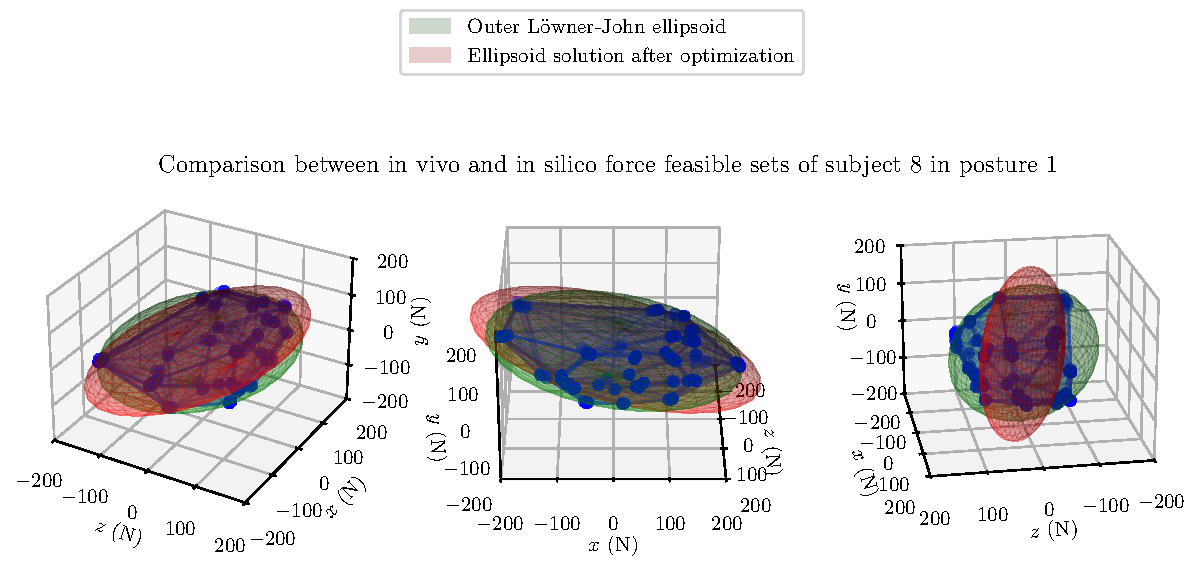
\includegraphics[trim=0 0 0 60, clip, width=0.8\linewidth]{img/chapter_5/subject_163_solution_7_posture_1.pdf}
    \end{minipage}
    \hfill
    \begin{minipage}{1\linewidth}
        \captionsetup{justification=centering}
        \centering
        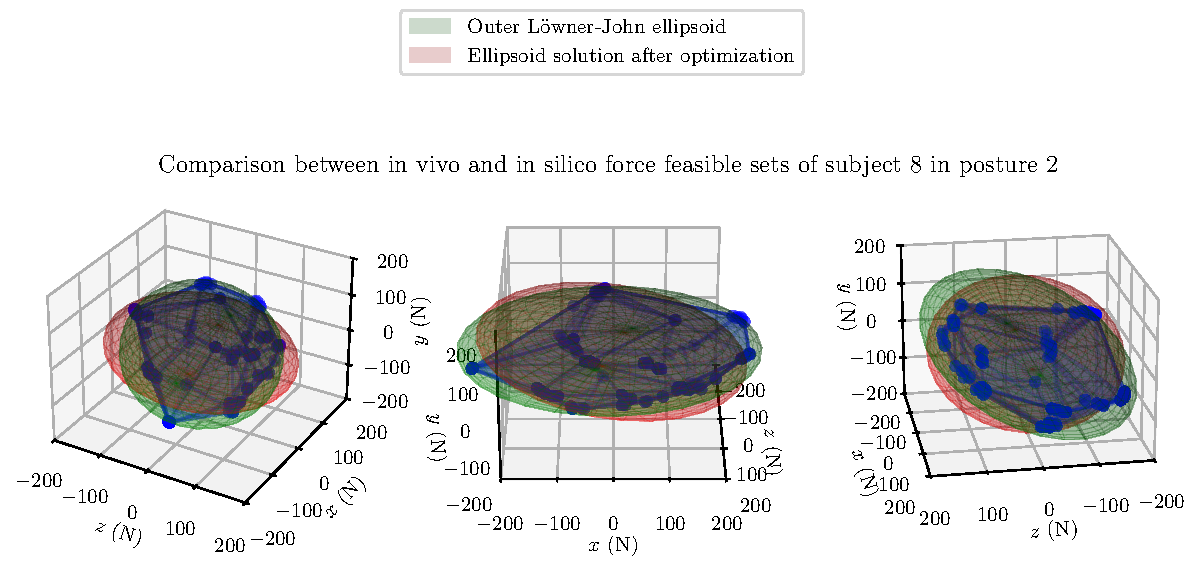
\includegraphics[trim=0 0 0 60, clip, width=0.8\linewidth]{img/chapter_5/subject_163_solution_7_posture_2.pdf}
    \end{minipage}
    \begin{minipage}{1\linewidth}
        \captionsetup{justification=centering}
        \centering
        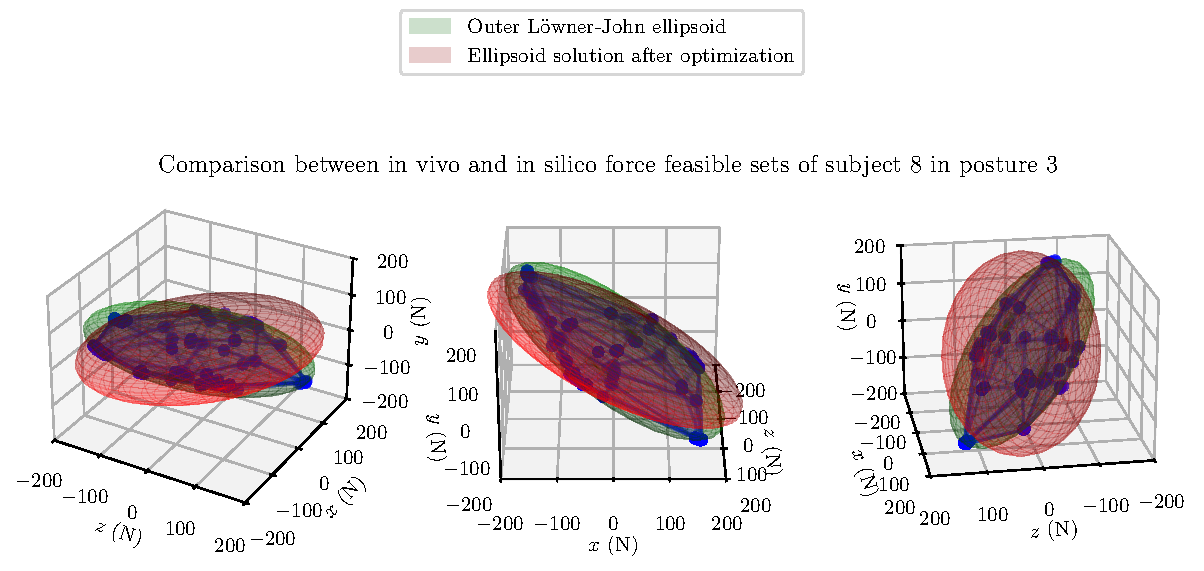
\includegraphics[trim=0 0 0 60, clip, width=0.8\linewidth]{img/chapter_5/subject_163_solution_7_posture_3.pdf}
    \end{minipage}
    \begin{minipage}{1\linewidth}
        \captionsetup{justification=centering}
        \centering
        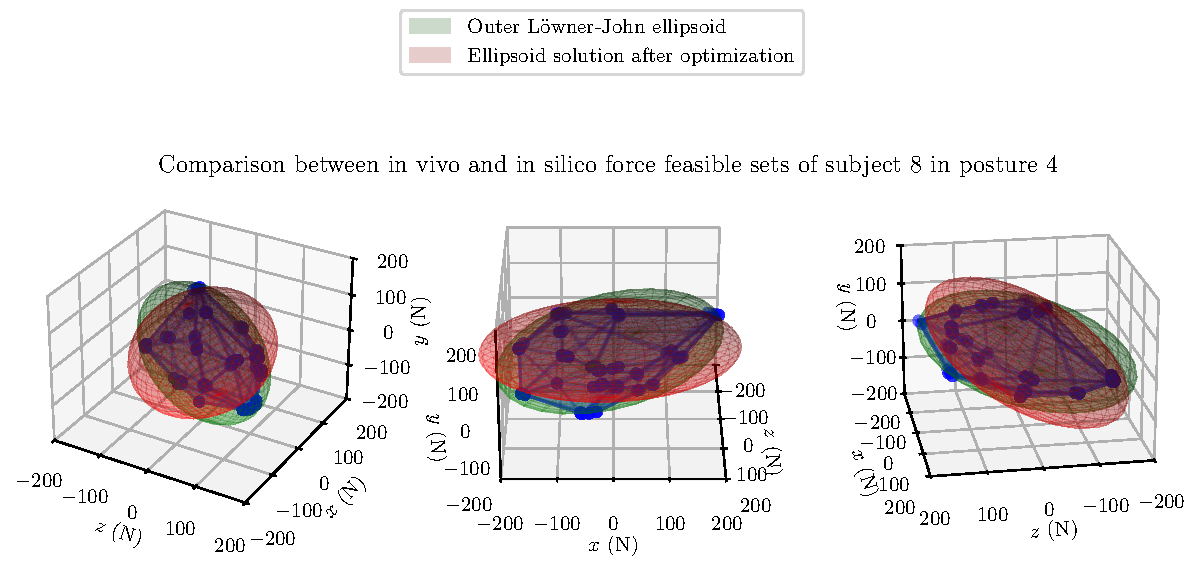
\includegraphics[trim=0 0 0 60, clip, width=0.8\linewidth]{img/chapter_5/subject_163_solution_7_posture_4.pdf}
    \end{minipage}
    \caption{Force feasible sets for participant S8 in all postures. The \emph{in vivo} force polytope is shown in blue, the associated outer Löwner-John ellipsoid in green, and the \emph{in silico} force ellipsoid computed in the 7th optimization run in red. All shapes are centered at the origin.}
    \label{fig:sub8_7thsol}
\end{figure}

\clearpage
\begin{figure}[!htb]
    \centering
    \begin{minipage}{1\linewidth}
        \captionsetup{justification=centering}
        \centering
        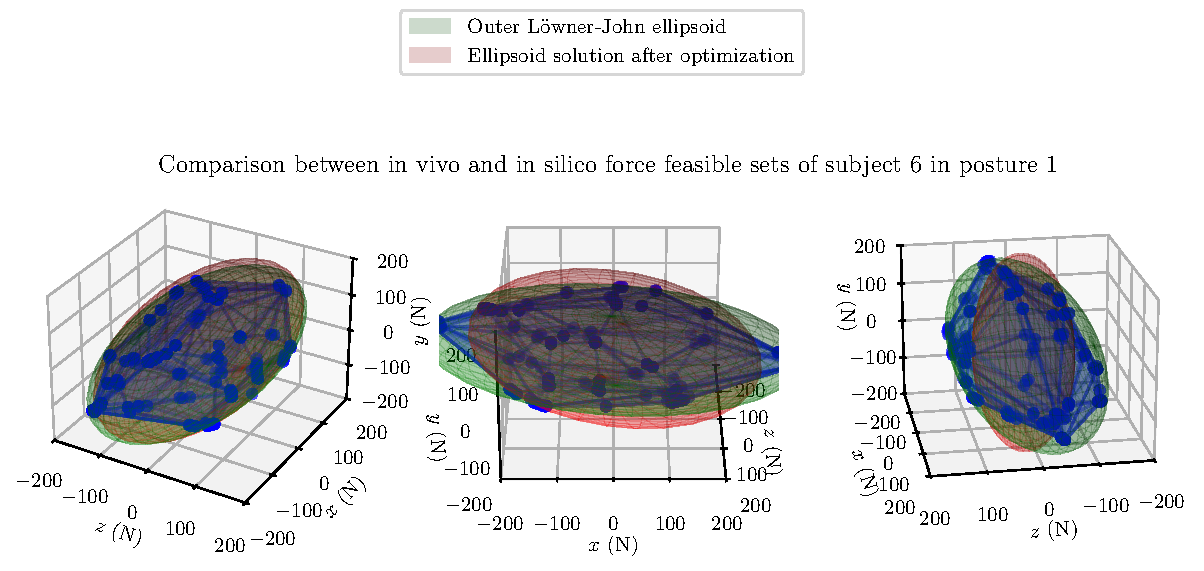
\includegraphics[trim=0 0 0 60, clip, width=0.8\linewidth]{img/chapter_5/subject_251_solution_4_posture_1.pdf}
    \end{minipage}
    \hfill
    \begin{minipage}{1\linewidth}
        \captionsetup{justification=centering}
        \centering
        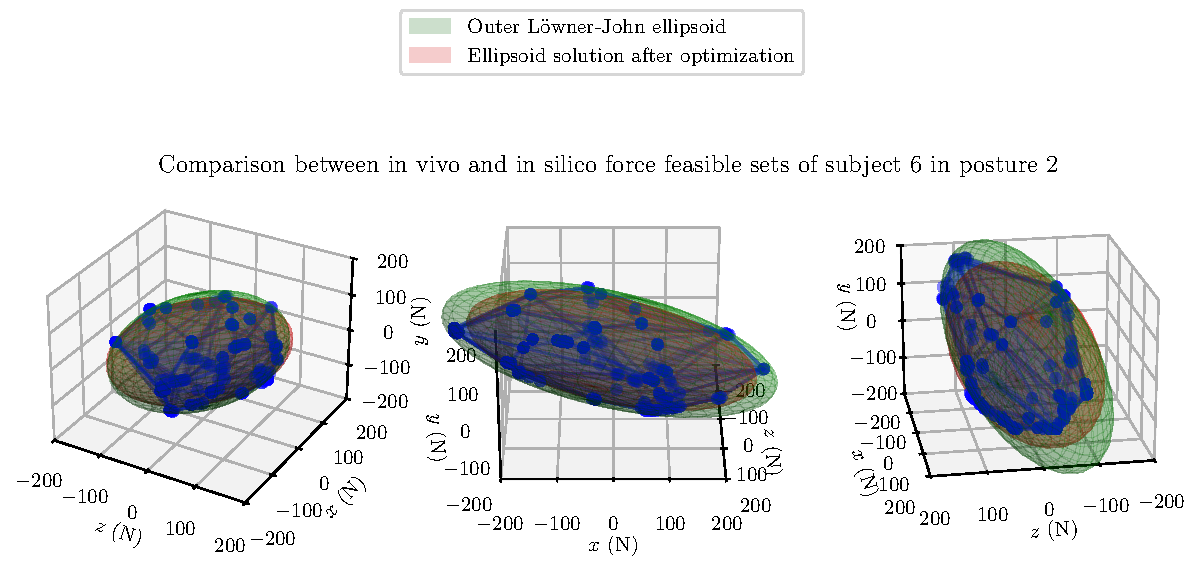
\includegraphics[trim=0 0 0 60, clip, width=0.8\linewidth]{img/chapter_5/subject_251_solution_4_posture_2.pdf}
    \end{minipage}
    \begin{minipage}{1\linewidth}
        \captionsetup{justification=centering}
        \centering
        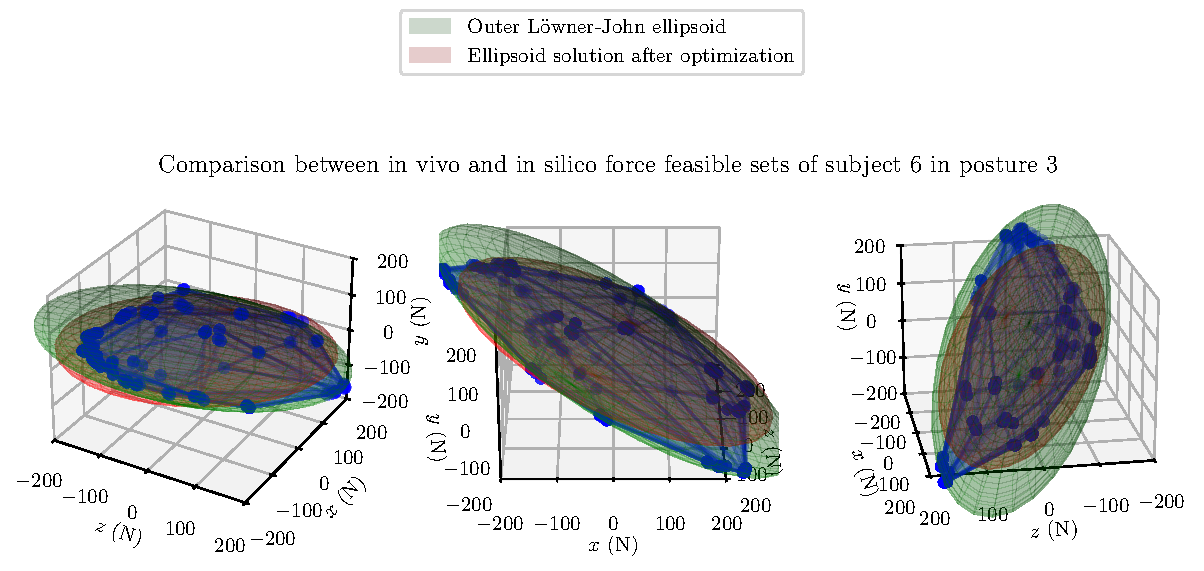
\includegraphics[trim=0 0 0 60, clip, width=0.8\linewidth]{img/chapter_5/subject_251_solution_4_posture_3.pdf}
    \end{minipage}
    \begin{minipage}{1\linewidth}
        \captionsetup{justification=centering}
        \centering
        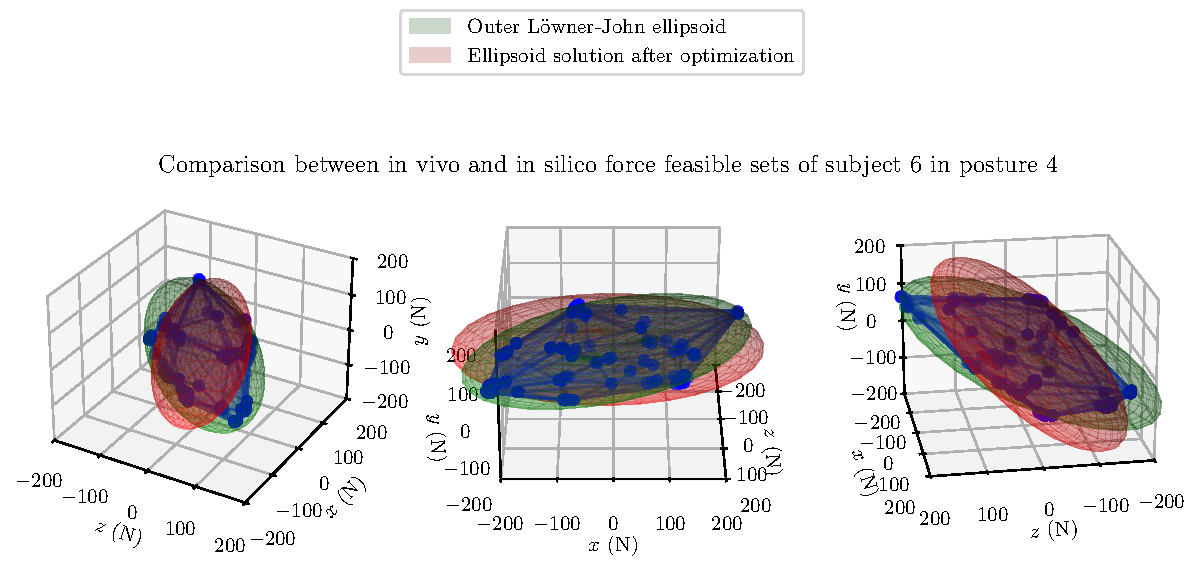
\includegraphics[trim=0 0 0 60, clip, width=0.8\linewidth]{img/chapter_5/subject_251_solution_4_posture_4.pdf}
    \end{minipage}
    \caption{Force feasible sets for participant S6 in all postures. The \emph{in vivo} force polytope is shown in blue, the associated outer Löwner-John ellipsoid in green, and the \emph{in silico} force ellipsoid computed in the 4th optimization run in red. All shapes are centered at the origin.}
    \label{fig:sub6_4thsol}
\end{figure}


\clearpage
\begin{figure}[!htb]
    \centering
    \begin{minipage}{1\linewidth}
        \captionsetup{justification=centering}
        \centering
        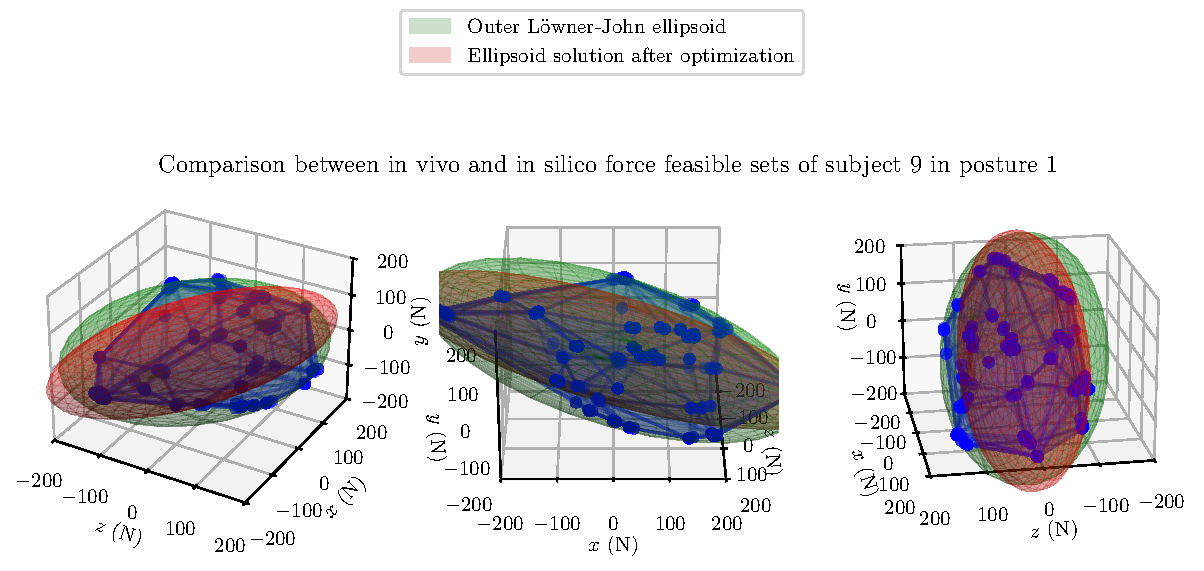
\includegraphics[trim=0 0 0 60, clip, width=0.8\linewidth]{img/chapter_5/subject_104_solution_7_posture_1.pdf}
    \end{minipage}
    \hfill
    \begin{minipage}{1\linewidth}
        \captionsetup{justification=centering}
        \centering
        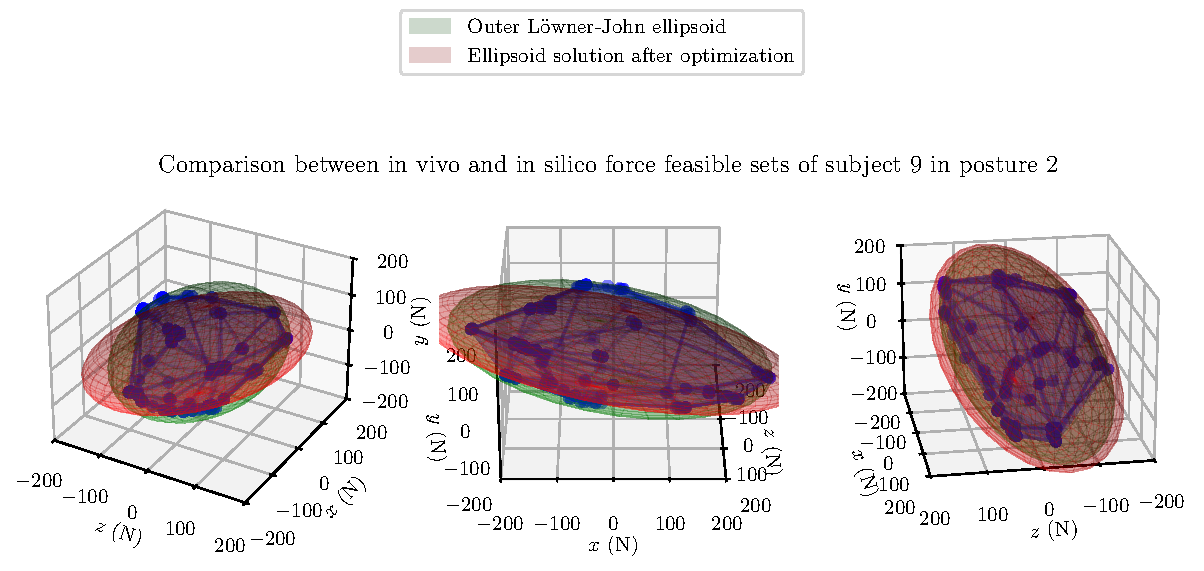
\includegraphics[trim=0 0 0 60, clip, width=0.8\linewidth]{img/chapter_5/subject_104_solution_7_posture_2.pdf}
    \end{minipage}
    \begin{minipage}{1\linewidth}
        \captionsetup{justification=centering}
        \centering
        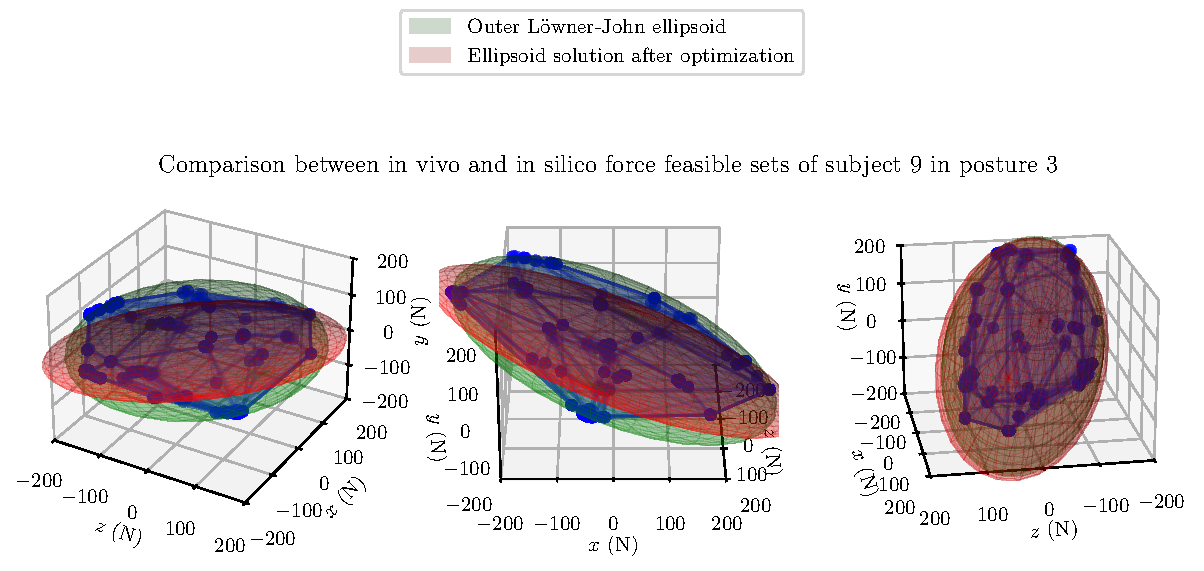
\includegraphics[trim=0 0 0 60, clip, width=0.8\linewidth]{img/chapter_5/subject_104_solution_7_posture_3.pdf}
    \end{minipage}
    \begin{minipage}{1\linewidth}
        \captionsetup{justification=centering}
        \centering
        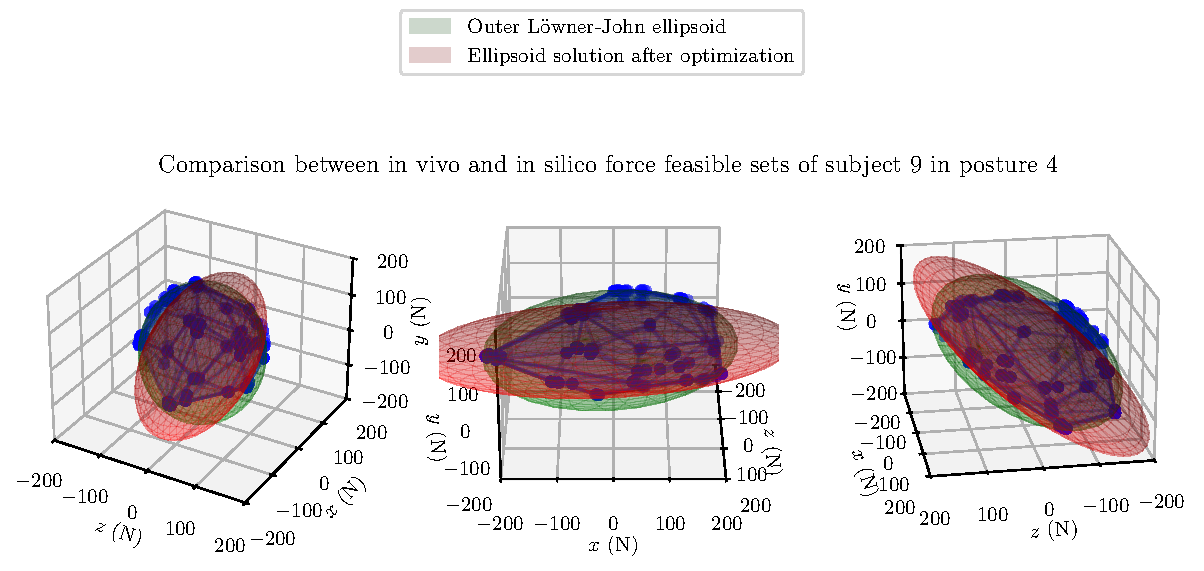
\includegraphics[trim=0 0 0 60, clip, width=0.8\linewidth]{img/chapter_5/subject_104_solution_7_posture_4.pdf}
    \end{minipage}
    \caption{Force feasible sets for participant S9 in all postures. The \emph{in vivo} force polytope is shown in blue, the associated outer Löwner-John ellipsoid in green, and the \emph{in silico} force ellipsoid computed in the 7th optimization run in red. All shapes are centered at the origin.}
    \label{fig:sub9_7thsol}
\end{figure}

\subsection{Conclusion and discussion}
The computed \emph{in silico} force ellipsoids generated by the optimization solutions were compared to the orientations and elongations of the outer Löwner-John ellipsoids derived from experimentally measured maximal isometric force exertions in 26 directions across 4 postures. The optimization process aimed to determine mean maximal tension values for 50 upper-limb muscles, under the assumption that these values do not vary significantly between postures. This assumption, while seemingly contradicting the established force-length relationship of muscles, reflects the hypothesis that muscle tension interactions have a far greater influence that the individual muscle tensions on the generation of maximal hand forces in the right upper-limb. This hypothesis is supported by the theoretical framework presented in Chapter \ref{chapter:3}, which indicates that a large number of muscles necessarily leads to this behavior when considering an ellipsoidal representation of the muscle tension feasible set. However, the required number of muscles to achieve this behavior is a theoretical value, expressed as an asymptotic function that tends to $+\infty$ as the accuracy of the ellipsoidal approximation increases. Therefore, this study aimed to evaluate the validity of this hypothesis for a musculoskeletal model with 50 muscles, as it is unclear whether this constitutes a sufficiently large number.

Furthermore, this work investigated whether representing \emph{in vivo} force feasible sets using outer Löwner-John ellipsoids, derived from measured maximal force exertions, could be more suitable than a polytopic representation. Since these ellipsoids reflect the structural information of a geometric construction process, this study compared \emph{in silico} force ellipsoids (constructed by projecting an ellipsoidal muscle tension feasible set onto the torque space and intersecting it with the image of the Jacobian transpose) with the corresponding outer Löwner-John ellipsoids across various postures. Similarities in characteristics, such as orientation and elongation, between these two representations would suggest that the construction of \emph{in silico} force ellipsoids and their underlying hypotheses are indeed inscribed in \emph{in vivo} force feasible sets and thus captured by their outer Löwner-John ellipsoid. In other words, while \emph{in vivo} force feasible sets may indeed exhibit an ellipsoidal shape, this does not necessarily validate the adequacy of their \emph{in silico} counterparts as described in this study.

Overall, the discretized Hausdorff distances (Cost column in Tables \ref{tab:angle_between_direction} and \ref{tab:angle_between_direction_validation}) between the computed force ellipsoids and the experimental outer Löwner-John ellipsoids exhibit similar values and variability across postures P1, P2, and P3. However, these similarities do not extend to posture P4. For participants S2 and S4, the costs associated with posture P4 are even lower than those observed in the fitting conditions (P1, P2, P3), suggesting that the solutions can predict force ellipsoids with greater accuracy than achieved through fitting. For the remaining participants, overfitting is observed. This discrepancy between underfitting and overfitting behaviors may indicate that the number of postures used for fitting is insufficient.

An analysis of the angles presented in both tables reveals that, for all participants and postures, the \emph{in silico} major axis (D1) exhibits the least variability and the lowest average angular deviation compared to the outer Löwner-John ellipsoid. This indicates that this direction is well-captured by our force ellipsoid model. However, large angular deviations are observed for D2 and D3 in both fitting and validation postures, with differences reaching almost 90° for participant S9 in posture P2. Notably, for all participants and postures, the angular errors for D2 are similar to those of D3. This similarity could be attributed to the high variability in participant postures, suggesting that such variability does not significantly impact the primary force direction only. Alternatively, since the angular errors for D2 and D3 are relatively similar, this could indicate a relationship between the orientations of the \emph{in silico} force ellipsoids and the outer ellipsoids, but with a need for adjusting the modeling choices in the computed force ellipsoids. This interpretation is supported by the observation that all participants and postures exhibit similar mean angular errors and standard deviations for D2 and D3, in both fitting and validation postures.

Regarding the elongation characteristics of both ellipsoids, a striking observation is the lack of consistent patterns across participants. This is evidenced by standard deviations often approaching the corresponding mean values, as seen, for instance, in direction D1, posture P2, for participants S5, S6, S8, and S9. This finding is crucial because the absence of a structured pattern in elongation contradicts our initial assumption that muscle maximal tension can be averaged across postures. Consequently, it appears that the variability of muscle maximal tensions does indeed influence the force feasible set when employing a projection-then-intersection formulation, where the theoretical consideration of simply using an ellipsoid representation suggested that it would not.

These results highlight two seemingly contradictory mathematical considerations. On one hand, the findings suggest that the outer Löwner-John ellipsoids share structural information with our \emph{in silico} force ellipsoid model. On the other hand, the outer ellipsoids do not capture the same structural information concerning elongation when assuming an averaged maximal muscle tension across postures.

In other words, while an ellipsoidal representation of \emph{in silico} force feasible sets may be appropriate regarding shape and orientation (suggesting that 50 muscles are sufficient for this purpose), the associated tension set modeling requires further refinement. The assumption that \emph{50 muscles is large enough} for an ellipsoid modeling, as suggested by Chapter \ref{chapter:3} in a pure theoretical point of view and Chapter \ref{chapter:4} from a numerical point of view, appears to hold only for modeling shape and primary force direction, but not for accurately capturing elongation. This could potentially be extended to encompass the overall orientation with further model refinements. If 50 muscles were indeed considered sufficiently large \emph{in general}, the range of maximal tension values within a muscle could be represented by an average value, leading to more structured results in the observed radius differences.

\section{Conclusion}
The goal of this chapter was to confront the theoretical assumptions regarding the relevance of modeling force feasible sets as ellipsoids with experimental data. Assuming that \emph{in vivo} force feasible sets are ellipsoidal, based on their \emph{in silico} definition (\emph{c.f.} Chapter \ref{chapter:1}), leads to significant implications for the overall modeling framework. Namely, it implies that the muscle tension feasible set can also be regarded as an ellipsoid. This geometric assumption can be understood as the geometric notion of \emph{averaging}, which, in this case, is valid as long as we are studying a high-dimensional convex object from a lower-dimensional perspective. In our context, this implies that, for a specific upper-limb posture, the convex muscle tension feasible set can be considered as an ellipsoid if its corresponding force feasible set exhibits an ellipsoidal shape. The primary requirement is that the number of muscles be sufficiently large. While this notion of \emph{large} is well-defined mathematically, it is less clear in practice, as we are using a musculoskeletal model of the upper-limb to describe \emph{in silico} force feasible sets that represent \emph{in vivo} sets.

Therefore, this chapter focused on assessing the extent to which an \emph{in silico} ellipsoidal representation of force feasible sets is appropriate when using a musculoskeletal model with 50 muscles. Our findings reveal a more nuanced answer than initially anticipated: while the shape and primary direction of force can be effectively captured by ellipsoids, the elongation of the \emph{in vivo} force feasible set is not solely determined by its ellipsoidal characterization.  We argue this point by contradicting the following: if the elongation of a force feasible set were solely a consequence of the ellipsoidal nature of the muscle tension feasible set $\mathcal{T}$, then $\mathcal{T}$ would essentially be an average shape of an orthotope (up to scale), a theoretical behavior that emerges in very high dimensions. However, in high-dimensional spaces, $\mathcal{T}$ would not vary significantly between different postures, as the variability in minimal and maximal muscle tension values across postures becomes less significant with increasing dimensionality. Under this assumption, the elongation of any produced force feasible set would depend solely on average muscle maximal tension values.

To test this hypothesis, we first collected maximal isometric force measurements. Ten participants volunteered to exert 26 maximal forces at the hand of their right upper-limb in various directions, across four different postures. The experiment was conducted in a minimum of two 3-hour sessions. Participants were seated with their abdominals and shoulders uncovered to minimize trunk motion. Contact forces were limited to reduce external constraints: participants' feet did not touch the ground, and no physical restraints were imposed on their upper-limb posture. The experimental setup was designed to accommodate individual anthropometric variability. Participants were simply asked to sit and position their hand on a handle attached to a force sensor, which was adjusted to fit their hand comfortably. 

Four predefined upper-limb postures were presented to the participants through visual feedback.  Reflective markers attached to the participant's upper limb were tracked in real-time by an optoelectronic system, allowing them to visually monitor their upper-limb movements on a screen. A scaled upper-limb skeleton, configured in the expected posture, was displayed in the interface. Participants were instructed to visually align their own markers with the skeleton's posture. Post-experiment analysis using inverse kinematics revealed substantial variability in maintained postures, particularly in elbow and wrist flexion angles. This suggests that physical constraints on the upper-limb might be necessary to ensure consistent posture maintenance. Furthermore, the handle design proved to be insufficiently comfortable for the extended experimental protocol.

Despite precautions such as 2-minute rest periods between exertions, participants were required to repeatedly exert maximal isometric forces in different directions, potentially leading to cognitive fatigue, which was not explicitly studied. This fatigue could stem from the simultaneous demands of maintaining a specific posture, exerting maximal force, and controlling the direction of force. To mitigate these challenges, participants were provided with initial test trials and training at the beginning of each session, as well as longer rest periods when necessary until participants felt physically and cognitively prepared for the next measurements.


Using the experimental maximal force data and the participants' upper-limb postures, a 50-muscle upper-limb musculoskeletal model was scaled to each participant. As Chapter \ref{chapter:4} suggested that the challenges of personalization based on force ellipsoids may not be primarily related to muscle geometry, the points describing muscle paths were not individually adapted. An optimization process was then employed to determine a vector of average maximal muscle tensions across postures. This process compared the \emph{in silico} force ellipsoids generated using the scaled model with the minimum volume enclosing ellipsoid of all measured maximal isometric forces.

The results were analyzed with respect to two distinct ellipsoid properties: orientation and semi-axis lengths (representing elongation). While the primary axes of the \emph{in vivo} and \emph{in silico} ellipsoids exhibited similarity, this was not observed for the other two axes. However, even in the observed discrepancies, there appeared to be a consistent pattern in the computed errors, suggesting that both ellipsoids share similar structural information regarding orientation. Conversely, the comparison of elongations revealed no apparent structure, indicating the importance of considering individual muscle maximal tensions in the model, rather than relying on averaged values.

These findings challenge the initial assumption that muscle maximal tensions can be averaged across postures. This implies that while using 50 muscles in the musculoskeletal model was theoretically sufficient to justify an ellipsoidal representation with its primary axis aligned with the main force direction, it is insufficient to fully characterize the relationship between muscle tensions and the force feasible set using the theoretical knowledge from Chapter \ref{chapter:3}. Consequently, this suggests that the chosen ellipsoidal model for force feasible sets, within the projection-then-intersection of ellipsoid framework, may be too simplistic or require further refinements in its representation of muscle tensions.

However, these limitations do not invalidate the use of ellipsoids to represent force feasible sets, as demonstrated by the consistent orientation of the ellipsoids produced by the optimization solutions. This has practical implications, particularly given the challenges of obtaining successive maximal isometric force measurements, even with rest periods, as highlighted in this chapter. Employing an ellipsoid significantly reduces the number of required maximal force measurements, potentially to as few as nine. While additional measurements may be necessary to account for experimental variability, this approach would still be more efficient than the protocol used in this thesis.
